%\documentclass[5p,times,longtitle,preprint]{elsarticle}
\documentclass[preprint]{elsarticle}

\usepackage{amsmath}
\usepackage{amssymb}
\usepackage{soul}

\usepackage[]{lineno}
%\renewcommand\linenumberfont{\ttfamily\bfseries\tiny}
%\setlength\linenumbersep{5pt}
\linenumbers

\usepackage{enumerate}
\usepackage{graphicx}% Include figure files
\usepackage{dcolumn}% Align table columns on decimal pion\index{\footnote{}}t
\usepackage{bm}% bold math
\usepackage{color}% bold math

\usepackage{epstopdf}
\usepackage{subcaption}
\usepackage{tcolorbox}
\usepackage{url}
\usepackage{setspace}
\doublespacing
%\hyphenpenalty=1500
%\exhyphenpenalty=1500
\journal{Nuclear Instruments and Methods in Physics Research A}
\begin{document}
\begin{frontmatter}
\title{Characterization of Multianode Photomultiplier Tubes for use in the CLAS12 RICH Detector}

\author[A]{P.~Degtiarenko }
\author[B]{A. Kim \corref{cor1}} 
\ead{kenjo@jlab.org}
\cortext[cor1]{ Corresponding author Tel: +1 757 269 6356}
\author[A]{V. Kubarovsky }
\author[A]{B. Raydo}
\author[C]{A. Smith}
\author[D]{F. Benmokhtar}



\address[A]{Thomas Jefferson National Accelerator Facility, Newport News, VA 23606, USA}
\address[B]{University of Connecticut, Storrs, CT 06269, USA}
\address[C]{Duke University, Durham, NC 27705, USA}
\address[D]{Duquesne University, Pittsburgh, PA, 15282, USA}



\begin{abstract}
We present results of the detailed study of several hundred Hamamatsu H12700 Multianode Photomultiplier Tubes (MaPMTs), characterizing their response to the Cherenkov light photons in the second Ring Imaging Cherenkov detector, a part of the CLAS12 upgrade at Jefferson Lab.
The total number of pixels studied was 25536.
The single photoelectron spectra were measured for each pixel at different high voltages and  light intensities of the laser test setup. Using the same dedicated front-end electronics as in the first RICH detector, the setup allowed us to characterize each pixel's properties such as gain, quantum efficiency, signal crosstalk between neighboring pixels,
and determine the signal threshold values to optimize their efficiency to detect Cherenkov photons.
A recently published state-of-the-art mathematical model, describing photon detector response functions measured in low light conditions, was extended to include the description of the crosstalk contributions to the spectra.
The database of extracted parameters will be used for the final selection of the MaPMTs, their arrangement in the new RICH detector, and the optimization of the operational settings of the front-end electronics.
The results show that the characteristics of the H12700 MaPMTs satisfy our requirements for the position-sensitive single photoelectron detectors.
\end{abstract}

\begin{keyword}
Ring Imaging Cherenkov detector \sep
Hamamatsu Multianode Photomultiplier tubes H8500 and H12700 \sep
Photon detector \sep Photomultiplier \sep
Photoelectron \sep  Signal amplitude spectra \sep Signal crosstalk \sep
Photon detection efficiency
\end{keyword}


\end{frontmatter}

%%%%%%%%%%%%%%%%%%%%%%%%%%%%%%%%%%%%%%%%%%%%%%%%%%%%%%%%%%%%%%%%%%%%%%%%%%
%\begin{tcolorbox}[halign=center,colback=white,colbacktitle=red!40!white,colframe=red!80!white,left=0pt,right=0pt,top=0pt,bottom=0pt,boxrule=4pt,title={\bfseries\color{black}For draft only, to be removed in final version}]
%\tableofcontents
%\end{tcolorbox}

\section{Introduction}
As part of the ongoing study of the structure of nucleons \cite{Avakian:2010ae}  in Hall B at the Thomas Jefferson National Accelerator Facility (JLab), the CEBAF Large Acceptance Spectrometer (CLAS12) \cite{Burkert:2020akg} is being used to accurately identify the secondary particles of high energy reactions, to assist in probing the strangeness frontier, and to aid in characterizing the transverse momentum distribution (TMD) and generalized parton distribution (GPD) functions of the nucleon. Indispensable to this task is the ability to identify kaons, pions, and protons.  With the CLAS12 spectrometer providing accurate momentum measurements, the Ring Imaging Cherenkov detector (RICH) \cite{Contalbrigo:2020,Contalbrigo:2020snw,Mirazita:2017vav,Contalbrigo:2014rqa} provides tandem Cherenkov light-cone radius measurements that yield the velocities of near light-speed particles, thus facilitating mass-dependent particle identification.

\begin{figure}[h!bt]
	\centering
	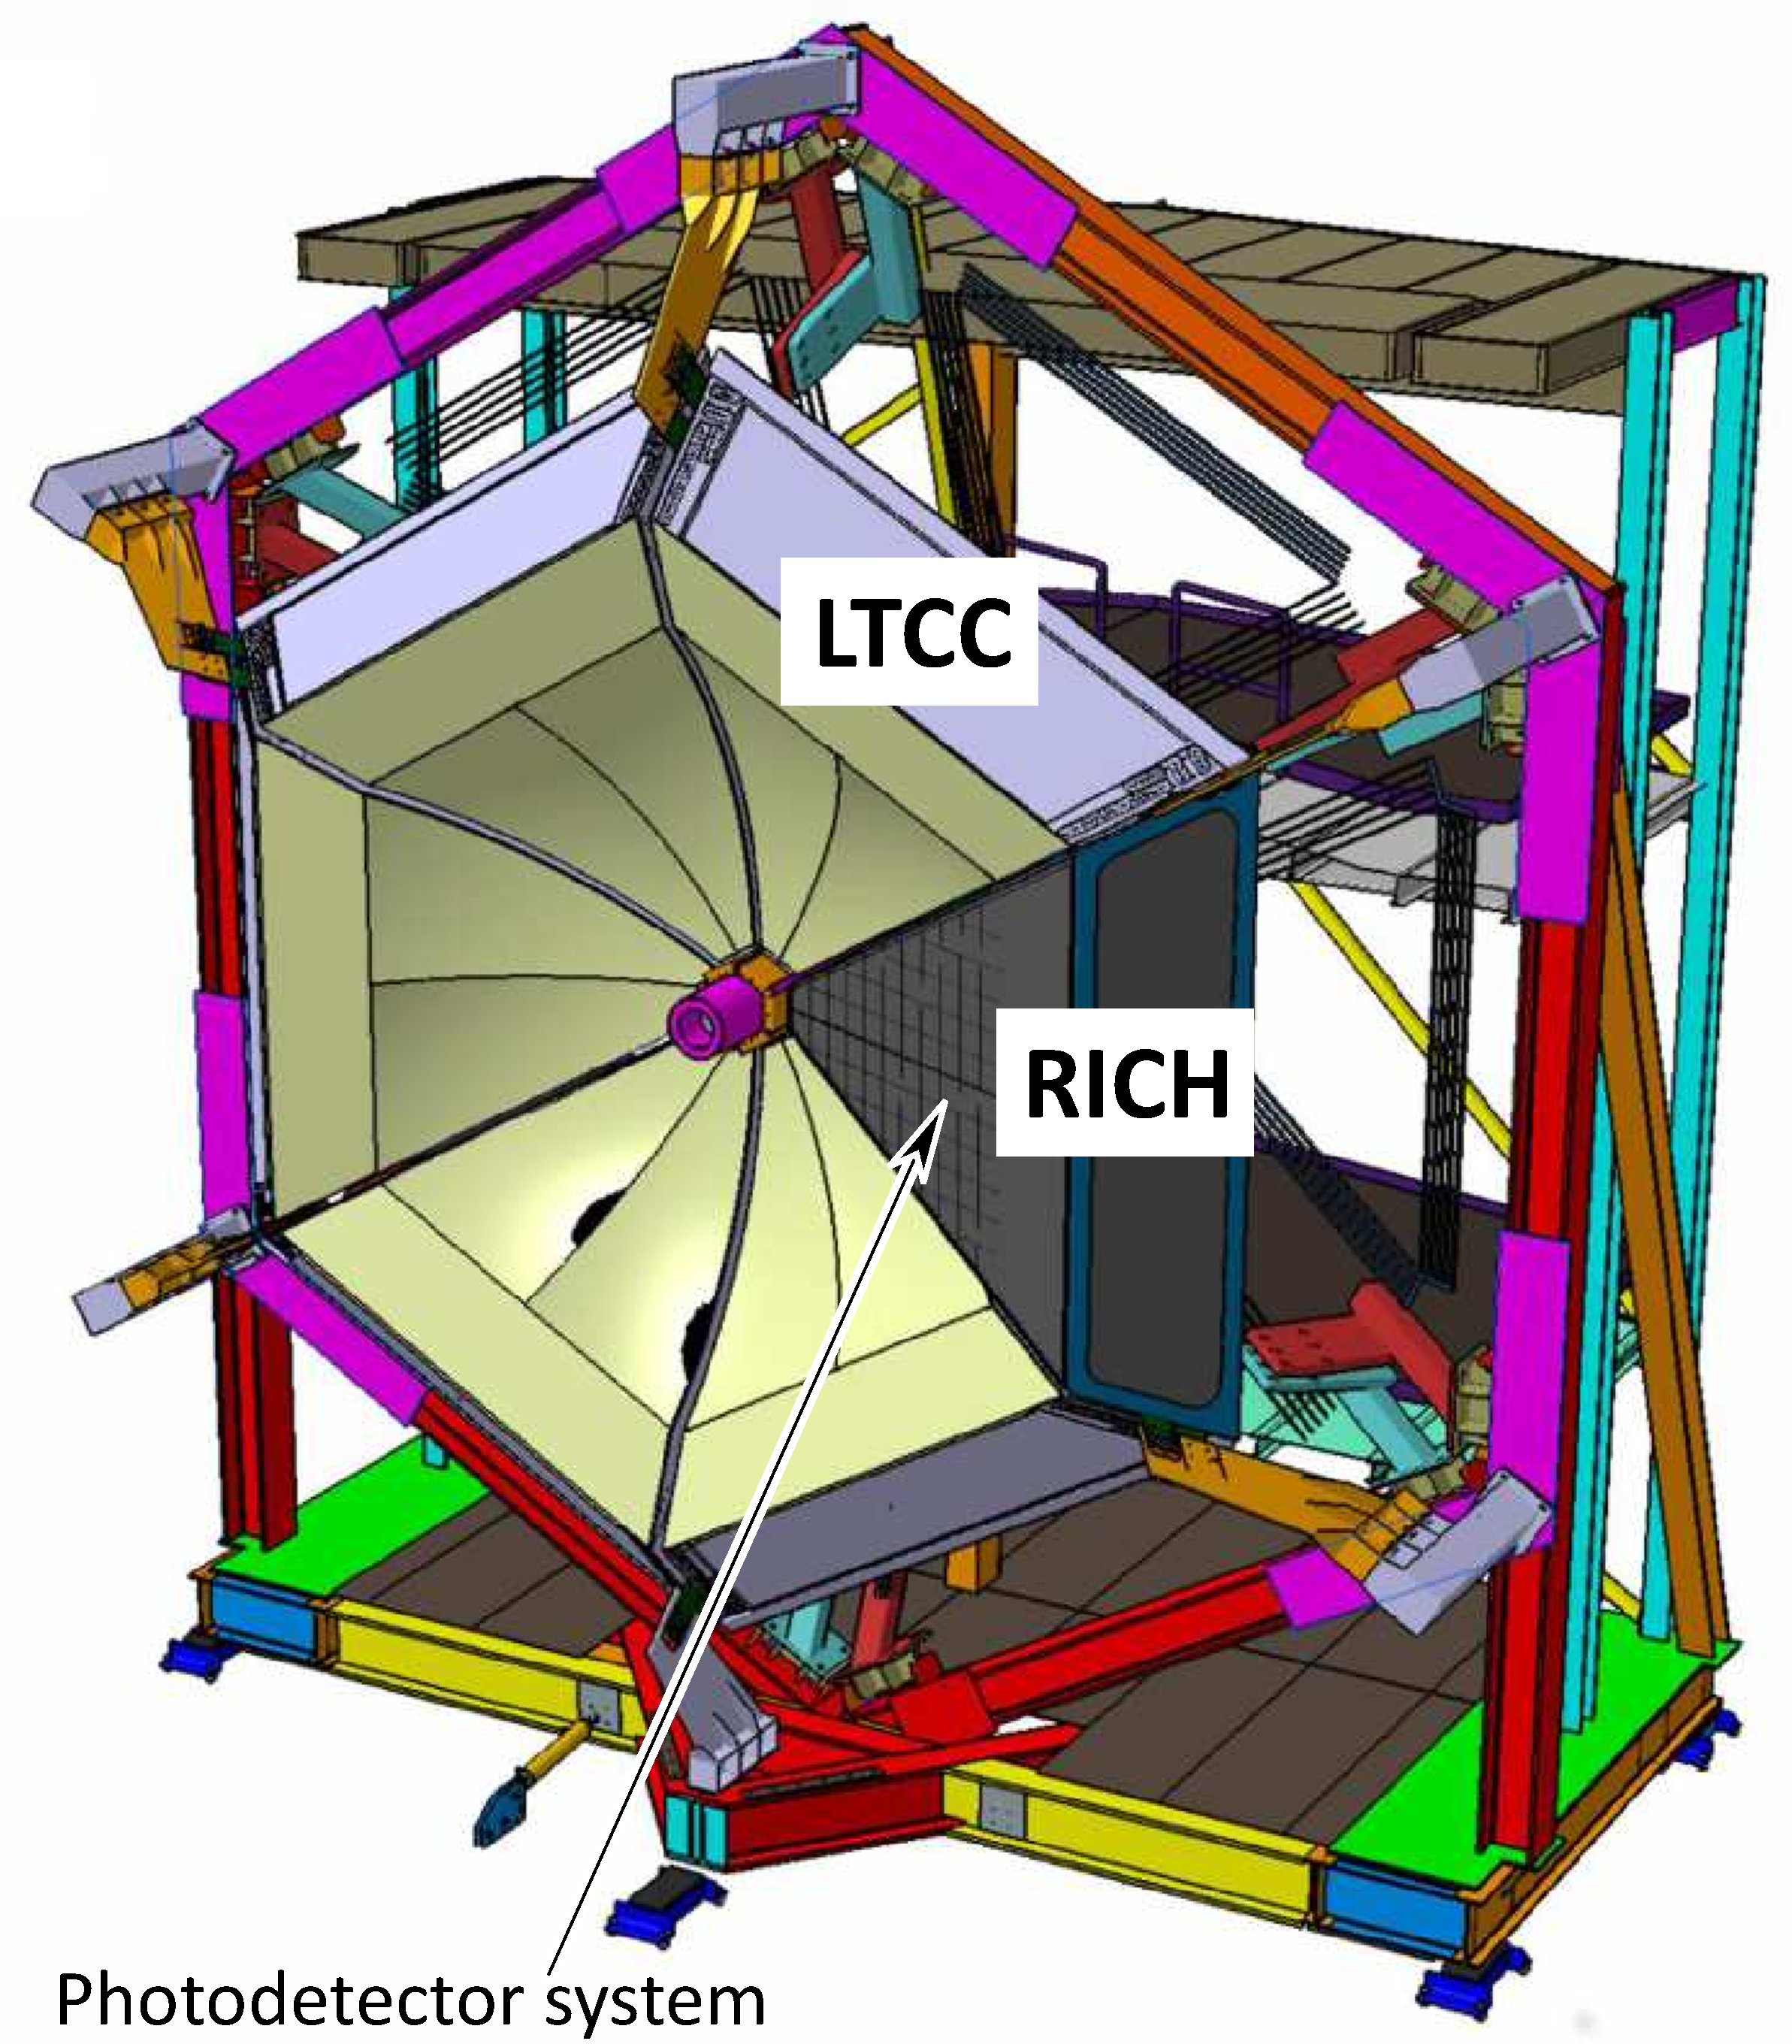
\includegraphics[width=0.95\linewidth]{figures/RICHdetector.pdf}
	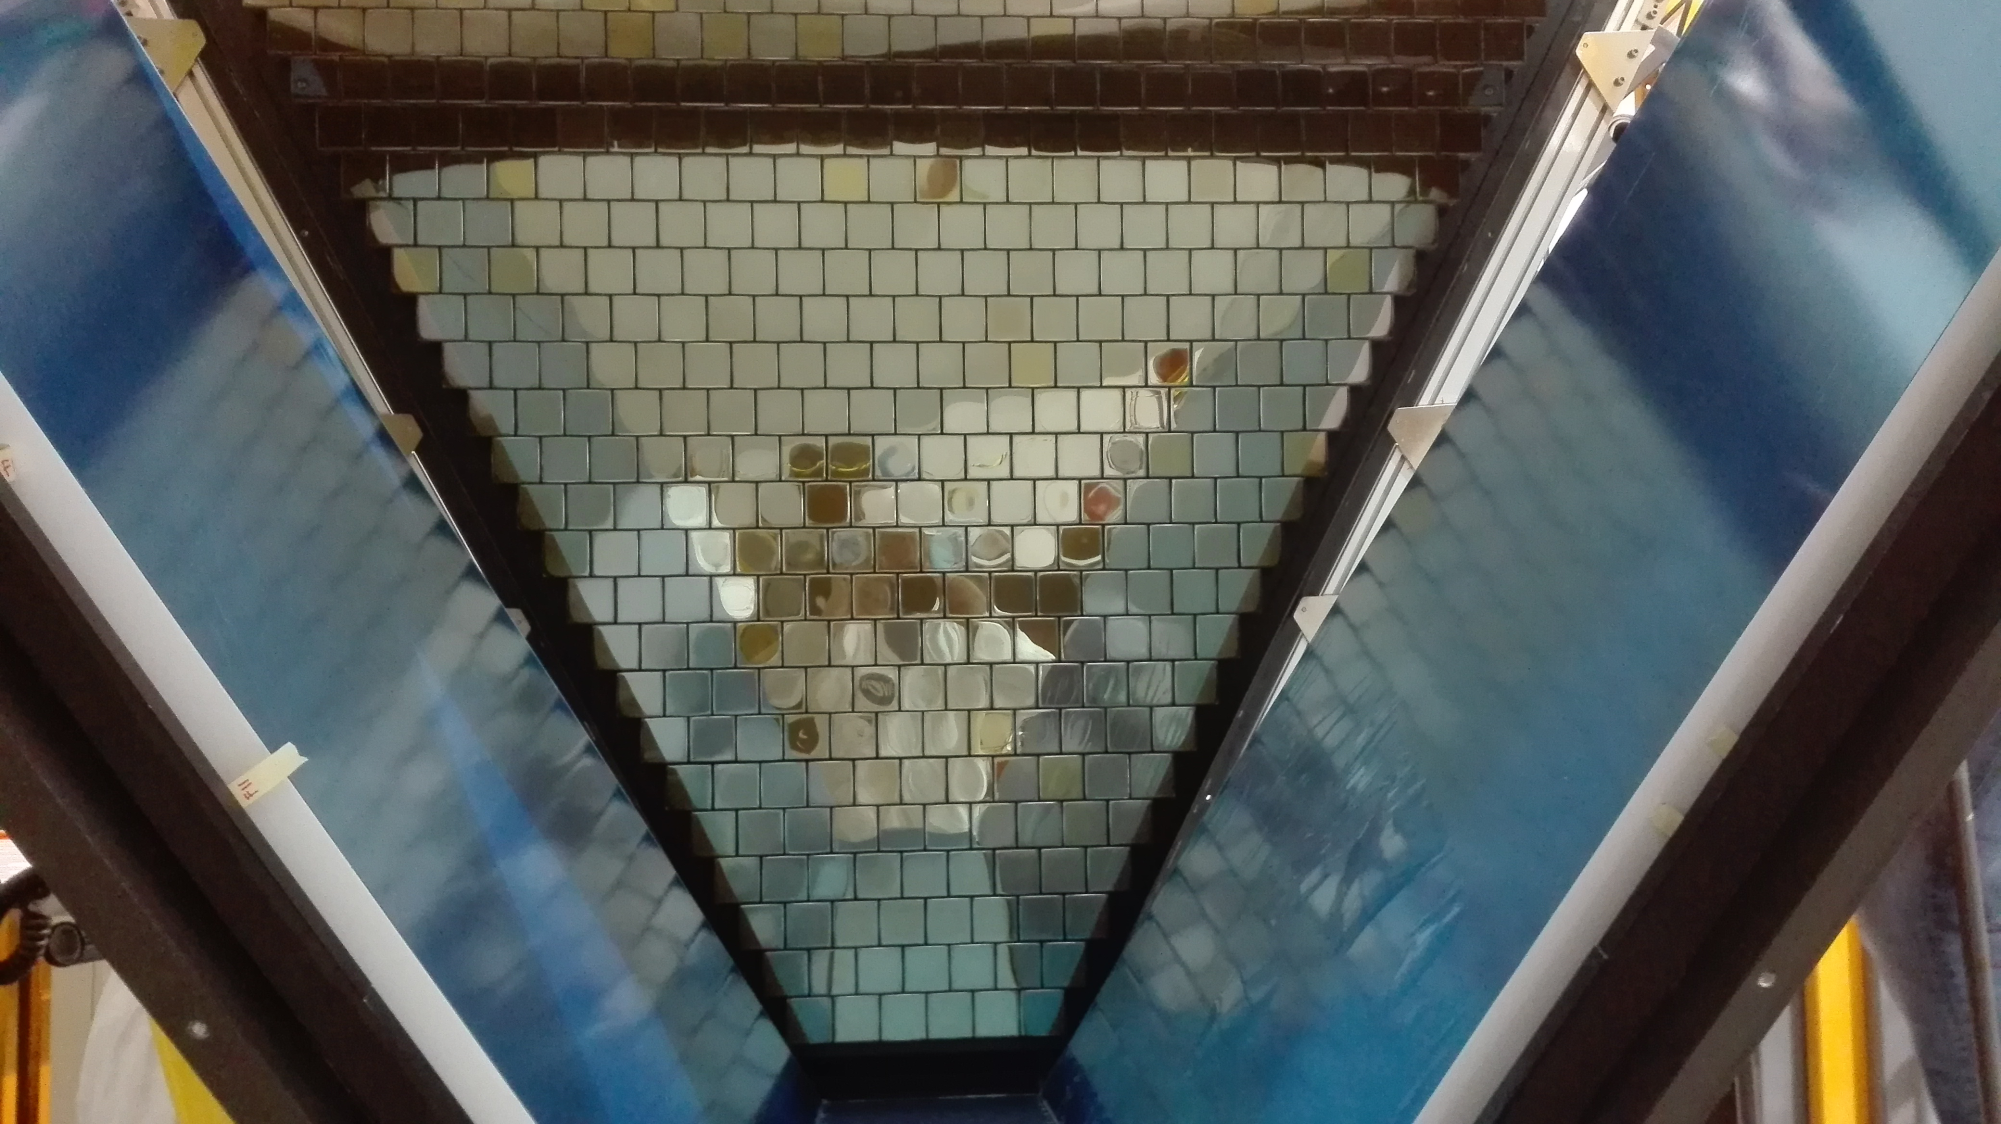
\includegraphics[width=0.95\linewidth]{figures/RICHpanel_front.png}
	\caption{Top: The part of the CLAS12 detector with the RICH covering one out of six sectors. Bottom: the photomatrix of multianode photomultipliers and the mirror system.}
	\label{fig:RICHdetector}
\end{figure}

The photomatrix  wall is a crucial component of the RICH detector (see Fig.~\ref{fig:RICHdetector}). It is relatively large (area about 1 m$^2$) and should be comprised of many photon detection devices such as photomultiplier tubes.
Due to the imaging aspect of the RICH they must provide a spatial resolution of less than 1 cm.
Since multiple photon detectors are tiled into large arrays, they should have large active area with minimal dead-space.
The photon detectors must also efficiently detect single photon level signals and should be sensitive to visible light due to the aerogel radiator material.
Multianode Photomultiplier Tubes from Hamamatsu are perfect candidates for the CLAS12 RICH detector, as they are flat-panel PMTs offering an adequate compromise between detector performance and cost.
Each MaPMT consists of an 8 by 8 array of pixels, each with dimension of 6~mm x 6~mm.
Furthermore, the device has a very high packing fraction of 89\% with a high quantum efficiency of 20-30\% in the visible light region.
The tubes also have excellent immunity to magnetic fields because all internal parts are housed in a metal package and the distance between dynode electrodes is very short.


Initially, the Hamamatsu H8500 MaPMT model \cite{H8500} was chosen as the best option because they provide high quantum efficiency for visible light and sufficient spatial resolution (6x6 mm$^2$) at a limited cost.
However, Hamamatsu has released the new H12700 MaPMT model  \cite{H12700} that shows enhanced single photoelectron (SPE) detection, reduced crosstalk between pixels, and is otherwise similar in spatial resolution and  cost to the H8500 MaPMTs.
The first RICH detector was installed in sector 4 of the CLAS12 detector in 2018.
There are 391 Hamamatsu MaPMTs  in the photodector matrix, 76 of them are H8500 and 315 H12700. 
The second RICH detector is almost identical to the first one and presently under construction scheduled to be installed soon.
%The initial characterization of these PMTs was done using a laser stand equipped with a crate of Flash ADC  boards \cite{FADC250} because the custom RICH front-end electronics \cite{RICH_FE} was not ready at that time.
The characterization of MaPMTs for both detectors was done using a laser stand equipped with custom front-end electronics boards which have much better parameters than the FADCs~\cite{FADC250} used for preliminary studies and installed in the most of the CLAS12 subsystems.
This highly integrated front-end (FE) electronics with modular design~\cite{RICH_FE} was developed for a large array of Hamamatsu H8500 and H12700 MaPMTs to minimize the impact of the electronics material on the CLAS12 subsystems downstream of the RICH detector.
The architecture of the readout electronics consists of front-end cards with dedicated Application Specific Integrated Circuits (ASICs), configured, controlled, and read out by Field Programmable Gate Arrays (FPGAs) \cite{RICH_FE}.
The ASIC board is based on the MAROC3  integrated circuit \cite{MAROC} whose excellent single photon capabilities both in analog and binary mode have been confirmed.
%The final design has consists of stacked PCB layers behind each MaPMT sensor (see~Fig.~\ref{fig:feboards}).
%The first layer houses the ASIC front end and ancillary components (e.g. external amplifier) and it is directly connected to the anodes array.
%A second PCB will host the FPGA in charge of configuring, managing and acquiring one or more ASICs and the low voltage and HV bias distribution.
%The use of the JLab SSP as controller and collector of the front-end data provides a strong synergy with the current JLab upgrade activity.
%Data are transmitted on high speed serial (optical) lines minimizing the wiring and therefore the material budget.
%With that sandwich architecture the total photon detection surface will be covered by a fixed number of basic units or tiles made up by two or three sensor each.
%The total spacing for electronics will not exceed 20 cm in depth (including MaPMT and mechanical support).
The three-tile electronics module with and without the three H12700 MaPMTs installed is shown in~Fig.~\ref{fig:feboards}.
The performance of the MAROC chips was tested and was found suitable for the RICH requirements:
\begin{itemize}
	\item 100\% efficiency at 1/3 of the single photoelectron signal (50~fC)
	\item time resolution of 1~ns
	\item short deadtime to sustain a trigger rate of 30~kHz
	\item latency of 8~$\mu$s
\end{itemize}
We made detailed characterization of around 400 H12700 MaPMTs, as well as several H8500 to make a comparison of the two models. These data turned out to be useful for evaluating the performance of the first CLAS12 RICH detector where both MaPMT models are used. The single photoelectron spectra were measured for each pixel at different high voltages and light intensities of the laser test setup. Using the dedicated front-end electronics, standard for the RICH detectors, the setup allowed us to characterize each pixel’s properties such as gain, quantum efficiency, signal crosstalk between neighboring pixels, and determine the signal threshold values to optimize their efficiency to detect Cherenkov photons. These parameters were determined for each pixel in the set of 400 MaPMTs, giving us the opportunity to select the best MaPMTs and determine the working parameters of the front-end electronics in the real experiment. The results of this study are presented in this paper. 
%These data turned out to be useful for evaluating the first RICH performance  where we are using both MaPMT models. The single photoelectron spectra were measured for each pixel at different high voltages and light intensities of the laser test setup. Using the standard for RICH dedicated front-end electronics the setup allowed us to characterize each pixel’s properties such as gain, quantum efficiency, signal crosstalk between neighboring pixels, and determine the signal threshold values to optimize their efficiency to detect Cherenkov photons. These parameters were determined for each pixel out of 400 MaPMTs what gives us the possibility to select the best MaPMTs and determine the working parameters of the front-end electronic in the real experiment. The results of this study are presented in this paper. 


The remaining structure of this paper is laid out as follows. 
\begin{itemize}
	\item Section 2 presents the design of the laser test stand for the MaPMT automated characterization, allowing illumination of every pixel by the precisely calibrated low light pulses in the controlled stable environment, and collecting the response data. 
	\item Section 3 describes the procedures for the absolute calibration of the readout electronics converting the output signal amplitudes to linear charge scale in pC for every pixel. 
	\item Section 4 illustrates the techniques for the pixel-to-pixel crosstalk measurements, and possible algorithms for the separation of the crosstalk from real signals. 
	\item Section 5 describes the technique of absolute calibration of the light source, as a prerequisite for the measurement of quantum efficiency in every pixel. 
	\item Section 6 describes the computational model used in the data analysis to extract such critical parameters for each anode, as its quantum efficiency, gain, the shape of the single photoelectron amplitude response function, and contribution of the crosstalk signals from the neighboring pixels, and introducing the novel technique of characterizing the crosstalk contributions in the model. 
	\item Section 7 illustrates the self-consistency of the algorithm for the parameters' extraction using the measurements at different light intensities and different high voltages applied. 
	\item Section 8 presents the results of the full characterization and study of all 399 MaPMTs, showing the spread of the extracted parameters and evaluating the systematic errors from the independent redundant measurements. The results make possible the evaluation of average and individual pixel characteristics of the full MaPMT array for the purposes of selection and arrangement of the MaPMTs in the RICH detector, and for use in the experimental data analysis.
\end{itemize}

\begin{figure}[htb]
  \centering
  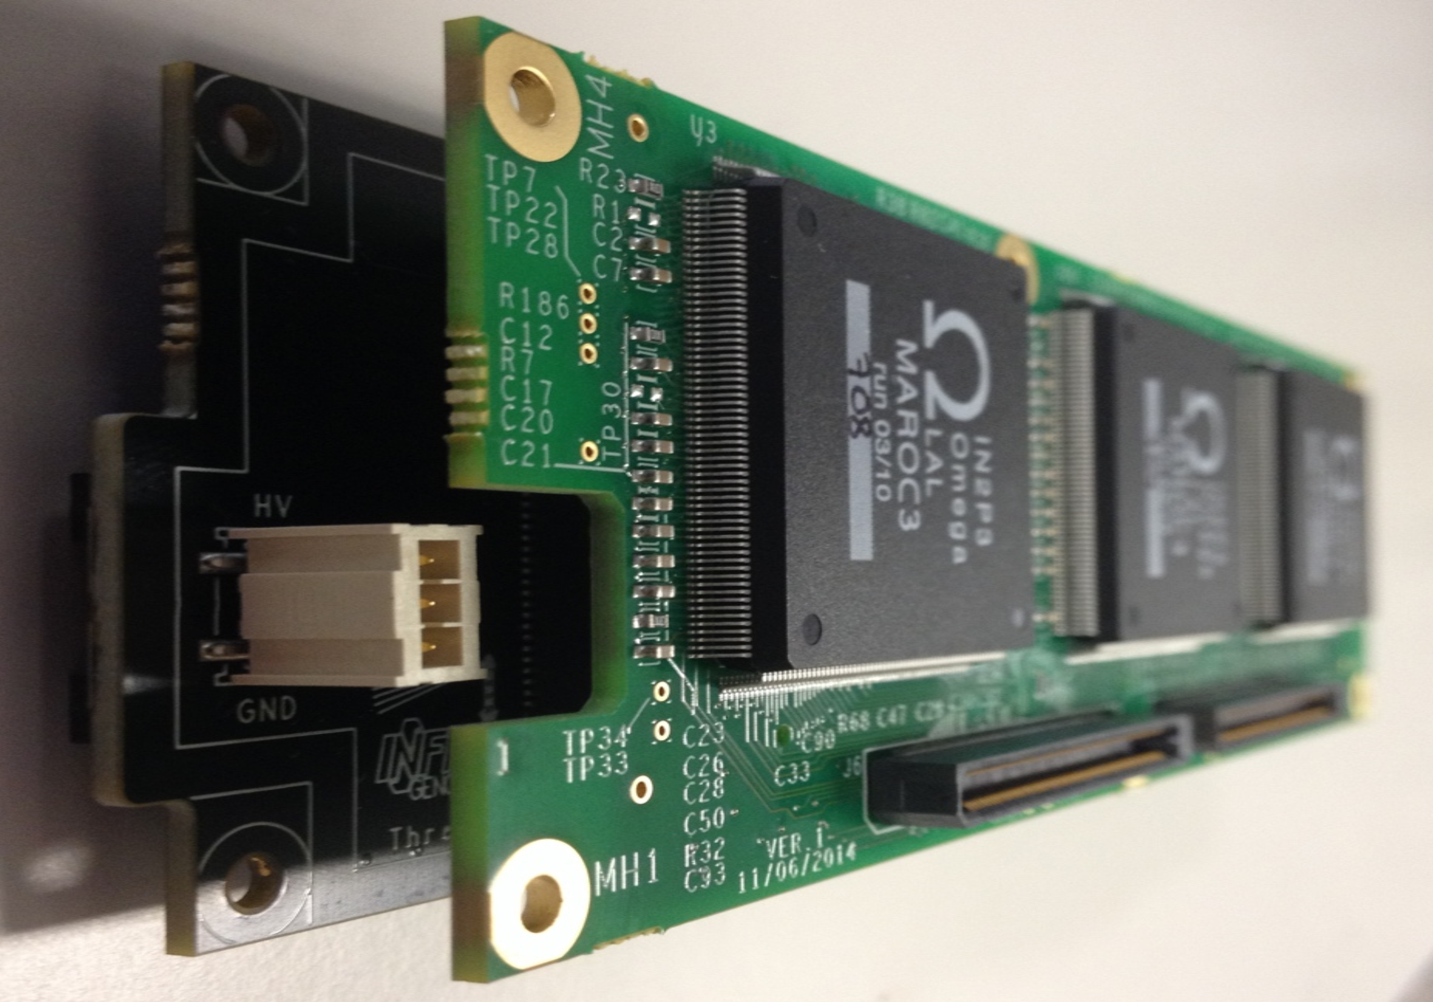
\includegraphics[width=0.8\linewidth]{figures/fe1.pdf}
  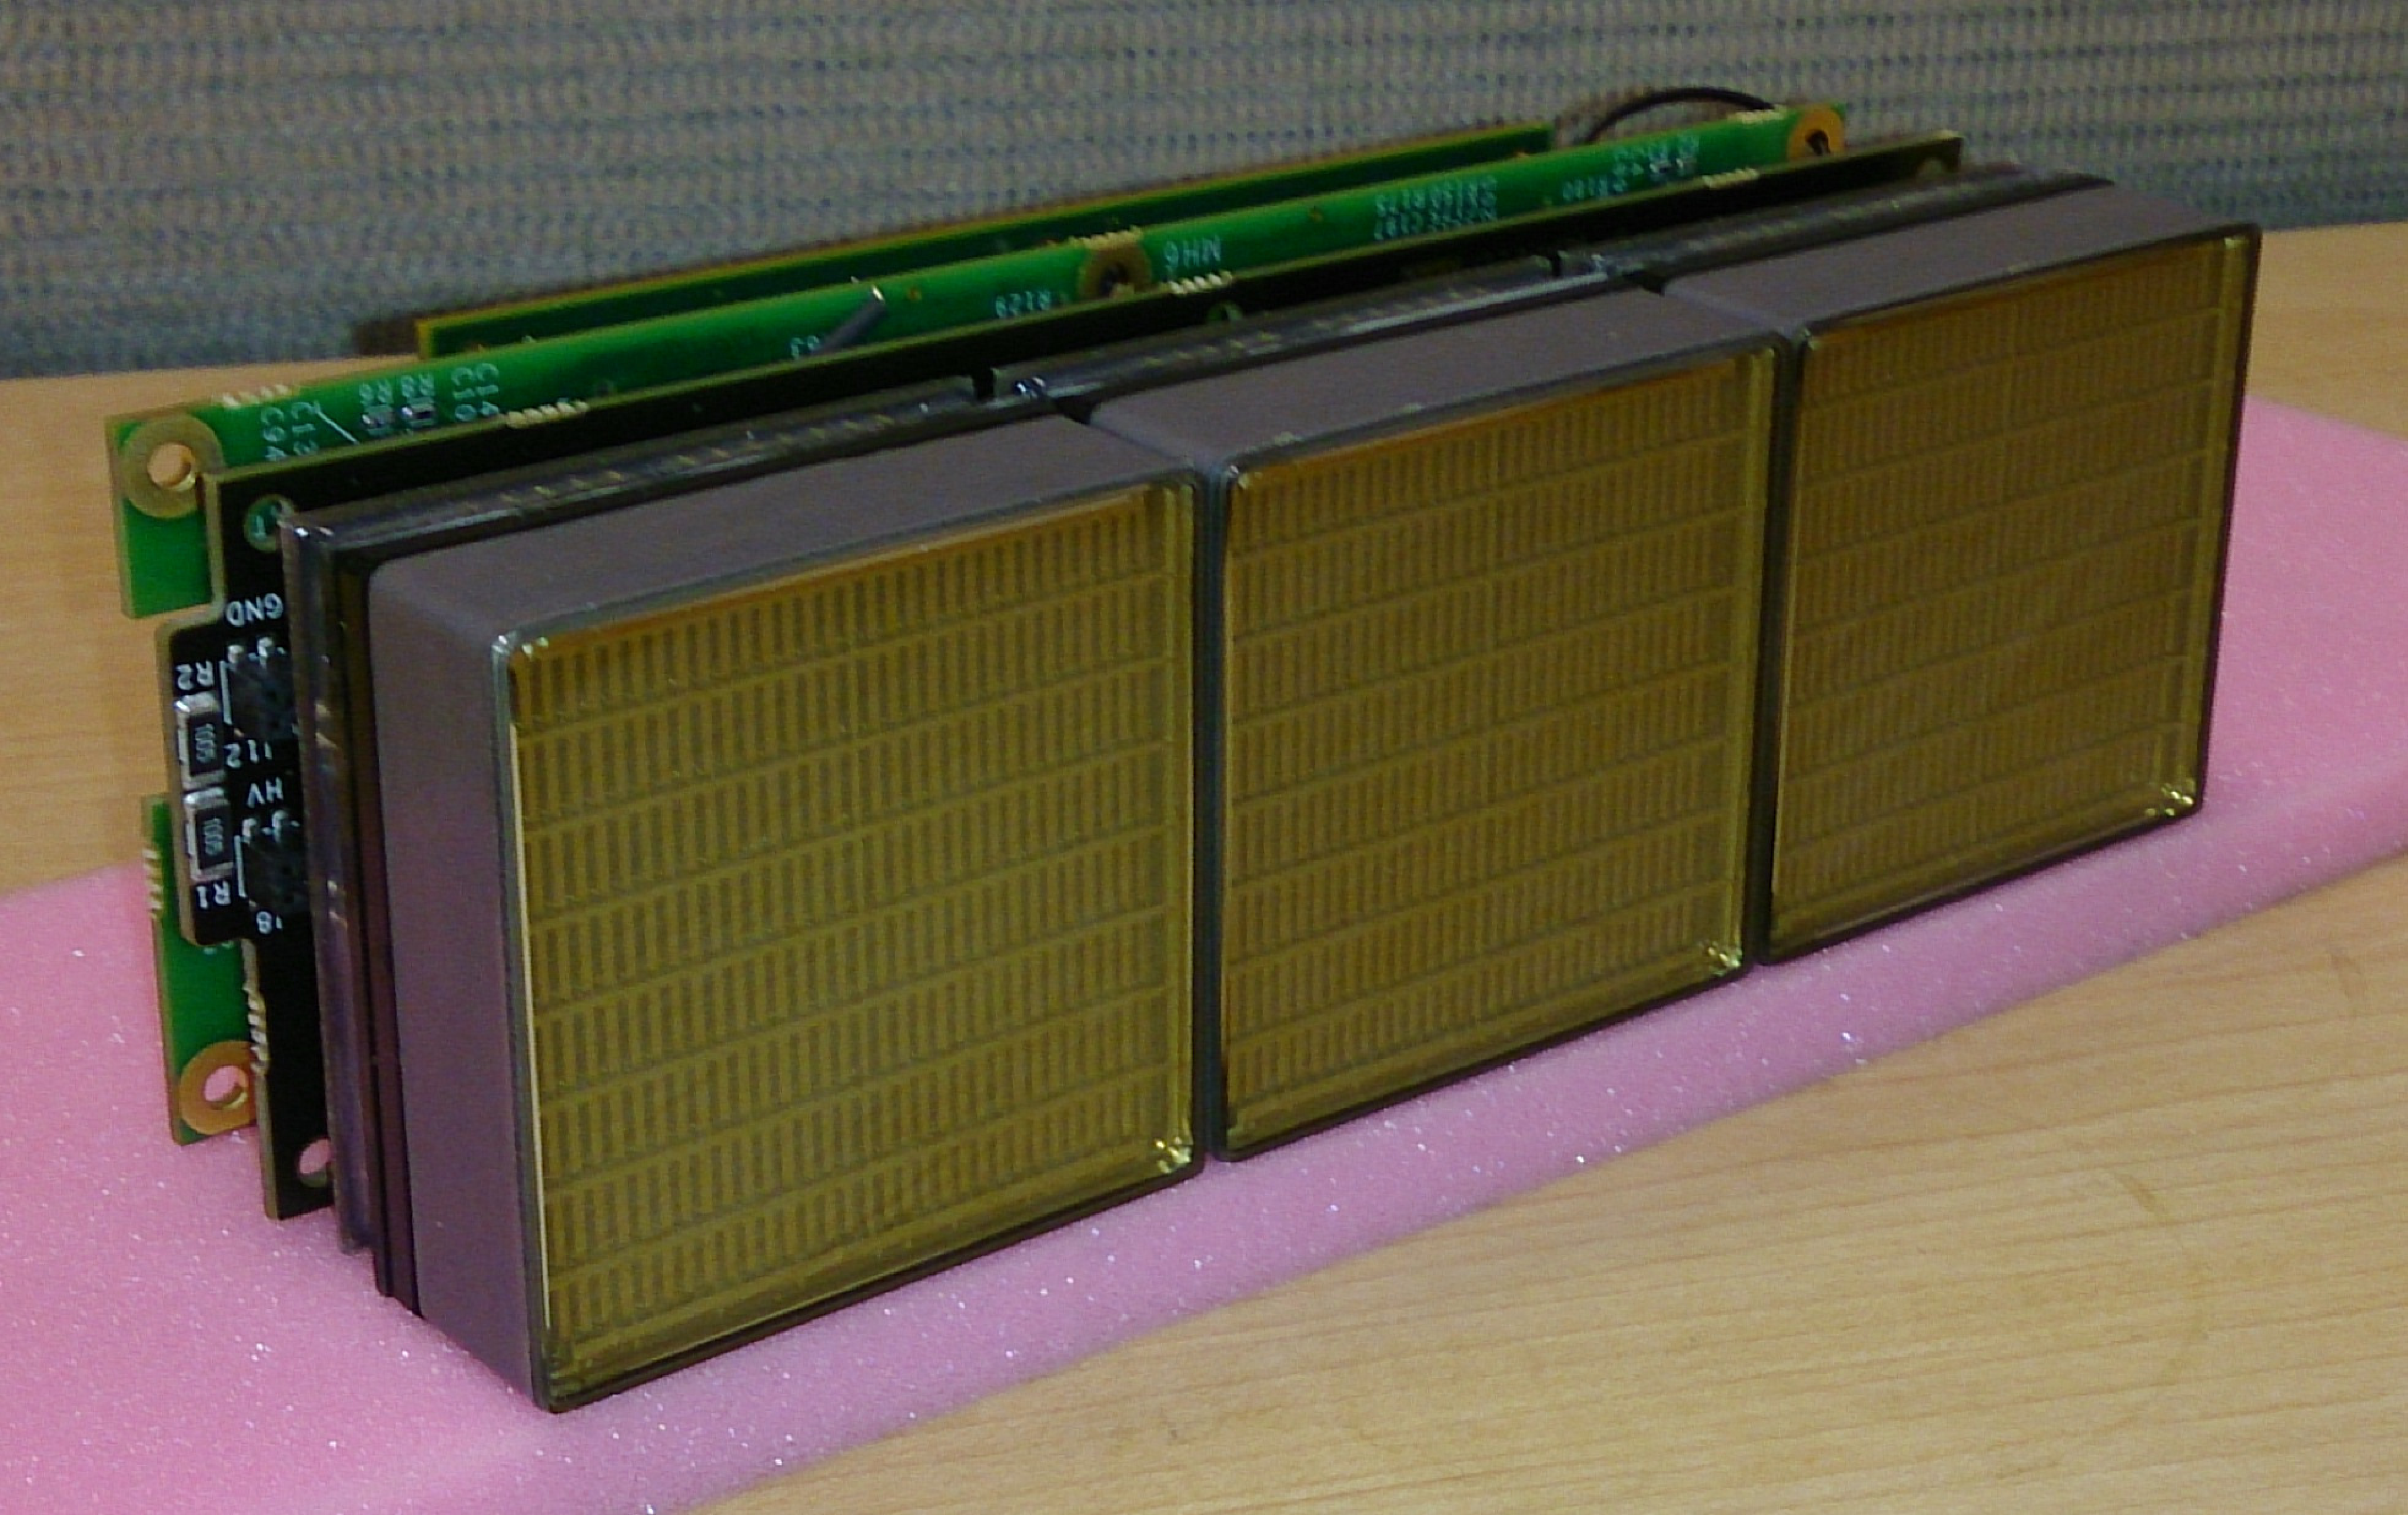
\includegraphics[width=0.8\linewidth]{figures/frontendPMT.pdf}
  \caption{Front-end electronics readout board and mounted MaPMTs.}
  \label{fig:feboards}
\end{figure}






	  % vpk

\section{Laser stand for the MAPMT characterization}
The large number of the channels in the RICH detector  poses challenging problem for the MAPMT testing and calibration.
RICH consists of 391 MAPMTs resulting in total number of channels equal to 25024. So in order to test them efficiently within a reasonable timeframe the fully automated test stand was build to evaluate 6 MAPMTs at once, as shown on Fig.~\ref{fig:MAPMTtest}.

\begin{figure}[hbt]
	\centering
	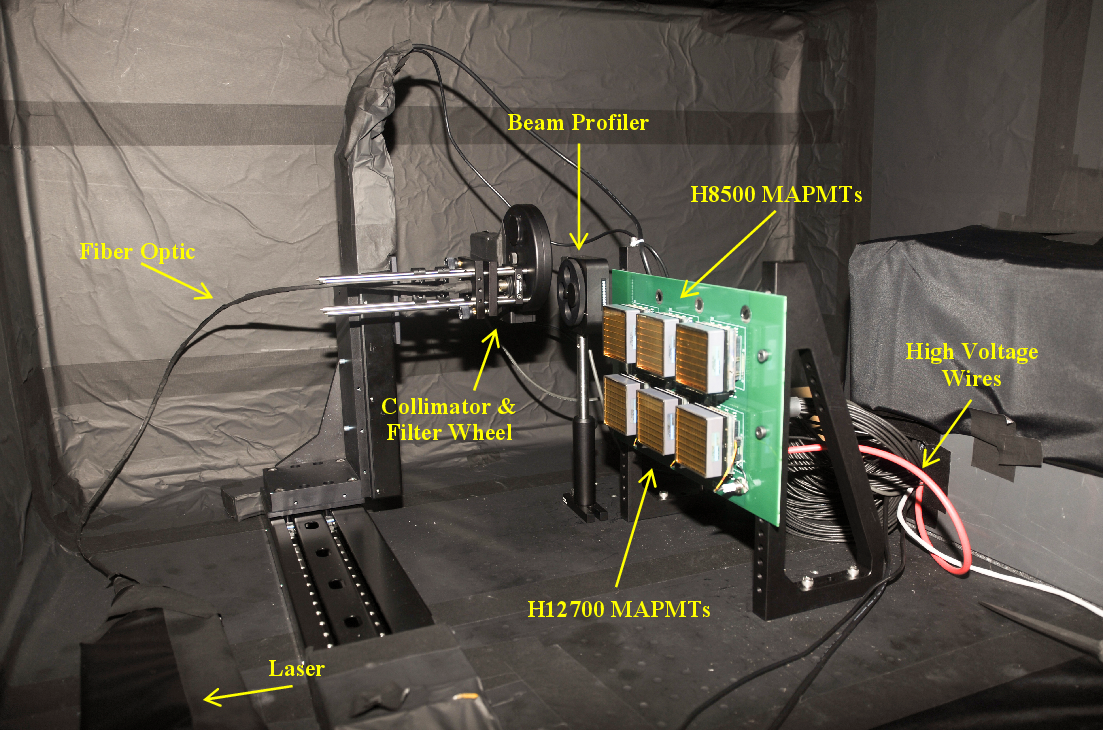
\includegraphics[width=0.9\linewidth]{figures/blackbox.png}
	\caption{Inner view of the laser stand.}
	\label{fig:MAPMTtest}
\end{figure}

The test stand consists of picosecond diode  laser PiL047X with 470 nm wavelength, 2 long travel motorized stands to drive laser fiber in two dimensional space for individual pixel illumination, the motorized wheel with neutral density filter system, 2 adapter boards for MAPMT with JLab designed front-end electronics boards \cite{}{Contalbrigo:2020}.
The laser light is directed through the fiber and attenuated to the single photon level using the neutral density filters to mimic the conditions of the RICH detector.
The motors were remotely controlled to move the focused laser beam across (see Fig.~\ref{fig:beamopt1}) the entire surface of the MAPMT entrance window and illuminate one by one of all its 64 pixels individually.
Another option is to illuminate the whole surface of MAPMT photocathode at once using the Engineered Diffuser to produce square pattern with non-Gaussian intensity distribution (see Fig.~\ref{fig:beamopt2}). 

All laser stand equipment is sitting in the black box with non-reflective black material on the optical table. The laser interlock safety box automatically switch off laser, as well as front-end low voltage  electronics and MAPMT high voltage to prevent the possible photomultiplier damage or laser light human illumination in case if somebody will try to open the front door of the black box during the measurements.

\begin{figure}[bt]
	\centering
	\begin{subfigure}[b]{0.628\linewidth}
		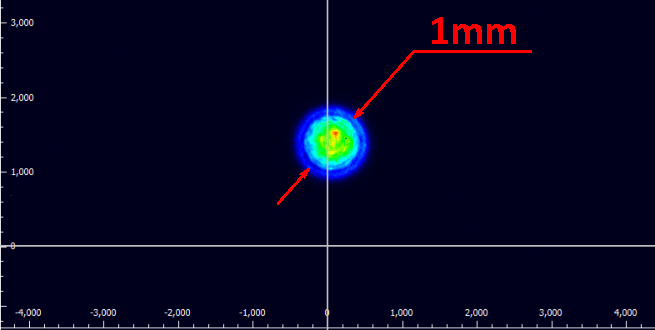
\includegraphics[width=\linewidth]{figures/beamspot.pdf}
		\caption{Focused laser beam with the dimension much less than the  MAPMT pixel size.}
		\label{fig:beamopt1}
	\end{subfigure}
	\begin{subfigure}[b]{0.354\linewidth}
		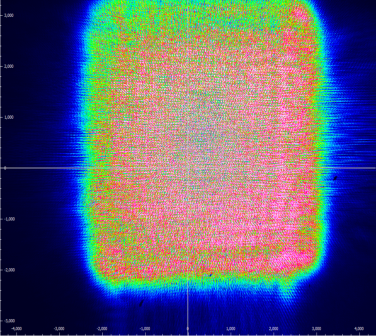
\includegraphics[width=\linewidth]{figures/beamsquare.pdf}
		\caption{Square pattern illuminated all MAPMT surface.}
		\label{fig:beamopt2}
	\end{subfigure}
	\caption{The laser light output options.}
\end{figure}

This configuration brings routine workload to minimum allowing the evaluation of 6 MAPMTs (equivalent to 328 conventional PMTs!) at 4 different high voltages and 6 different light intensities within 6 hours with less than 15 minutes of human intervention needed to load the MAPMTs to the front-end boards.

\begin{figure}[b]
	\centering
	\begin{subfigure}{0.3\linewidth}
		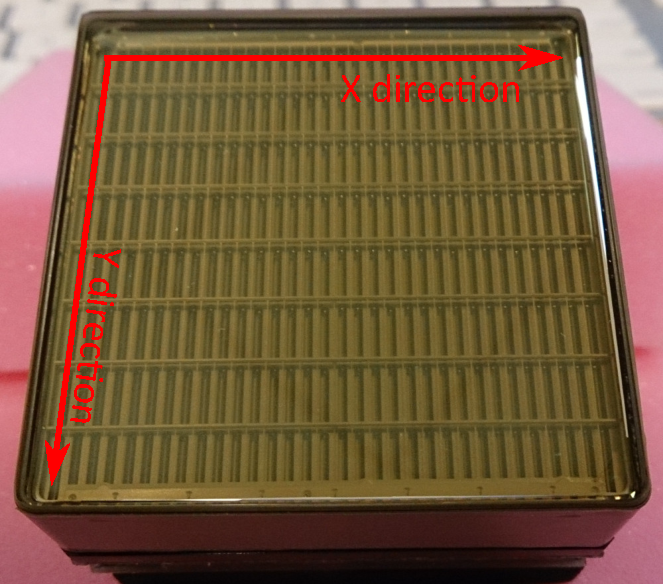
\includegraphics[width=\linewidth]{figures/surfaceuniform1.pdf}
		\caption{MAPMT with visible internal structure of metal channel dynodes and focusing mesh.}
		\label{fig:surfaceuniform1}
	\end{subfigure}
	\quad
	\begin{subfigure}{0.3\linewidth}
		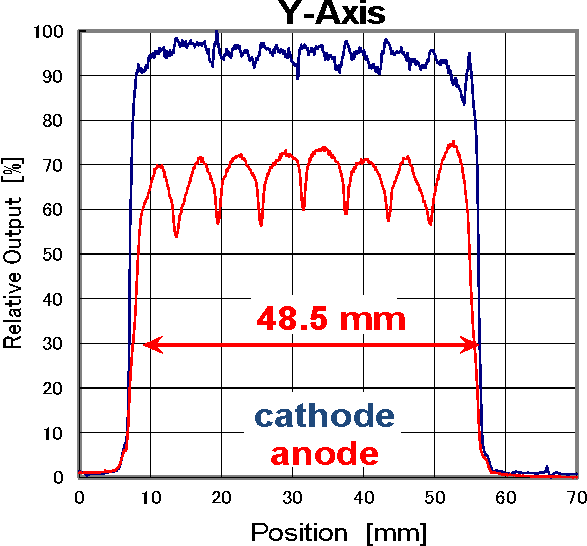
\includegraphics[width=\linewidth]{figures/surfaceuniform3.pdf}
		\caption{The response along the X axis; the signal drops in the deadspace between the pixels.}
		\label{fig:surfaceuniform2}
	\end{subfigure}
	\quad
	\begin{subfigure}{0.3\linewidth}
		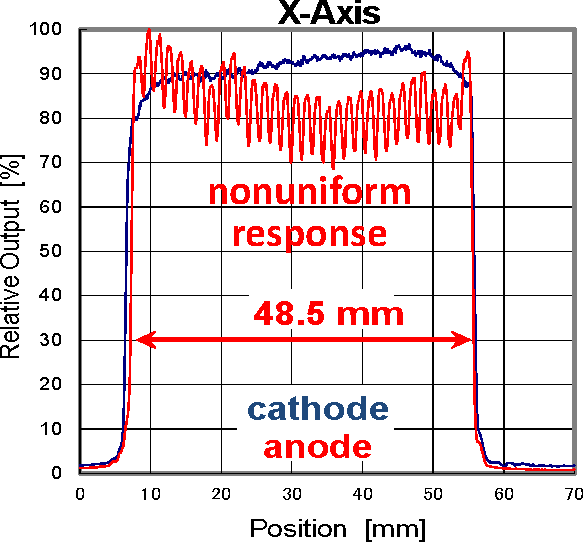
\includegraphics[width=\linewidth]{figures/surfaceuniform2.pdf}
		\caption{The response along the Y axis: multiple segmentations within the pixels.}
		\label{fig:surfaceuniform3}
	\end{subfigure}
	\caption{The response uniformity of MAPMT.}
	\label{fig:surfaceuniform}
\end{figure}


Before starting the systematic study of the MAPMT responses, a finer two dimensional scan of several pixels was performed in order to verify the uniformity of the response across pixel's surfaces, as shown on Fig.~\ref{fig:surfaceuniform}.
The horizontal and vertical axes denote laser beam position during the scan.
Along the both directions there are obvious drops in efficiency when the laser strikes the space between the pixels.
The drops are relatively narrow so the dead-space is very small as expected from the Hamamatsu specifications.
Additionally, a vertical efficiency variation is visible across the pixel in horizontal scan.
These inhomogeneities are correlated with the vertical walls separating dynode chains, owing to the constructional features of the MAPMT. The discontinuity in dynode structure is visible  on Fig.~\ref{fig:surfaceuniform1}.
The separate response maps for photocathode shows relatively uniform signal without efficiency drops, confirming that the variation arises from the dynode system.
  	  % Andrey
%\clearpage
%\section{Front-end electronics$^{}$}

The highly integrated front-end (FE) electronics with modular design was developed for a large array of Hamamatsu H8500 and H12700 MAPMTs to minimize the impact of the electronics material on CLAS12 subsystems downstream RICH detector.
An architecture of the readout electronics consists of front-end cards with dedicated Application Specific Integrated Circuit (ASIC) configured, controlled and readout by programmable devices such as Field Programmable Gate Array (FPGA) \cite{RICH_FE}.
The ASIC board is based on the MAROC3  integrated circuit \cite{MAROC} whose excellent single photon capabilities both in analog and binary mode have been confirmed.
%The final design has consists of stacked PCB layers behind each MAPMT sensor (see~Fig.~\ref{fig:feboards}).
%The first layer houses the ASIC front end and ancillary components (e.g. external amplifier) and it is directly connected to the anodes array.
%A second PCB will host the FPGA in charge of configuring, managing and acquiring one or more ASICs and the low voltage and HV bias distribution.
%The use of the JLab SSP as controller and collector of the front-end data provides a strong synergy with the current JLab upgrade activity.
%Data are transmitted on high speed serial (optical) lines minimizing the wiring and therefore the material budget.
%With that sandwich architecture the total photon detection surface will be covered by a fixed number of basic units or tiles made up by two or three sensor each.
%The total spacing for electronics will not exceed 20 cm in depth (including MAPMT and mechanical support).
The three-tiles electronics module with and without 3 H12700 MAPMTs installed is shown on~Fig.~\ref{fig:feboards}.
The performance of MAROC chips was tested and was found suitable for RICH requirements:
\begin{itemize}
	\item 100\% efficiency at 1/3 of single photoelectron signal (50~fC)
	\item time resolution of 1~ns
	\item short deadtime to sustain the trigger rate of 20~kHz
	\item latency of 8~$\mu s$
\end{itemize}

\begin{figure}[htb]
  \centering
  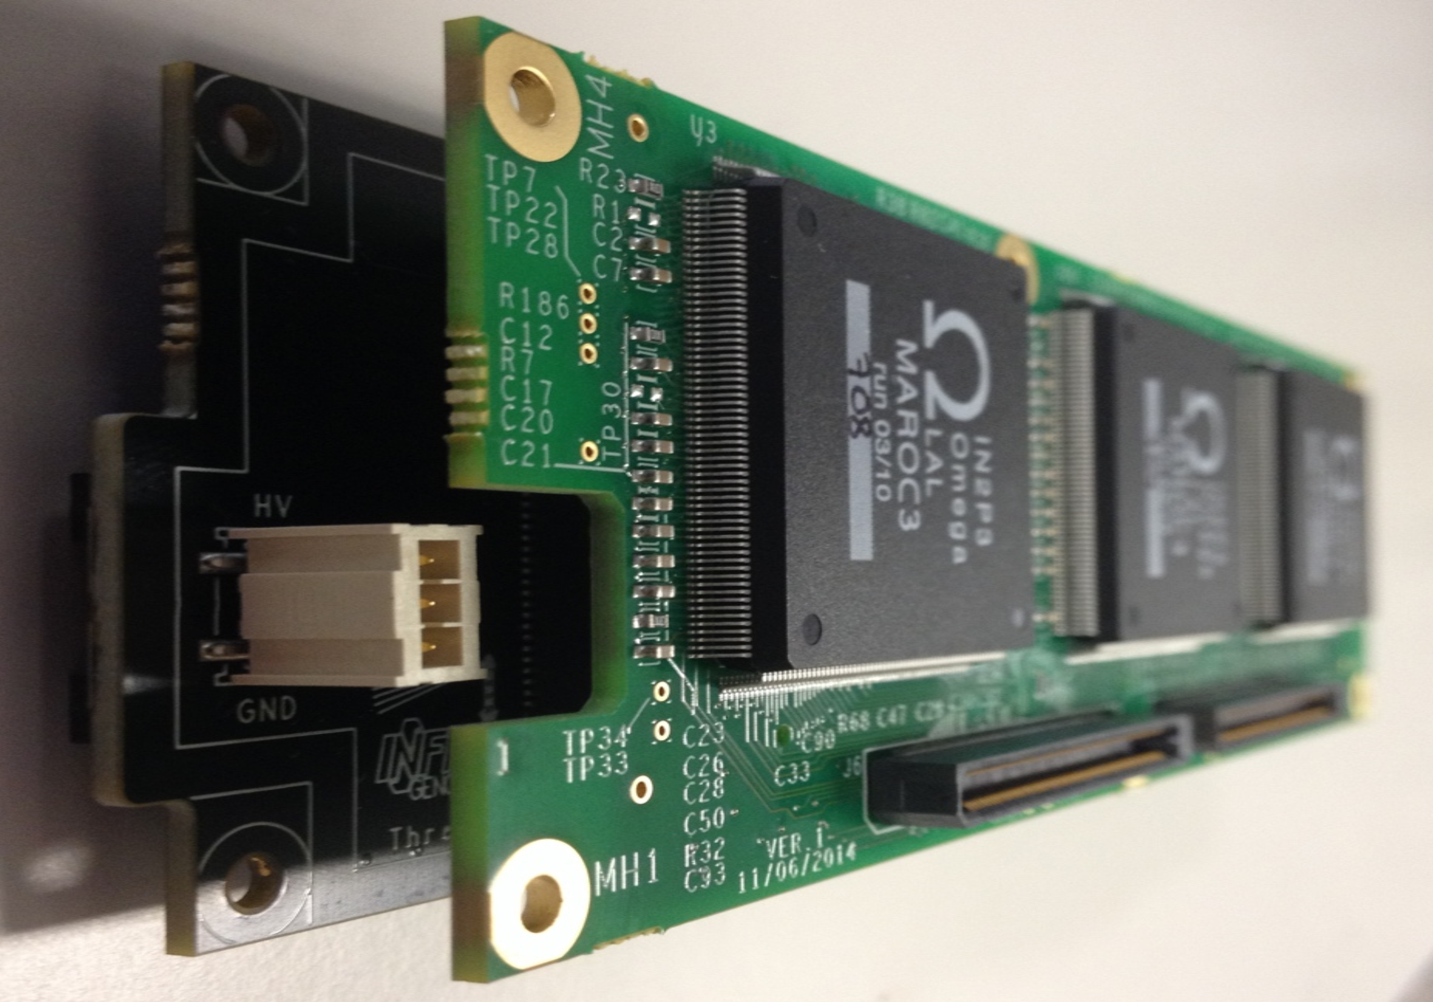
\includegraphics[width=0.8\linewidth]{figures/fe1.pdf}
  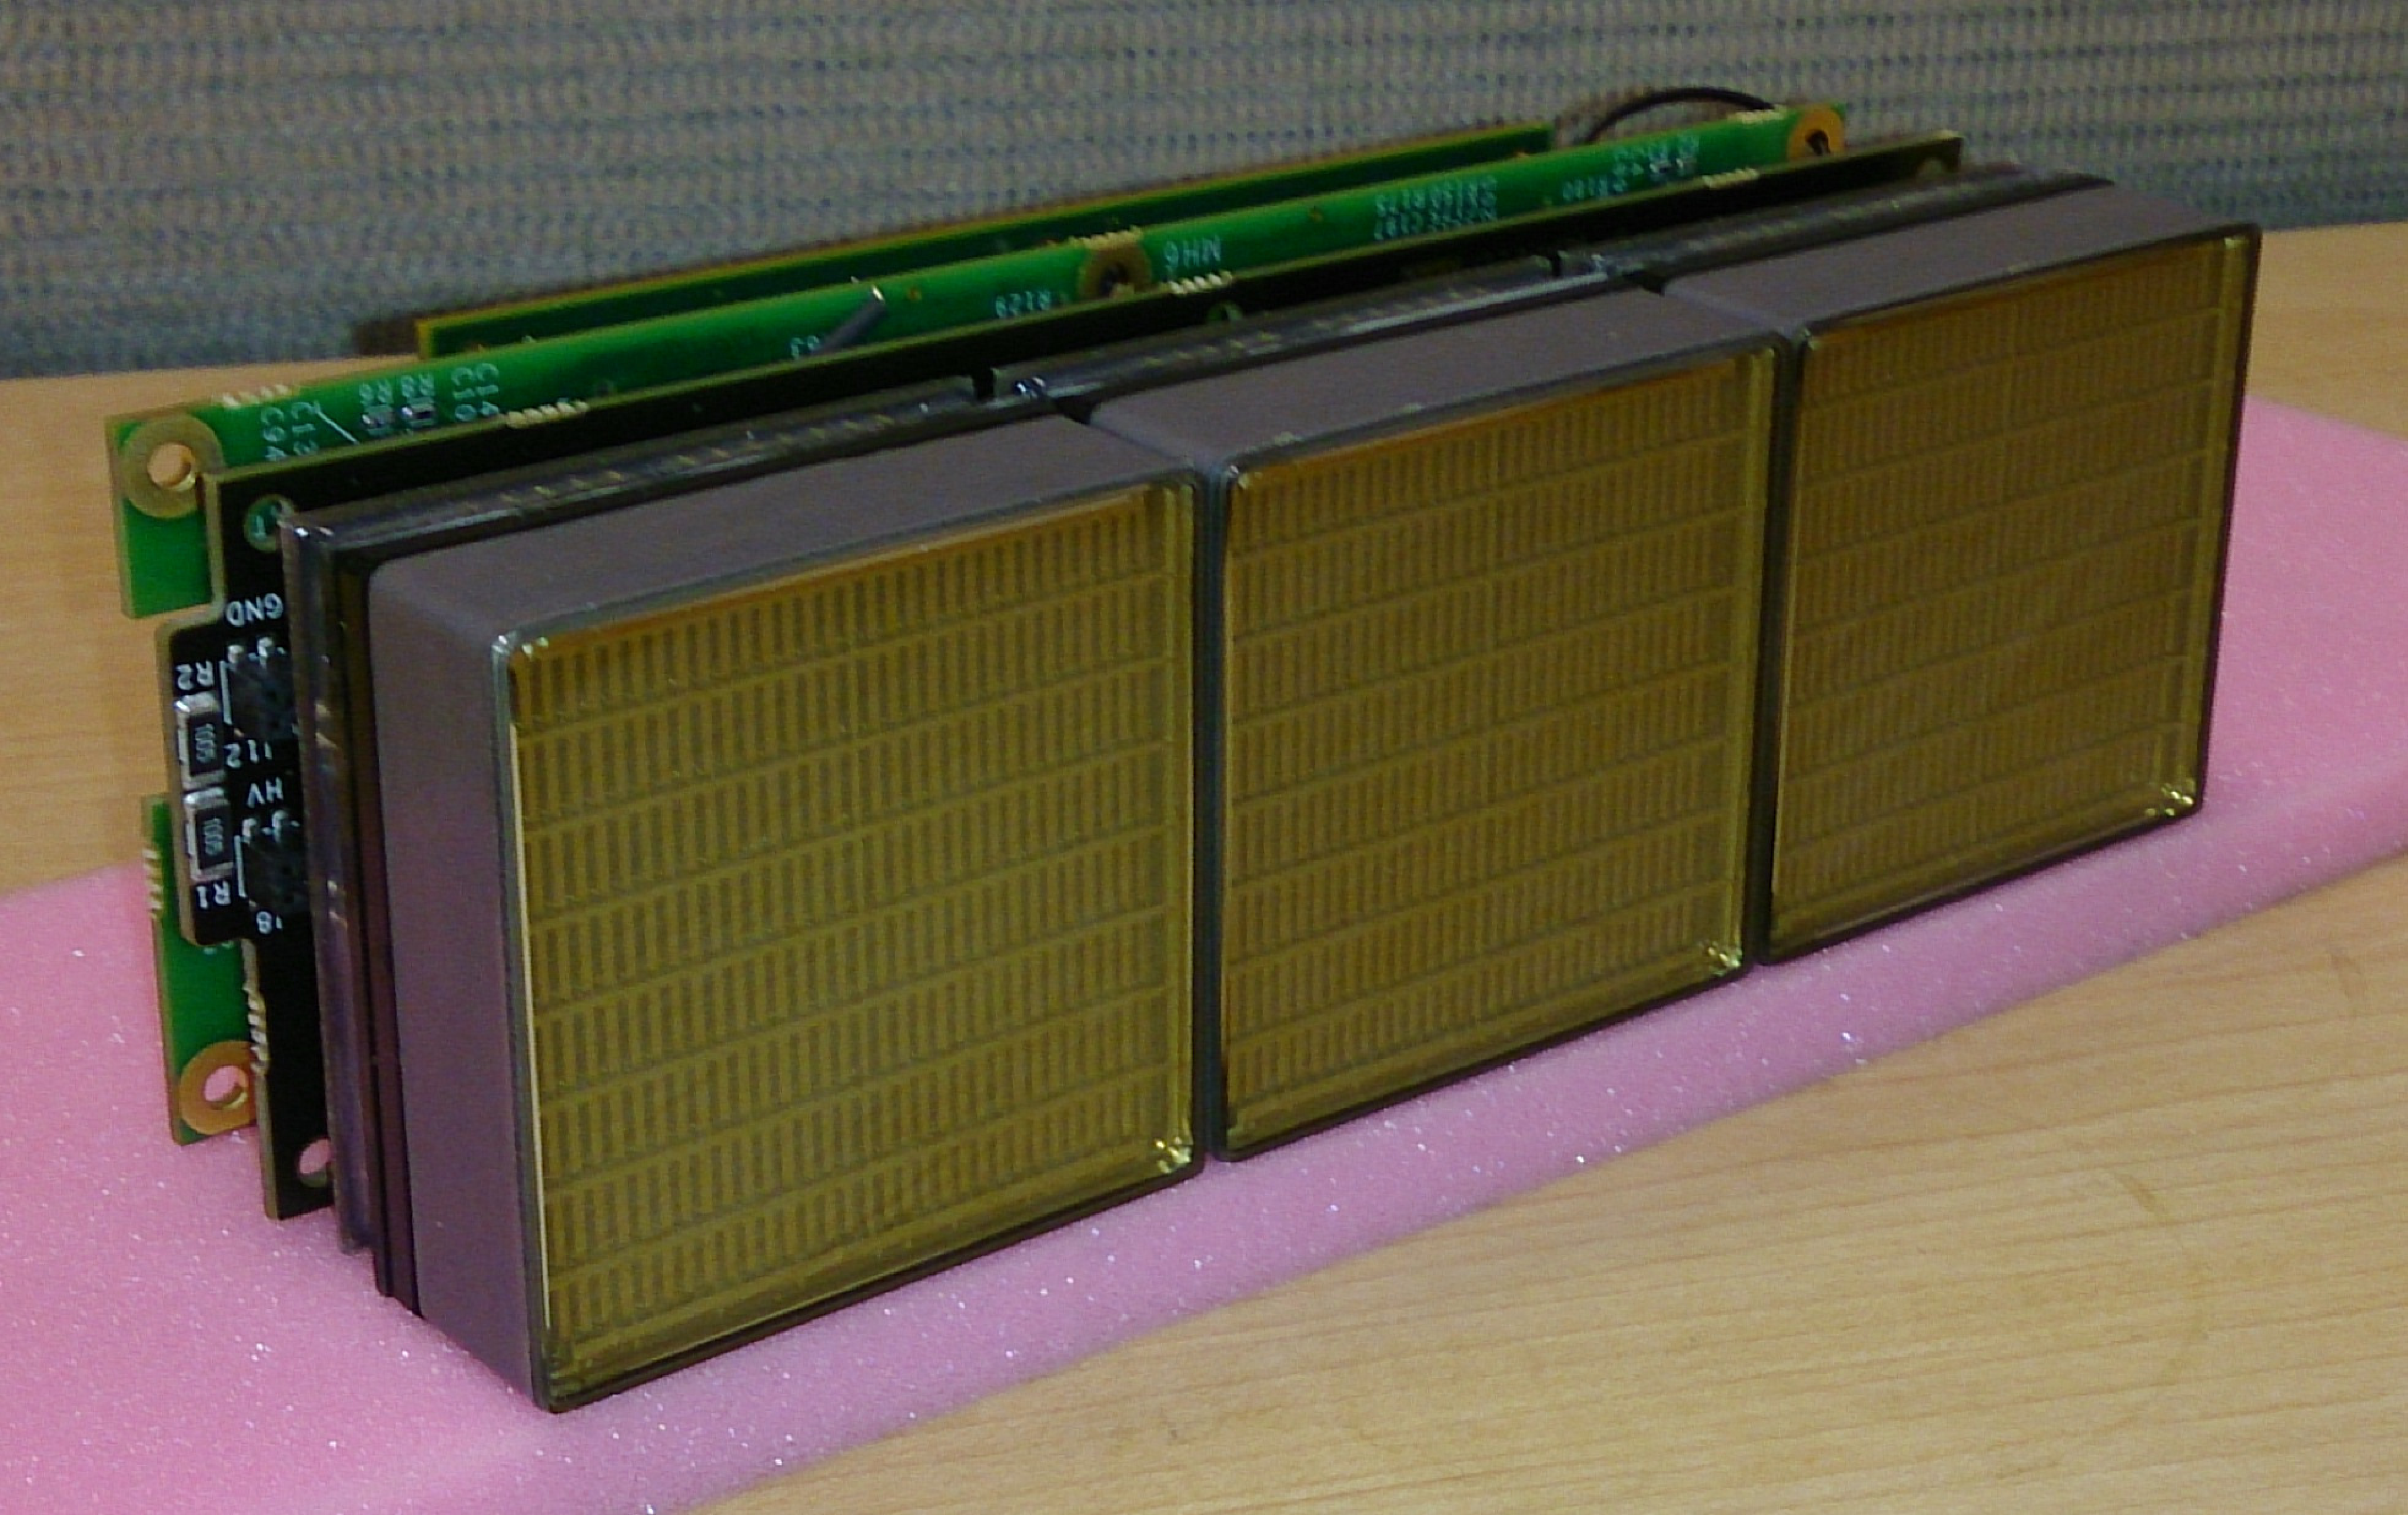
\includegraphics[width=0.8\linewidth]{figures/frontendPMT.pdf}
  \caption{Front-end electronics readout board and mounted MAPMTs.}
  \label{fig:feboards}
\end{figure}

%Each MAROC chip consists of 64 independent channels and is equipped with single channel adjustable preamplifier, configurable signal shaping, slow shaper capable of charge measurements and binary output with fast shaping and adjustable threshold.
%The single channel has a pre-amplification and configurable 8 bit gain correction stage followed by independent binary and analog lines.
%The binary line is digital and most suitable for the RICH application.
%We are planning to analyze the performance of MAROC chip as a function of its threshold and gain.
%Additionally front-end electronics stability and noise will be tested as well.

%The custom modular design as shown on Fig.~\ref{fig:feboards} consists of sandwich architecture where one board hosts the ASIC chips (2 or 3 per board) and another active board hosts the FPGA to manage and configure the ASICs, the third board is a passive adapter for MAPMT sockets.
%The conceptual design of the electronics readout boards was finished in the RICH development phase and currently we have several board implementations available at Jefferson Lab and INFN for final tests.

The measurements of custom front-end electronics together with installed MAPMTs in the RICH Black Box setup were crucial to understand their performance in the RICH detector.
To test and calibrate it multiple tests with internal onboard charge injector, external charge injector and signal generator were performed.
As shown in previous section on Fig.~\ref{fig:MAPMTtest}, RICH MAPMT test setup can house two FE boards inside the black box.
%The focus of the modification was to adapt the test setup in such way that the swap of FE boards would be fast and easy.
%The PCB guidelines were installed inside the black box to ensure easy mounting and dismounting procedure universal for both 2-MAPMT and 3-MAPMT FE modules.
%This requirement exists in light of the future measurements that our group is expected to perform on all FE modules for testing purposes.
%Each FE module is connected to the low voltage power supply to power FPGA and ASIC boards.
The communication between FPGA board and PC is performed using TCP/IP protocol via optical fiber network cable.
%The HV cables, one per each module, supply power for attached MAPMTs.
The Data Acquisition program runs on external PC under Linux OS, configures FPGA and MAROC boards and collects the data through network interface.
%The laser with neutral density filters and light diffuser is installed on a moving platform to allow illumination of individual MAPMTs with different light intensities.
The current setup allows fast evaluation of FE modules with highly automatized procedure which is important because RICH panel consists of 113 tiles with 3-MAPMTs and 23 tiles with 2-MAPMTs FE modules to house 391 MAPMTs.
  	  % Andrey
\section{Maroc chip calibration}

To remove the non-linearity within the ADC readout, a procedure was developed to convert the amplitude of the MAROC slow shaper signal from ADC channels into charge. The MAROC has a built-in charge injection functionality consisting of a test input pin which is connected to the preamplifiers through a logic network of switches and 2 pF capacitors. Together with an external step function generator, this can be used to inject a controllable amount of charge directly into the preamplifiers. We measured the output of the slow shaper in ADC channels for 82 different input charges ranging from 0 to 4 pC. Fig.~\ref{fig:MAROCcalib} shows the relationship between the injected charge and the measured amplitude in units of ADC channels for three different readout channels. The relationship between charge and ADC channels is linear up to about 1.5 pC. This distribution was observed to vary between chips and pixels, and thus a unique distribution was measured for all 64 pixels on each MAROC used in this study. 

\begin{figure}[hbt]
	\centering
	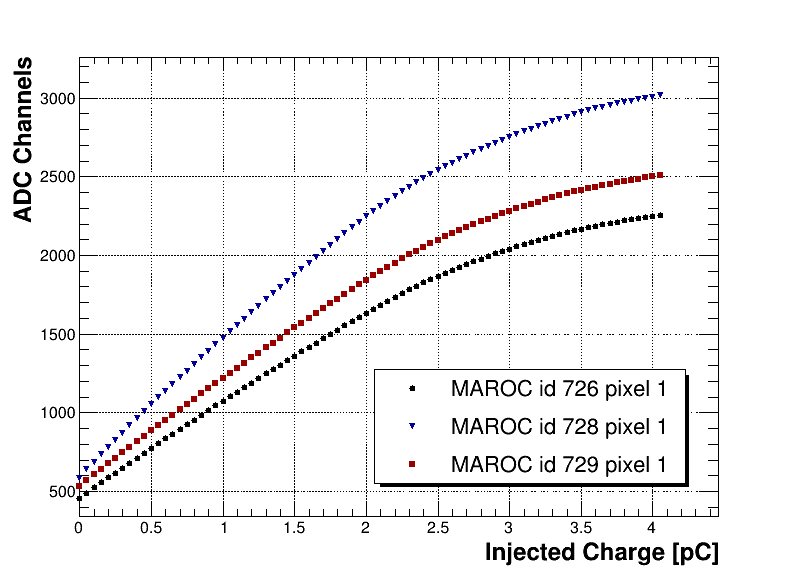
\includegraphics[width=\linewidth]{figures/adc_v_charge.png}
	\caption{Response of MAROC slow shaper in ADC channels as a function of the injected charge. This curve is for MAROC id 726 and pixel 01.}
	\label{fig:MAROCcalib}
\end{figure}

This calibration data was used to convert the measured amplitude in ADC channels into charge collected on an event-by-event basis. The interpolation is done by assigning quadratic functions to every calibration data point to obtain local estimates of the charge as a function of ADC channels. The quadratic functions are obtained by fitting the nearest 5 data points, so that the value of the function is not constrained to equal the measured ADC channels at the given injected charge. For each event, the charge is estimated as a linearly weighted average between the extrapolations of the quadratic functions from the nearest two data points. Fig.~\ref{fig:H12700calib} and Fig.~\ref{fig:H8500calib} show typical amplitude distributions before and after this conversion is applied for one H12700 MAPMT pixel and one H8500 MAPMT pixel, respectively. For both, the conversion to charge extends the high-amplitude tails of the spectra due to the nonlinearity of the ADC readout.

\begin{figure}[hbt]
	\centering
	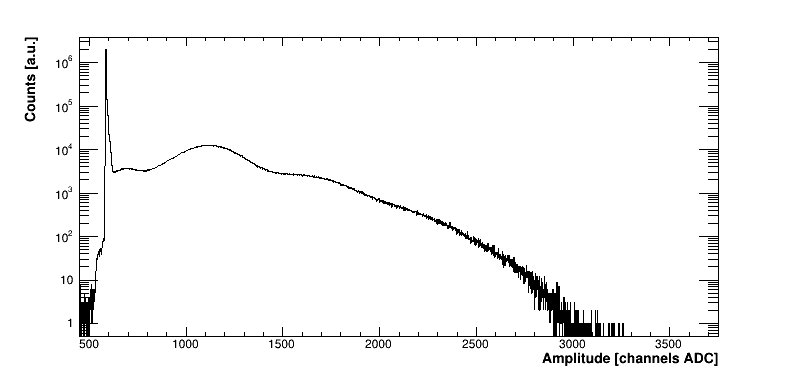
\includegraphics[width=\linewidth]{figures/GA0982_w1_g064_v1100_063_adc.png}
	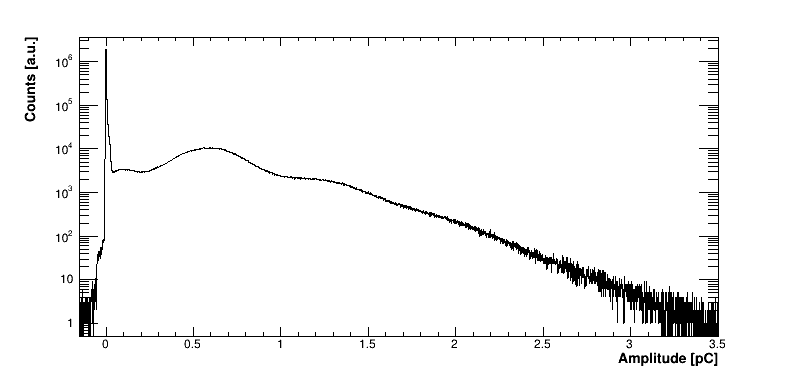
\includegraphics[width=\linewidth]{figures/GA0982_w1_g064_v1100_063_pC.png}	
	\caption{Top: A typical spe spectrum for one HA12700 pixel in units of ADC channels. Bottom: The same spectrum after converting the units into pC.}
	\label{fig:H12700calib}
\end{figure}

\begin{figure}[hbt]
	\centering
	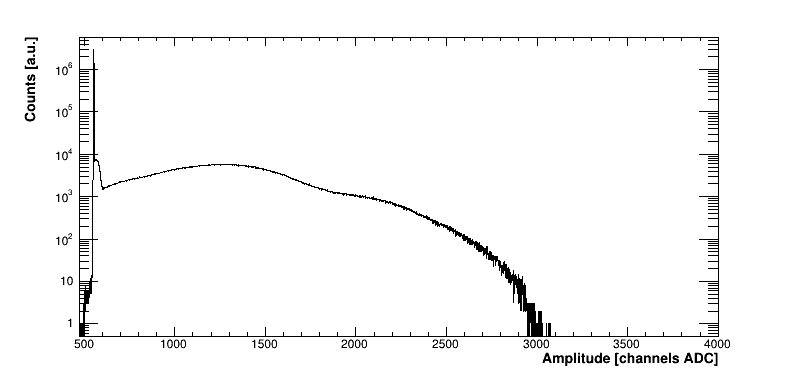
\includegraphics[width=\linewidth]{figures/CA7811_w1_g064_v1100_056_adc.png}
	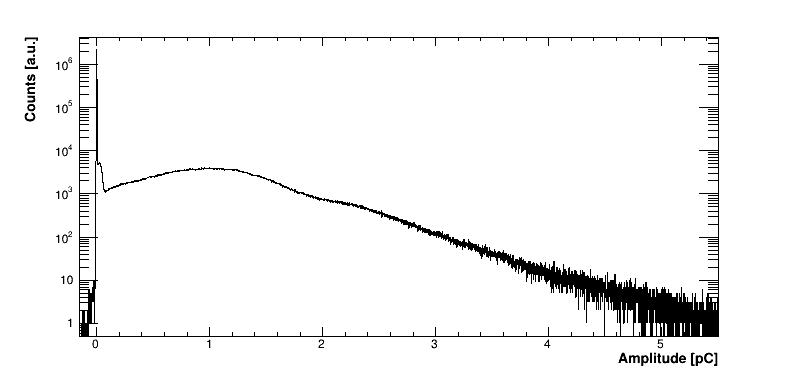
\includegraphics[width=\linewidth]{figures/CA7811_w1_g064_v1100_056_pC.png}	
	\caption{Top: A typical spe spectrum for one HA8500 pixel in units of ADC channels. Bottom: The same spectrum after converting the units into pC.}
	\label{fig:H8500calib}
\end{figure} % Drew
\section{Cross talk measurements}

To demonstrate the crosstalk between adjacent pixels on the MAPMTs, we collected data where the whole PMT face was masked with a sheet of black paper, and a single 3mm diameter hole was punctured over the center of one pixel. Despite the majority of the laser light being incident on the single unmasked pixel, we observed signals above pedestal in the surrounding pixels as well. Fig.~\ref{fig:H12700pinhole} shows the measured spectra for the central and neighboring pixels when the puncture hole was directly above pixel 29. There are two types of events we see in this data set for the pixels surrounding the illuminated pixel. The first is the electronic crosstalk resulting from the electron cascade in the central pixel. The signal measured in a neighboring pixel is directly proportional to that which is measured in the central pixel. In Fig.~\ref{fig:H12700pinhole}, these types of events are characterized by a shoulder attached to the right of the pedestal. This is most prominently seen in the spectrum for the pixel directly to the right of the central pixel of Fig.~\ref{fig:H12700pinhole} (pixel 30). Because of the strong correlation of the crosstalk to the central pixel, these types of events can be identified and removed from the data offline. More will be discussed on this later.

The second type of event observed in the neighboring pixels of this data comes from the displacement of the photoelectron emitted by the photocathode. When the incident photon hits pixel 29, there is some probability that the emitted photoelectron is detected by one of the neighboring pixels. Because there is no correlation with the central pixel for these events, there is no way to identify these signals on an event-by-event basis. In Fig.~\ref{fig:H12700pinhole}, the spectra drawn in red have the additional cut applied that the signal in the central pixel should be greater than 10$\sigma$ above the pedestal. With this cut applied, the number of events beyond the crosstalk shoulder in the neighboring pixels is reduced by more than an order of magnitude.

\begin{figure}
	\centering
	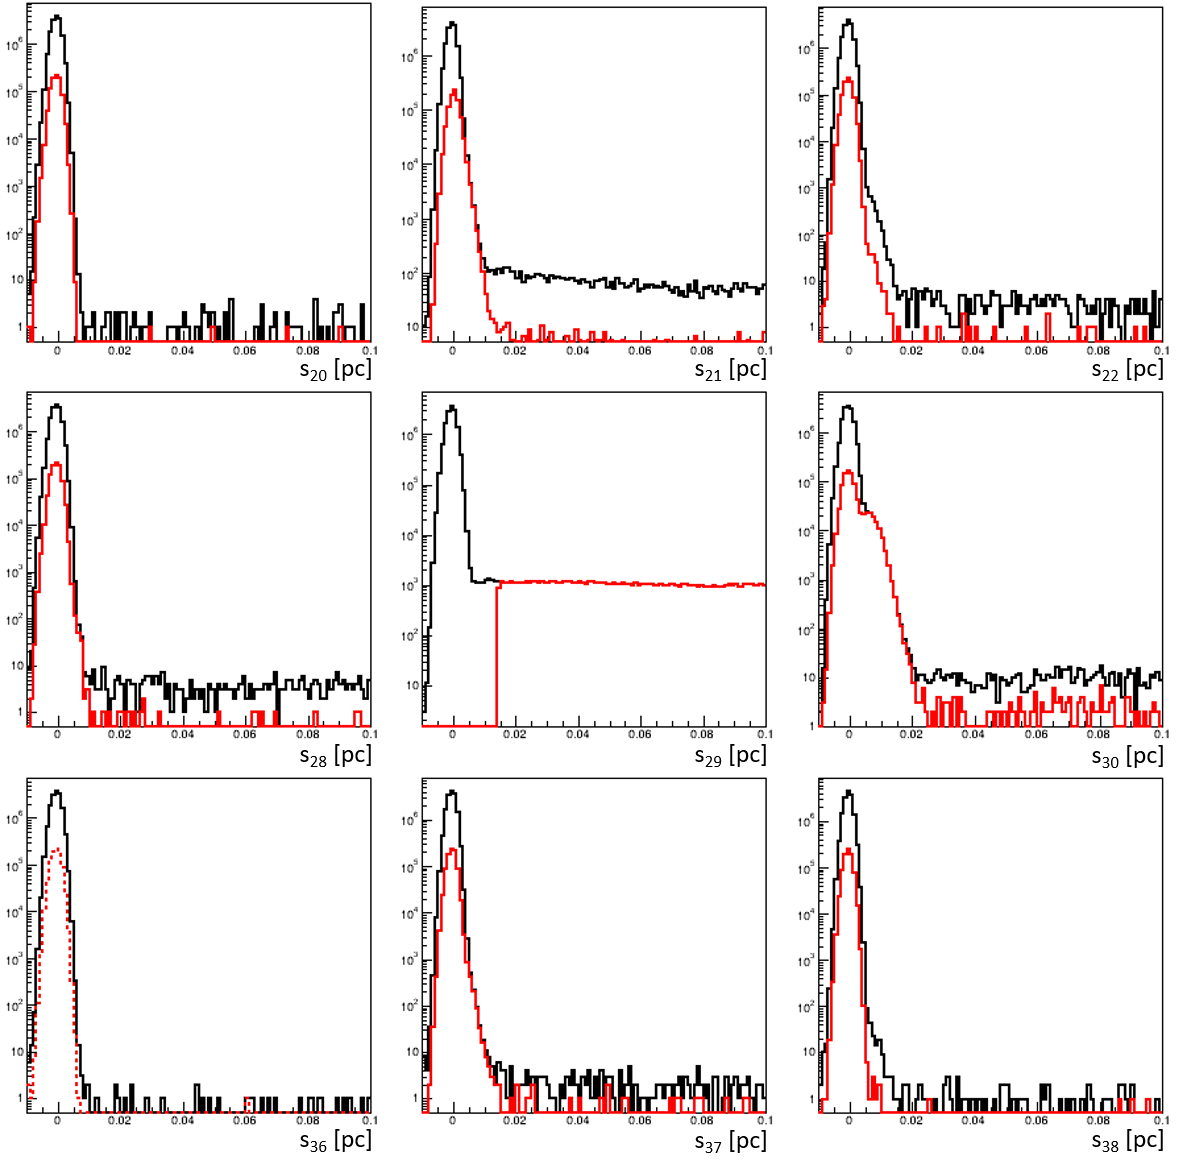
\includegraphics[width=\linewidth]{figures/H12700_3mm_mask_config5_ct.png}
	\caption{Black: the charge spectra for pixel 29 of a typical H12700 MAPMT and the surrounding pixels when only pixel 29 was illuminated by the laser light. Red: the same spectra with the cut that the signal in pixel 29 is 10$\sigma$ above pedestal.}
	\label{fig:H12700pinhole}
\end{figure}

Using this masking scheme, we collected data with different pixels unmasked and measured the fraction of events where we observe cross talk in the neighboring pixels. Fig.~\ref{fig:H12700_ct_ratio} shows these fractions for four pixels. 

\begin{figure}
	\centering
	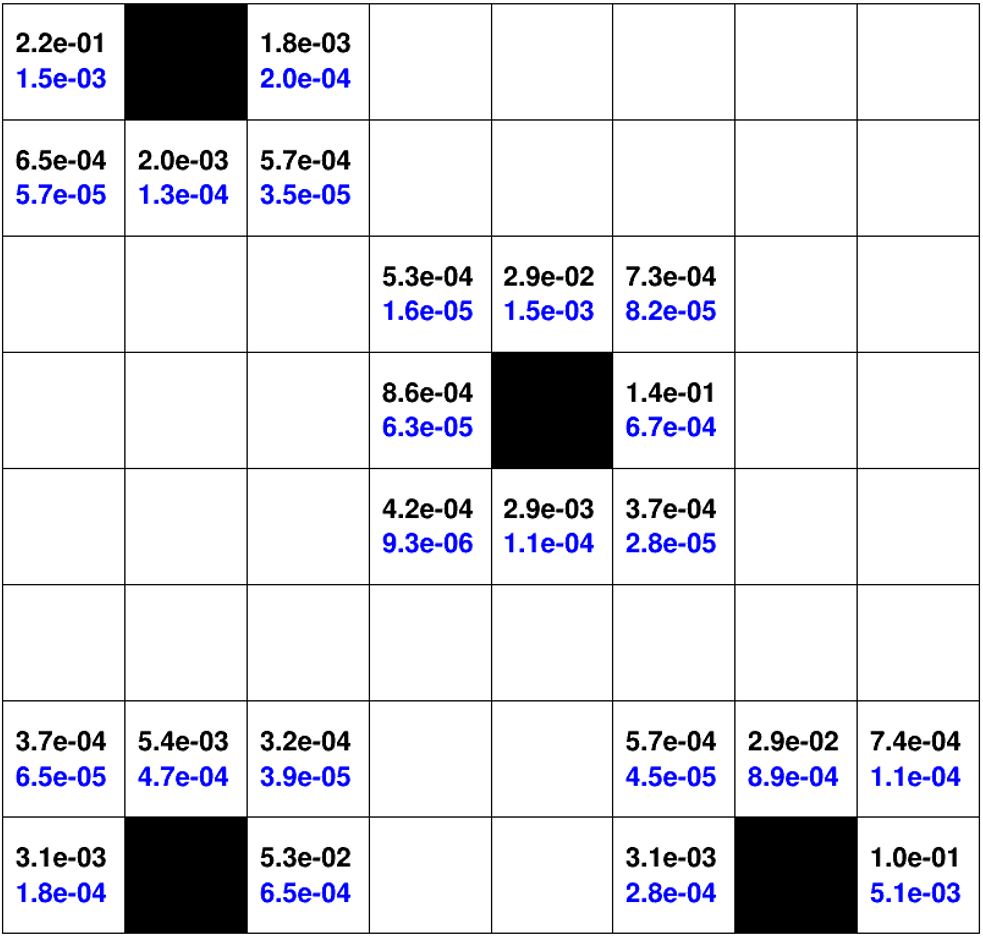
\includegraphics[width=\linewidth]{figures/H12700_ct_ratio.png}
	\caption{For each highlighted pixel a separate run was taken where only this pixel had a 3mm hole punctured in the mask covering the whole PMT face. The numbers in black in the surrounding pixels represent the fraction of events where there is crosstalk in that pixel.}
	\label{fig:H12700_ct_ratio}
\end{figure}

To properly characterize the single photoelectron spectrum for each pixel, one needs to either add a description of the crosstalk into the computational model for the s.p.e. response, or one can attempt to identify and remove these crosstalk events from the data. A simple procedure was developed and implemented to attempt the latter option. Because the amplitude of the crosstalk is linearly dependent on the amplitude of the photo-induced signal, the crosstalk events appear as linear bands in the plots showing the measured charge in one pixel as a function of the measured charge in a neighboring pixel. Fig.~\ref{fig:H12700neighbors} and Fig.~\ref{fig:H8500neighbors} show these two dimensional plots for all pixels which neighbor pixel 29 for one H12700 MAPMT and one H8500 MAPMT, respectively. The data shown in these plots were taken with the entire face of the MAPMTs illuminated by the laser light. From these two plots it is obvious that the strength of the crosstalk is vastly different between the H12700 and H8500 MAPMTs. On average, the amplitude of the crosstalk in an H12700 MAPMT is only about 2-3$\%$ of the main signal, whereas the crosstalk amplitude in an H8500 MAPMT can be as large as 50$\%$ of the main signal. As we will discuss later, this fact makes it more difficult to address the crosstalk for the H8500 MAPMTs in the mathematical description of the spe response function.

Other noteworthy features from Fig.~\ref{fig:H12700neighbors} and Fig.~\ref{fig:H8500neighbors} are that the crosstalk signals are strongest in the pixels immediately to the right and left of the pixel where light was incident. The crosstalk bands in those pixels have the largest slope. Most of the crosstalk is contained within the 4 pixels which share an edge with the illuminated pixel, as the plots for the pixels on the corners show little correlation with the charge measured in the central pixel.

\begin{figure}[hbt]
	\centering
	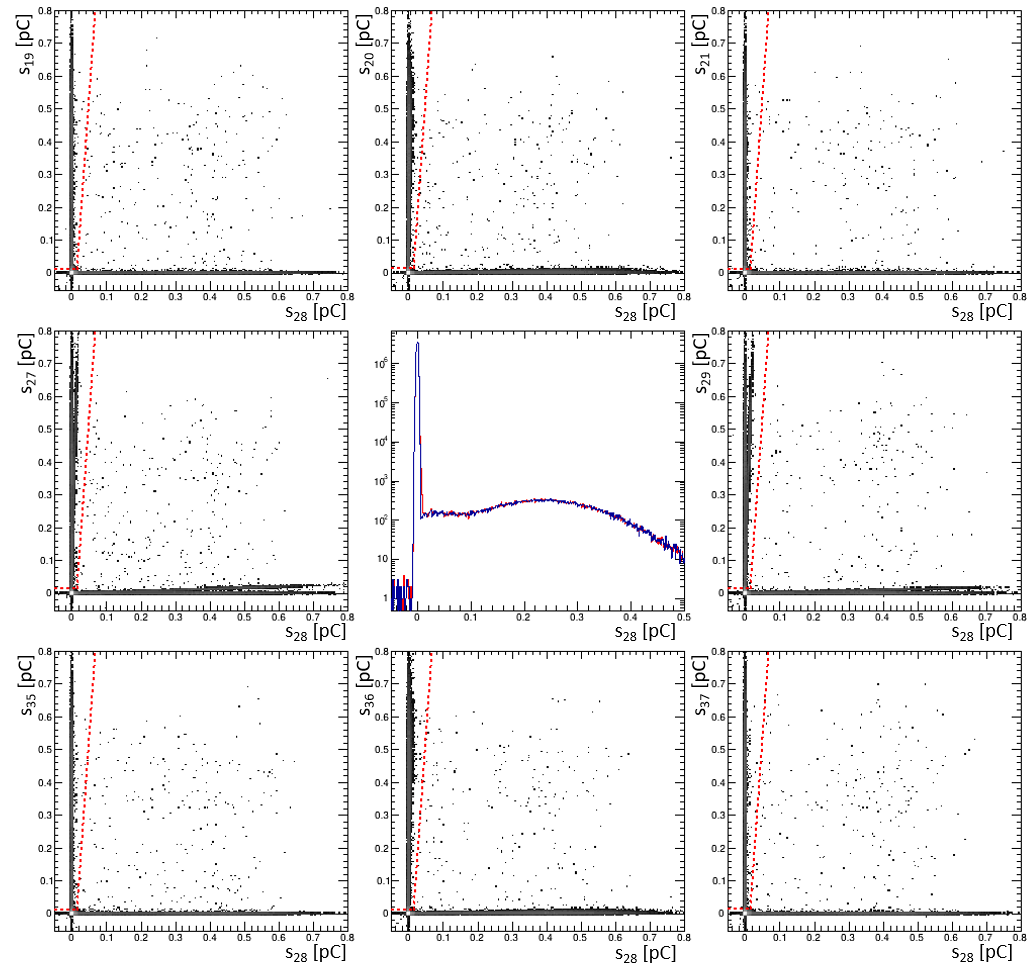
\includegraphics[width=\linewidth]{figures/H12700_ct.png}
	\caption{The charge measured in adjacent pixels is plotted as a function of the charge measured in pixel 29 for a typical H12700 MAPMT. The central plot shows the charge spectrum before (red) and after (blue) removal of the crosstalk events which are cut by the dashed (red) line on the 2-dimensional plots.}
	\label{fig:H12700neighbors}
\end{figure}
\begin{figure}[hbt]
	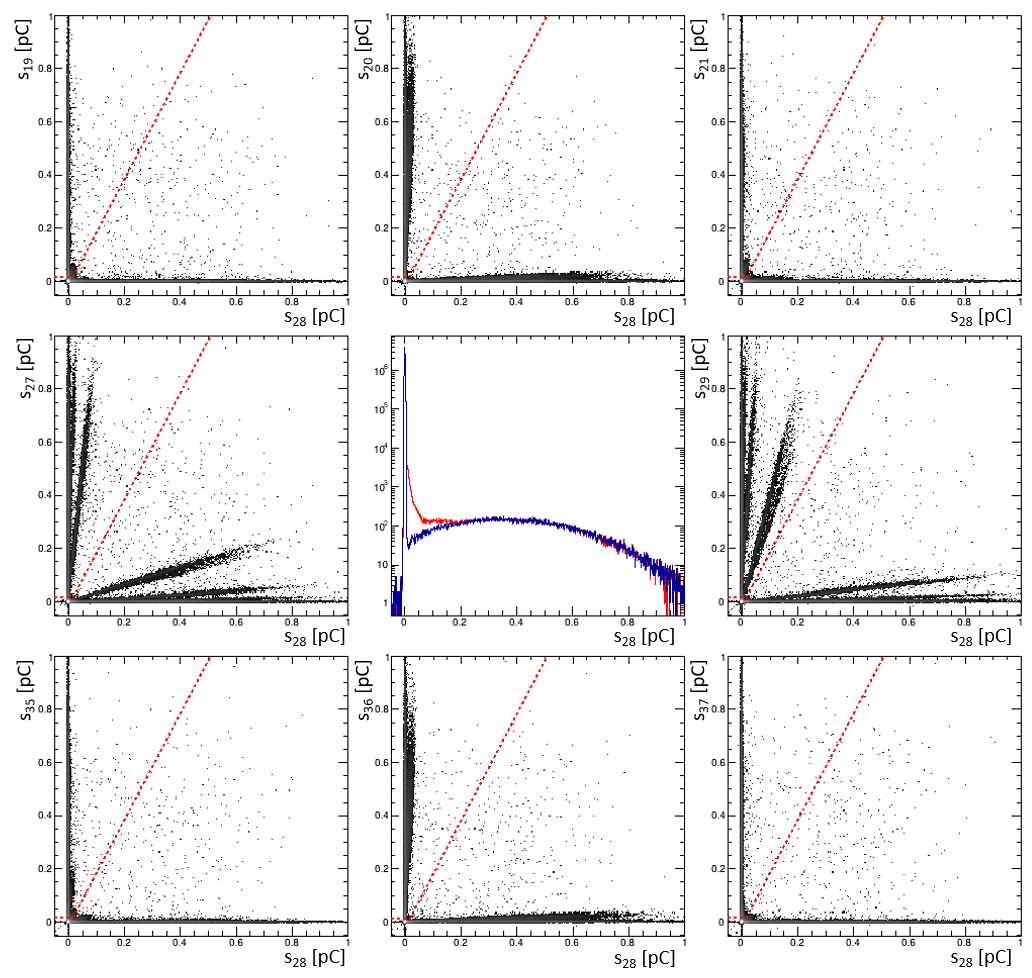
\includegraphics[width=\linewidth]{figures/H8500_ct.png}
	\caption{The charge measured in adjacent pixels is plotted as a function of the charge measured in pixel 29 for a typical H8500 MAPMT. The central plot shows the charge spectrum before (red) and after (blue) removal of the crosstalk events which are cut by the dashed (red) line on the 2-dimensional plots.}
	\label{fig:H8500neighbors}
\end{figure}

Because the crosstalk events are easily distinguished in these two dimensional plots, a cut can be placed to remove these events from the data. The cut is applied to each pixel separately, and is a linear function of the charge measured in that pixel. Specifically, the cut places a limit on the maximum charge measured in the neighboring pixels. If the maximum neighboring charge is above the cut value for the central pixel\textquotesingle s measured charge, then the event is tagged as crosstalk and is removed from the charge spectrum for the central pixel. This cut is shown as a dashed (red) line in Fig.~\ref{fig:H12700neighbors} and Fig.~\ref{fig:H8500neighbors}. The start of the cut line is placed 7$\sigma$ above the pedestal to avoid removing pedestal events. Although the slope of the crosstalk bands can vary between pixels, the slope of the cut line used here is the same for each pixel on a given PMT. 

The main drawback of this crosstalk cut is that it removes events where adjacent pixels both happen to have a photoelectron emitted from the same laser trigger. However, the fraction of these accidental coincidence events is low when the laser filter is used at the minimal setting, meaning at low light intensity this procedure can be used to provide the spe spectrum free from electronic crosstalk. The charge spectra before and after the removal of the crosstalk events in this manner is compared in the central plot in Figs.~\ref{fig:H12700neighbors} and~\ref{fig:H8500neighbors}. For both the H12700 pmt and the H8500 the crosstalk shoulder to the right of the pedestal is removed after applying this cut. 
		  % Drew
\section{Calibration of laser photon flux}

The calibration of the absolute laser photon flux was performed with the use of the silicon photodiode  Hamamatsu S2281.
The tabulated quantum efficiency of this diode at the wave length of our laser ($\lambda=470$ nm) is 62.6\%. 
The active part of the diode is a circle with a diameter of 11.3 mm, which is 100 mm$^2$. 
The picoammeter KEITHLEY 6485 was used to measure the average diode current while illuminated by the laser beam.
The noise diode current was estimated to be at the level of 0.2 pA. 
During the MAPMT characterization, the laser frequency was maintained at 20 kHz. 
For light calibration, the higher the frequency, the better current measurement accuracy may be achieved from point of view the noise level. 
The maximum frequency of our laser is 1 MHz.
However, there are additional systematic uncertainties associated with the extrapolation from one frequency to another. 
For this reason, the scan of the light field was done at a working frequency of 20 kHz. 
The measured current in the center position of the laser head was around 29.2 pA at this frequncy, meaning the systematic unsertainty
of this measurement was below 1\%.  We made a detailed 2D scan of the photon flux by
moving the laser head with step sizes of 2 mm in the X and Y directions along the full area where the 3 MAPMTs were located during the characterization procedure.
Normalized to one laser pulse and one mm$^2$ area, the number of photons with $\lambda=470$ nm  is presented in Fig.~\ref{fig:light_flux}.
The maximum value of the photon flux in the center of the light field equals 145 $\gamma/mm^2/pulse$.
These measurements were done without  any optical filters installed. We used neutral density calibrated optical filters with antireflection coating.
To check the possible filter effects we made a measurement of the light flux for one of the filters with a tabulated attenuation of 100. 
This test was done with a frequency of 1 MHz to increase the accuracy of the current measurement. 
The ratio of the measured attenuation factor to the tabulated one was determined to be 1.05$\pm 0.01$. This coefficient was applied to the map of the photon flux when used for data with optical filters. It takes into account the possible effects of rescattering or reflection of the photons by filters.
\begin{figure}[h]
\centering
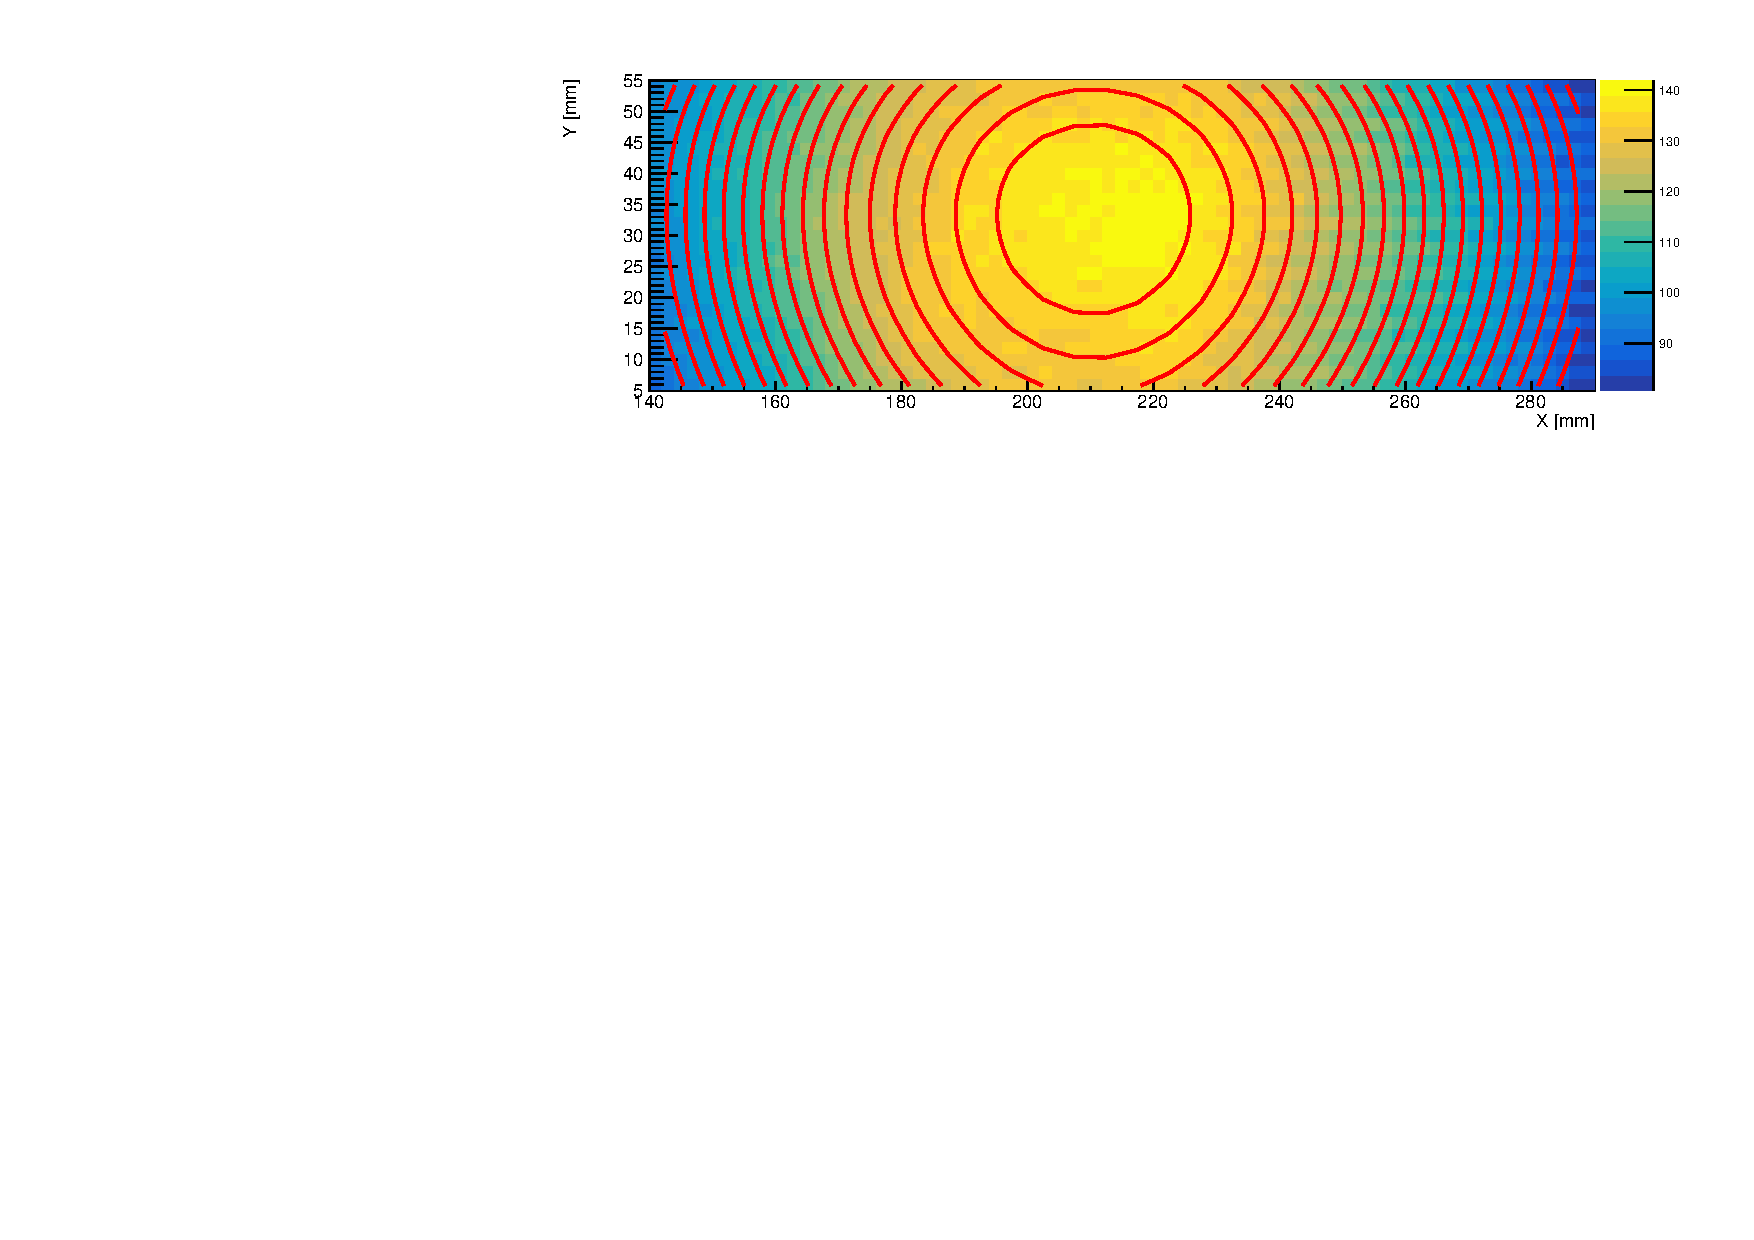
\includegraphics[width=0.5\textwidth]{figures/photon_flux.pdf}
\caption{Number of photons per mm$^2$ in  one laser pulse.}
\label{fig:light_flux}
\end{figure}

The knowledge of the absolute number of photons hitting the photomultiplier tubes during the characterization gave us the possibility to measure the quantum efficiency of the MAPMTs for each pixel. The average number of photoelectrons, $\mu$, is proportional to the quantum efficiency:
$$
\mu=\epsilon_{Q.E.} \int_{S_{pixel}}\frac {dN_\gamma}{dS} dS
$$
\noindent
where $\int_{S_{pixel}}\frac {dN_\gamma}{dS} dS$ is the number of photons integrated over the pixel's area, $S_{pixel}$, and $\epsilon_{Q.E.}$ is the quantum efficiency of the pixel.
Integration included the measured light field at the position of the pixel under study.
The parameter $\mu$ was determined during the PMT characterization. % Drew
\section{Mathematical model for the description of the PMT's response}

The goal for using MAPMTs in RICH detectors is to achieve reliable detection of single photons in the Cherenkov light radiation cones. Single photon incident on a PMT face may knock out a single photoelectron from the PMT's photocathode with a certain probability, defined as Quantum Efficiency (QE). The photoelectrons cascade inside the PMT to generate a typical amplified electrical signal at the anode. The amplitude distribution of the single photoelectron (SPE) signals depends on the PMT design and high voltage applied, and varies from pixel to pixel. Tests and characterization of multiple MAPMTs include measuring the SPE amplitude distributions for every pixel, finding out the appropriate amplitude thresholds, and determining QE. To achieve this goal we used the methods developed in ~\cite{DEGTIARENKO20171}, expanded to include the new empirical method to take into account the effects of pixel-to-pixel cross talk in the H12700 tubes. The reference ~\cite{DEGTIARENKO20171} describes in detail the mathematical model used to extract and parametrize the SPE distributions from the measurements using the test setup. The method allows in principle to describe the SPE functions of essentially any complexity by decomposing them as a sum of Poisson distributions with different averages. For the detailed explanations and the definition of the model parameters please refer to ~\cite{DEGTIARENKO20171}. The list of main parameters includes $\mu$, average number of photoelectrons produced by the laser in a given pixel per one pulse, and {\it{scale}}, average amplitude of the SPE distribution in pC. Five parameters determine the shape of the SPE distribution, defined as a normalized sum of three Poisson distributions with different average multiplication coefficients applied to the photoelectron on the first dynode of the PMT. Average multiplication on the first cascade ${\nu}$ may be derived from these parameters. ${\sigma}$ parameter describes the Gaussian shape of the pedestal function. ${\xi}$ parameter describes effective cascade multiplication on the second dynode. The combination of 9 parameters describes a single-anode PMT SPE response in an ideal measurement setup with a Gaussian pedestal function. If the pedestal amplitude distribution is not exactly following the Gaussian shape the problem of parameterizing the SPE distribution requires addition of new parameters taking into account the distortion of the pedestal Gaussian. The method was successfully implemented in ~\cite{DEGTIARENKO20171} in the case of small exponential noise contribution to the Gaussian measurement function, see the Eqs. (38-40) in that publication. In the present study we attempt to use similar approach to parametrize and approximate the contribution of the crosstalk signals coming from the neighboring pixels to the SPE amplitude distribution. The model for the process, in agreement with the observations presented in the previous chapter, assumes that a portion of the signal from a neighboring pixel may be randomly added to the amplitude measured in a given pixel under investigation. Such random contribution could in principle depend on the neighbor. It would be impossible to characterize all possible pair combinations. The ad hoc approximation implemented in this work assumes that the spectral shape of the crosstalk contribution is relatively small compared with the average SPE amplitude, and can be averaged over all neighbors and parameterized using three parameters characterizing generally Poissonian shape of the crosstalk spectrum from an average "neighbor event" when the photoelecton signal in the neighboring pixel generates it. Such addition may be considered an addition to the Gaussian measurement function, similar to how it was  


 
We started by using a model for signal amplitude distribution based off of Gaussian single photoelectron spectra as discussed in \cite{Bellamy:1994bv} that works reasonably well for H8500, but this model does not satisfactorily treat the spectra seen in the new H12700 MAPMTs from Hamamatsu. Consequently, Pavel Degtiarenko~\cite{DEGTIARENKO20171} has developed a more complicated model using several Poisson components to better fit the MAPMT spectra, especially in the single photoelectron cases.
This mathematical model features a realistic description of the MAPMT response where each parameter corresponds to the physical process inside the MAPMT.
The SPE spectrum is fitted with a function used to describe the signal amplitude distribution measured by the MAPMT as shown on Fig.~\ref{fig:SPEfit},
The probability of an initial photon to knock out a photoelectron is distributed according to the Poissonian $P(m;\mu)=\frac{\mu^me^{-\mu}}{m!}$.
To approximate the performance of the first amplification cascade of the MAPMT the function $T(n,m;t)$ is introduced in the model as trinomial sum of three Poissonians with different average secondary multiplicities and the corresponding three relative probabilities for every photoelectron to generate secondary electrons.
The function $G(a,n;\sigma)$ corresponds to the realistic DAQ measurement function to introduce the experimental resolution into the resulting model function.

\begin{figure}[bt]
	\centering
	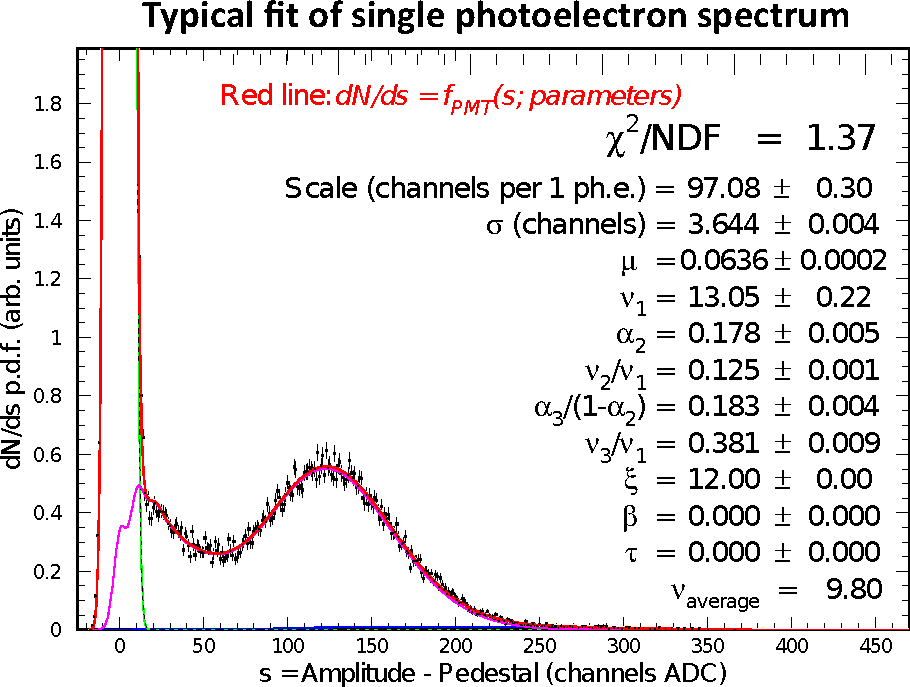
\includegraphics[width=\linewidth]{figures/SPEfit.pdf}
	\caption{Sample of single photoelectron spectrum from one of the pixels at 1000 V with low intensity laser light source,
where integer $m$ corresponds to the number of photoelectrons created at the first stage of the photodetector (photocathode) by the incident light during one event of radiation, index $n$ corresponds to the number of electrons generated at the second stage of the photodetector (first dynode).
}
\label{fig:SPEfit}
\end{figure}

The model is found to describe well the amplitude distributions measured at different levels of radiation with different supply voltages.
The parameters provide MAPMT characteristics independently of the test measurement conditions (see Fig.~\ref{fig:PavelPassport}): the $scale$ parameter is virtually independent on the light radiation level while strongly dependent on high voltage supply, the exact behavior one would expect from the characteristic of internal dynode system of MAPMT.

\begin{figure}[t]
	\centering
	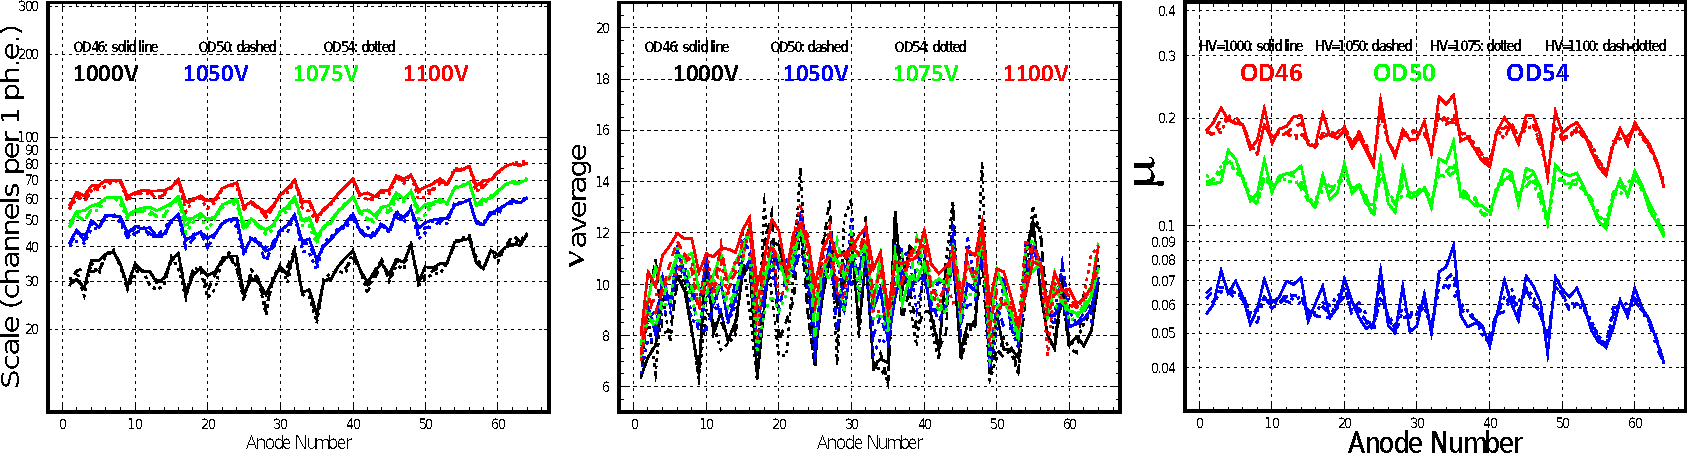
\includegraphics[width=\linewidth]{figures/PavelPassport.pdf}
	\caption{Distributions of fit parameters among the pixels for measurements with 4 different high voltage supplies and 3 different light intensities: the parameter $scale$ characterizes the amplification (dynode) system, $\nu$ - first dynode performance, $\mu$ relates to the quantum efficiency (photocathode performance).}
	\label{fig:PavelPassport}
\end{figure}

Currently we have tested 80 H8500 and 260 H12700 (the largest collection of these new MAPMTs in the world).
The accumulated data provide an immense knowledge about quantum and collection efficiencies of MAPMTs, their surface uniformity, single photoelectron (SPE) spectrum resolution etc.
This parameterized information extracted from the fit of each pixel for every MAPMT is used to describe the detector response in the future simulation.


\begin{figure}[t]
	\centering
	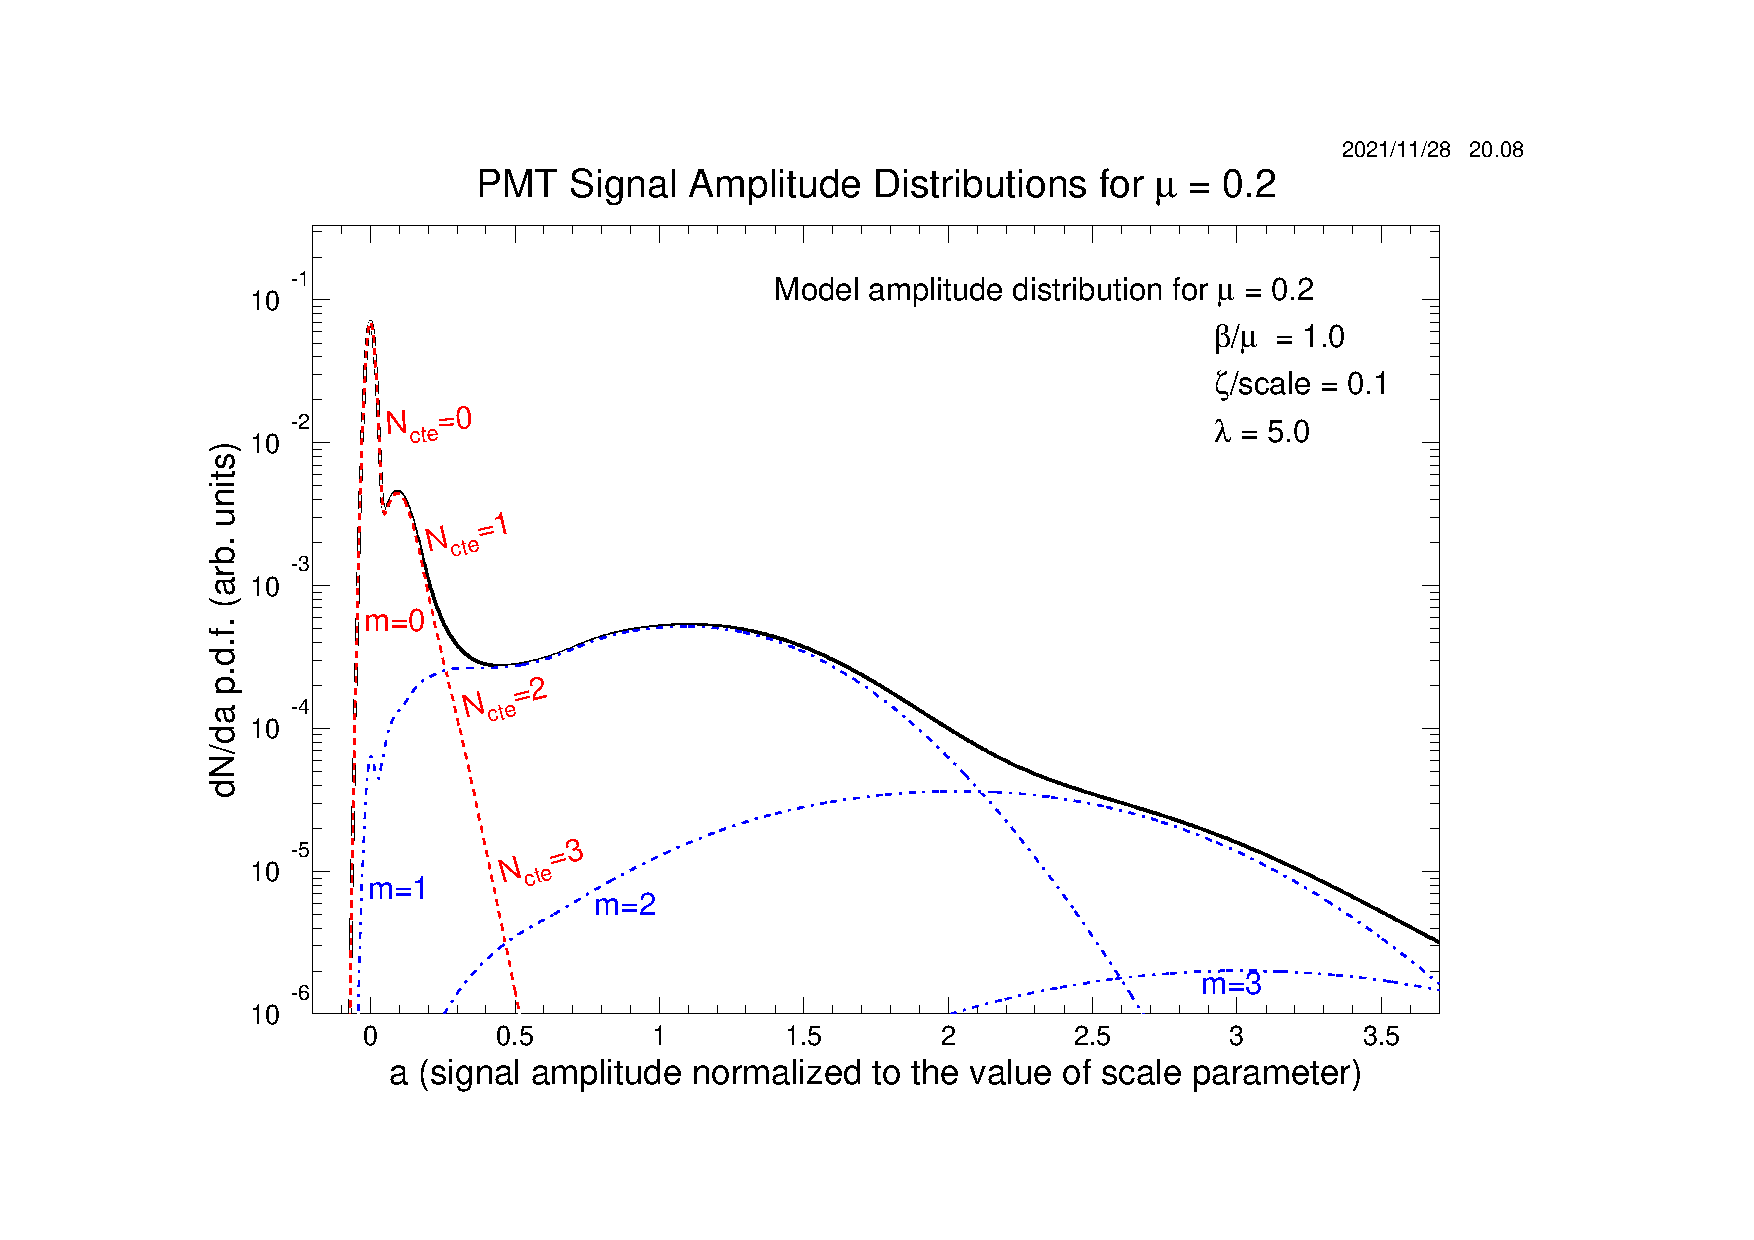
\includegraphics[width=\linewidth]{figures/model.pdf}
	\caption{}
	\label{fig:Model}
\end{figure}		  % pavel
\section{Characterization of MAPMTs}

\begin{figure*}[hbt] 
\centering 
  \subfloat[3 mm mask]{%
    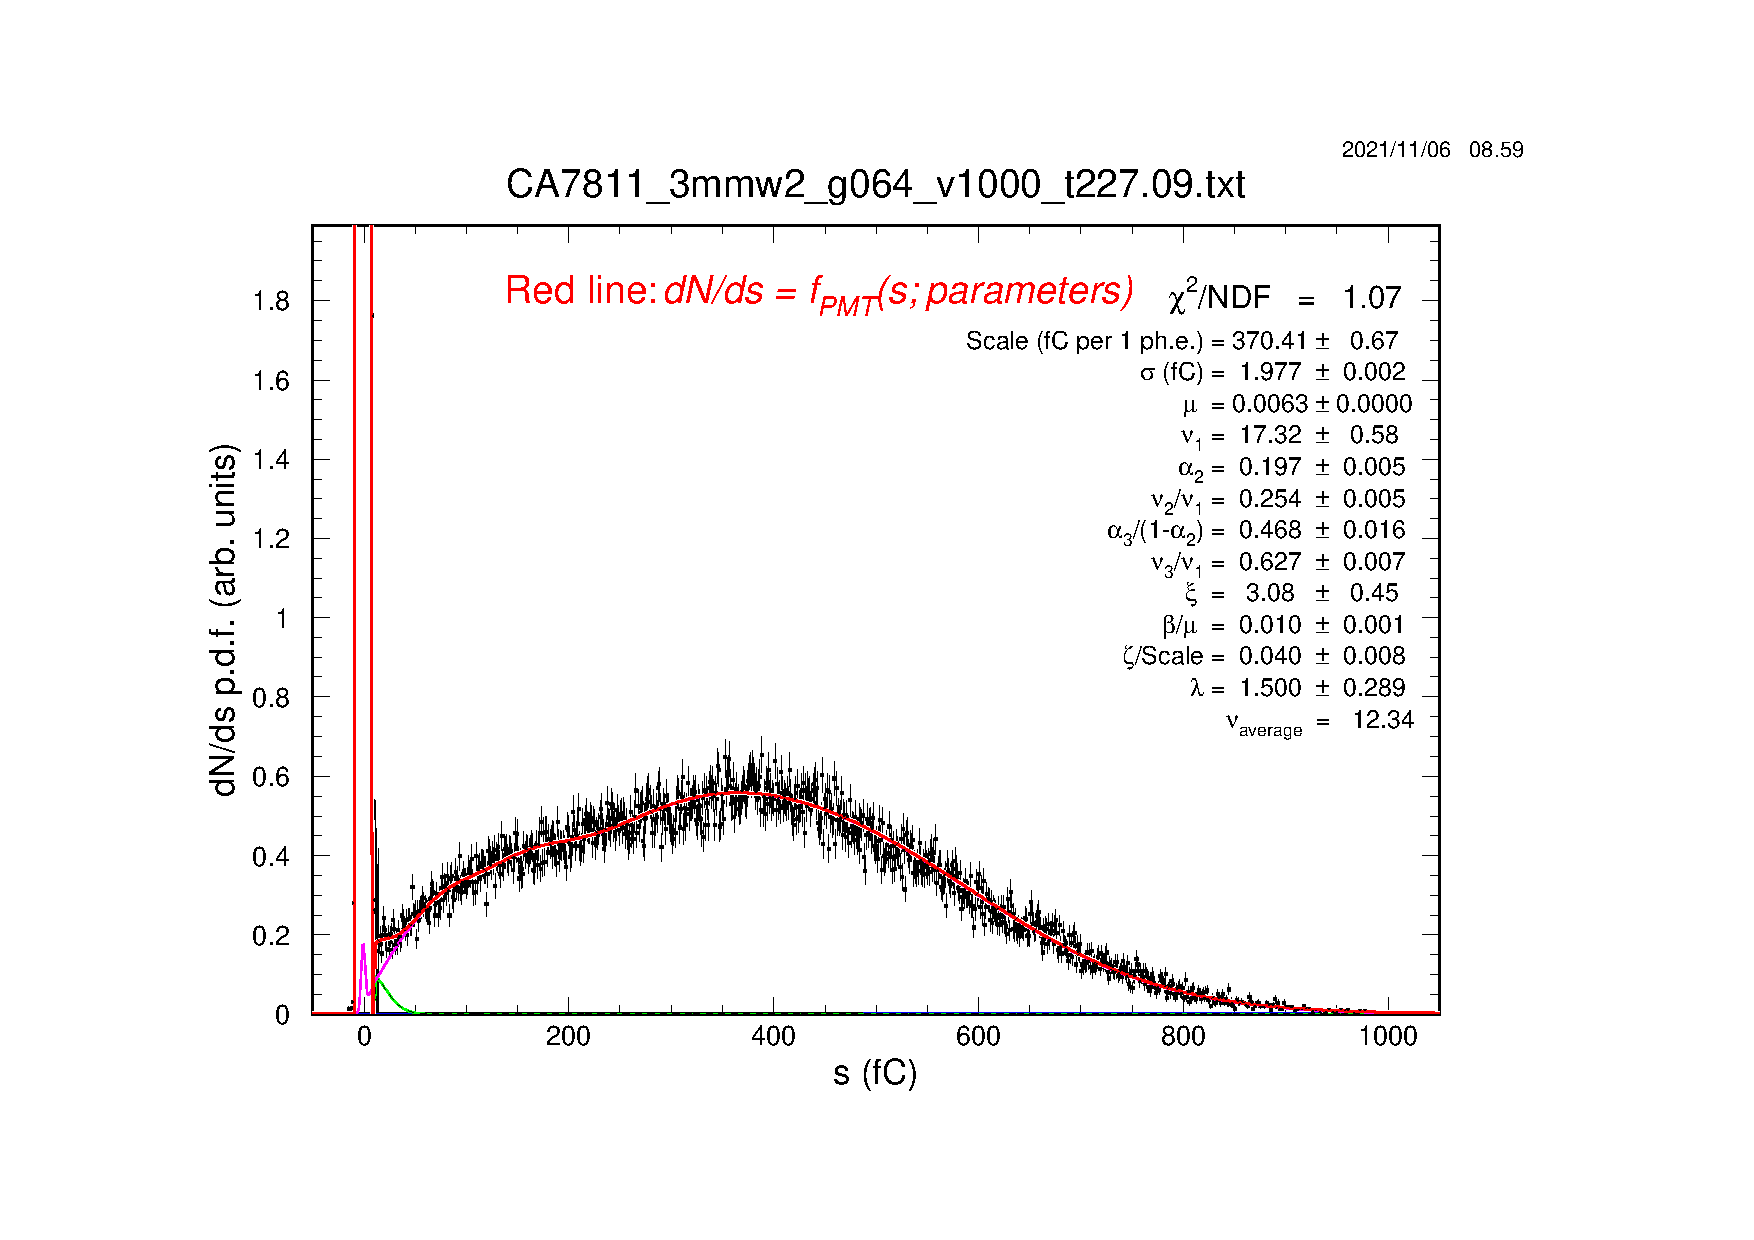
\includegraphics[clip=true,trim=100 75 140 100,width=.49\textwidth,height=.25\textwidth]
                    {figures/CA7811_a.pdf}}
  \subfloat[6 mm mask]{%
    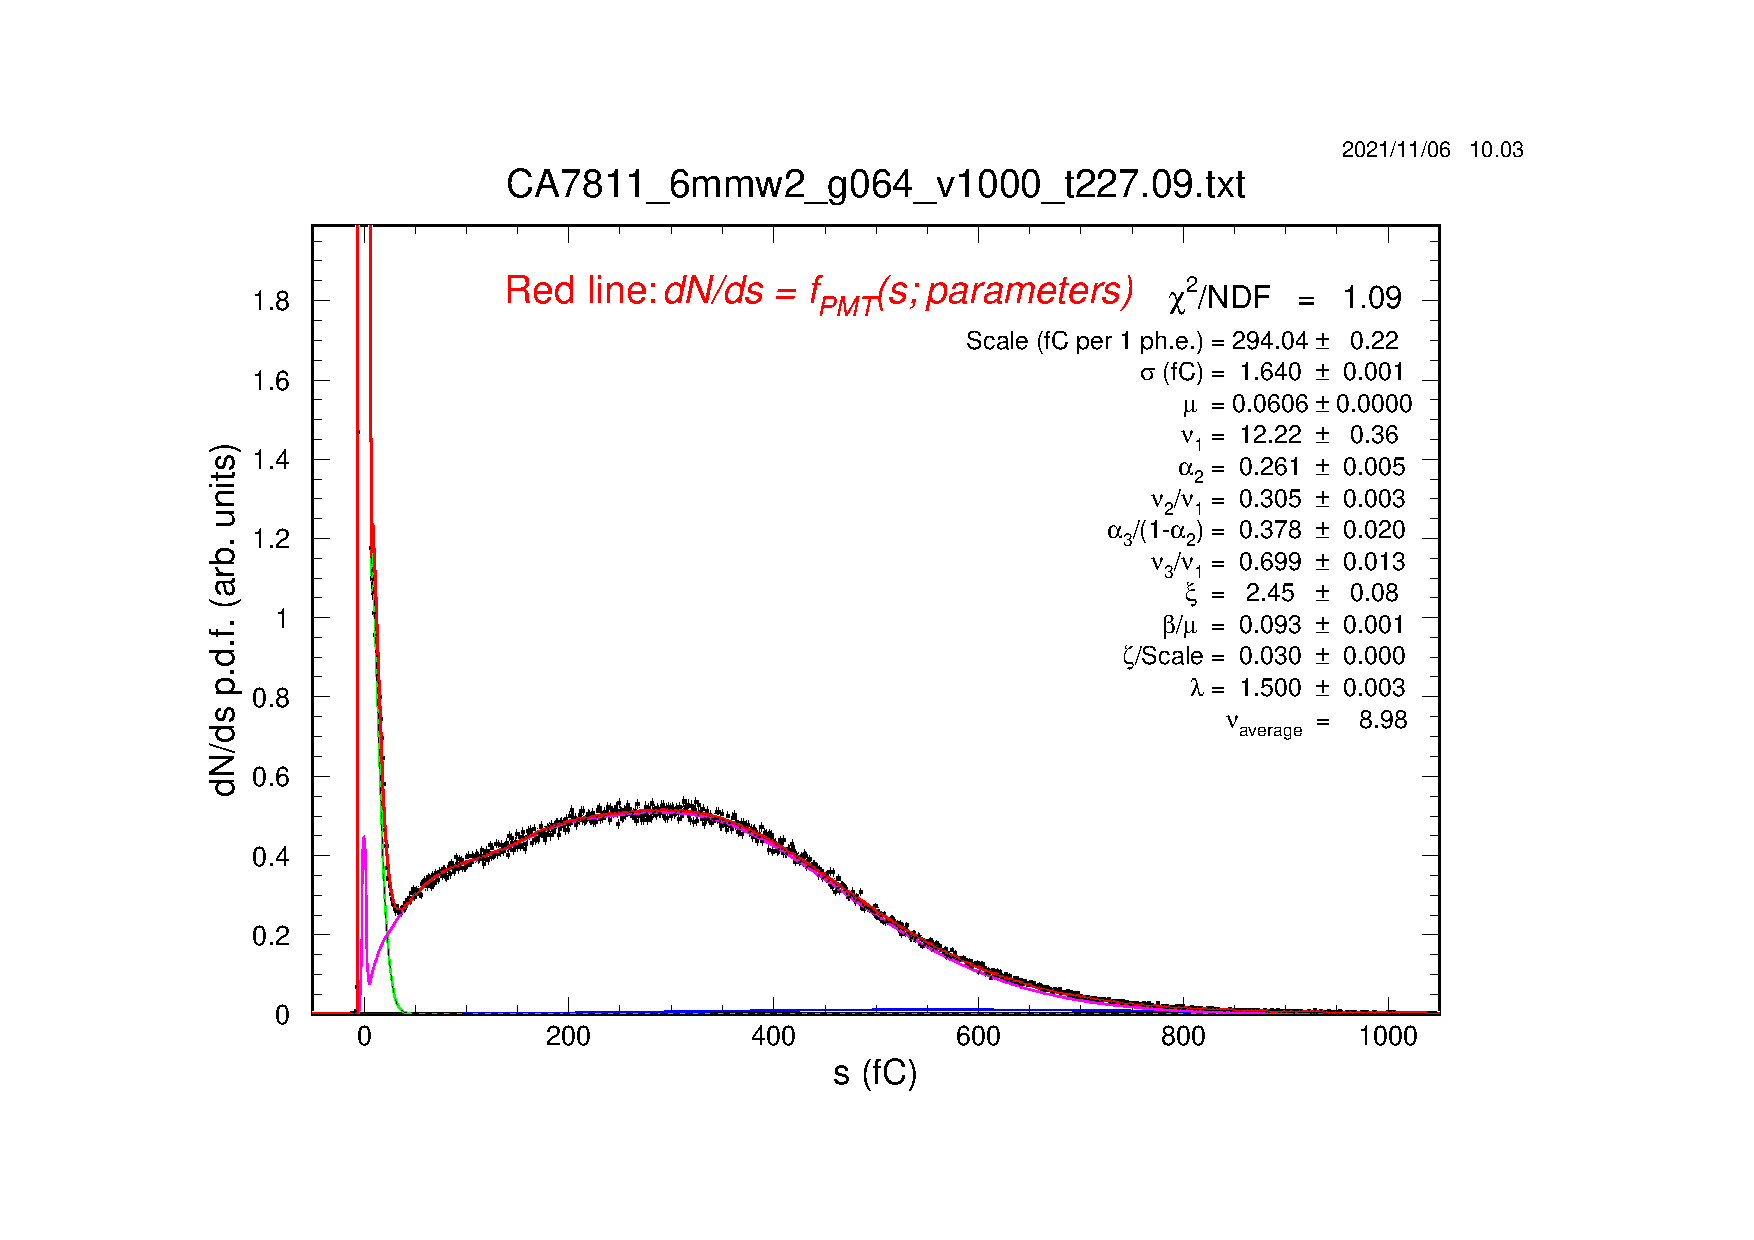
\includegraphics[clip=true,trim=100 75 140 100,width=.49\textwidth,height=.25\textwidth]
                    {figures/CA7811_b.pdf}} \\
  \subfloat[No mask, cross talk removed by software]{%
    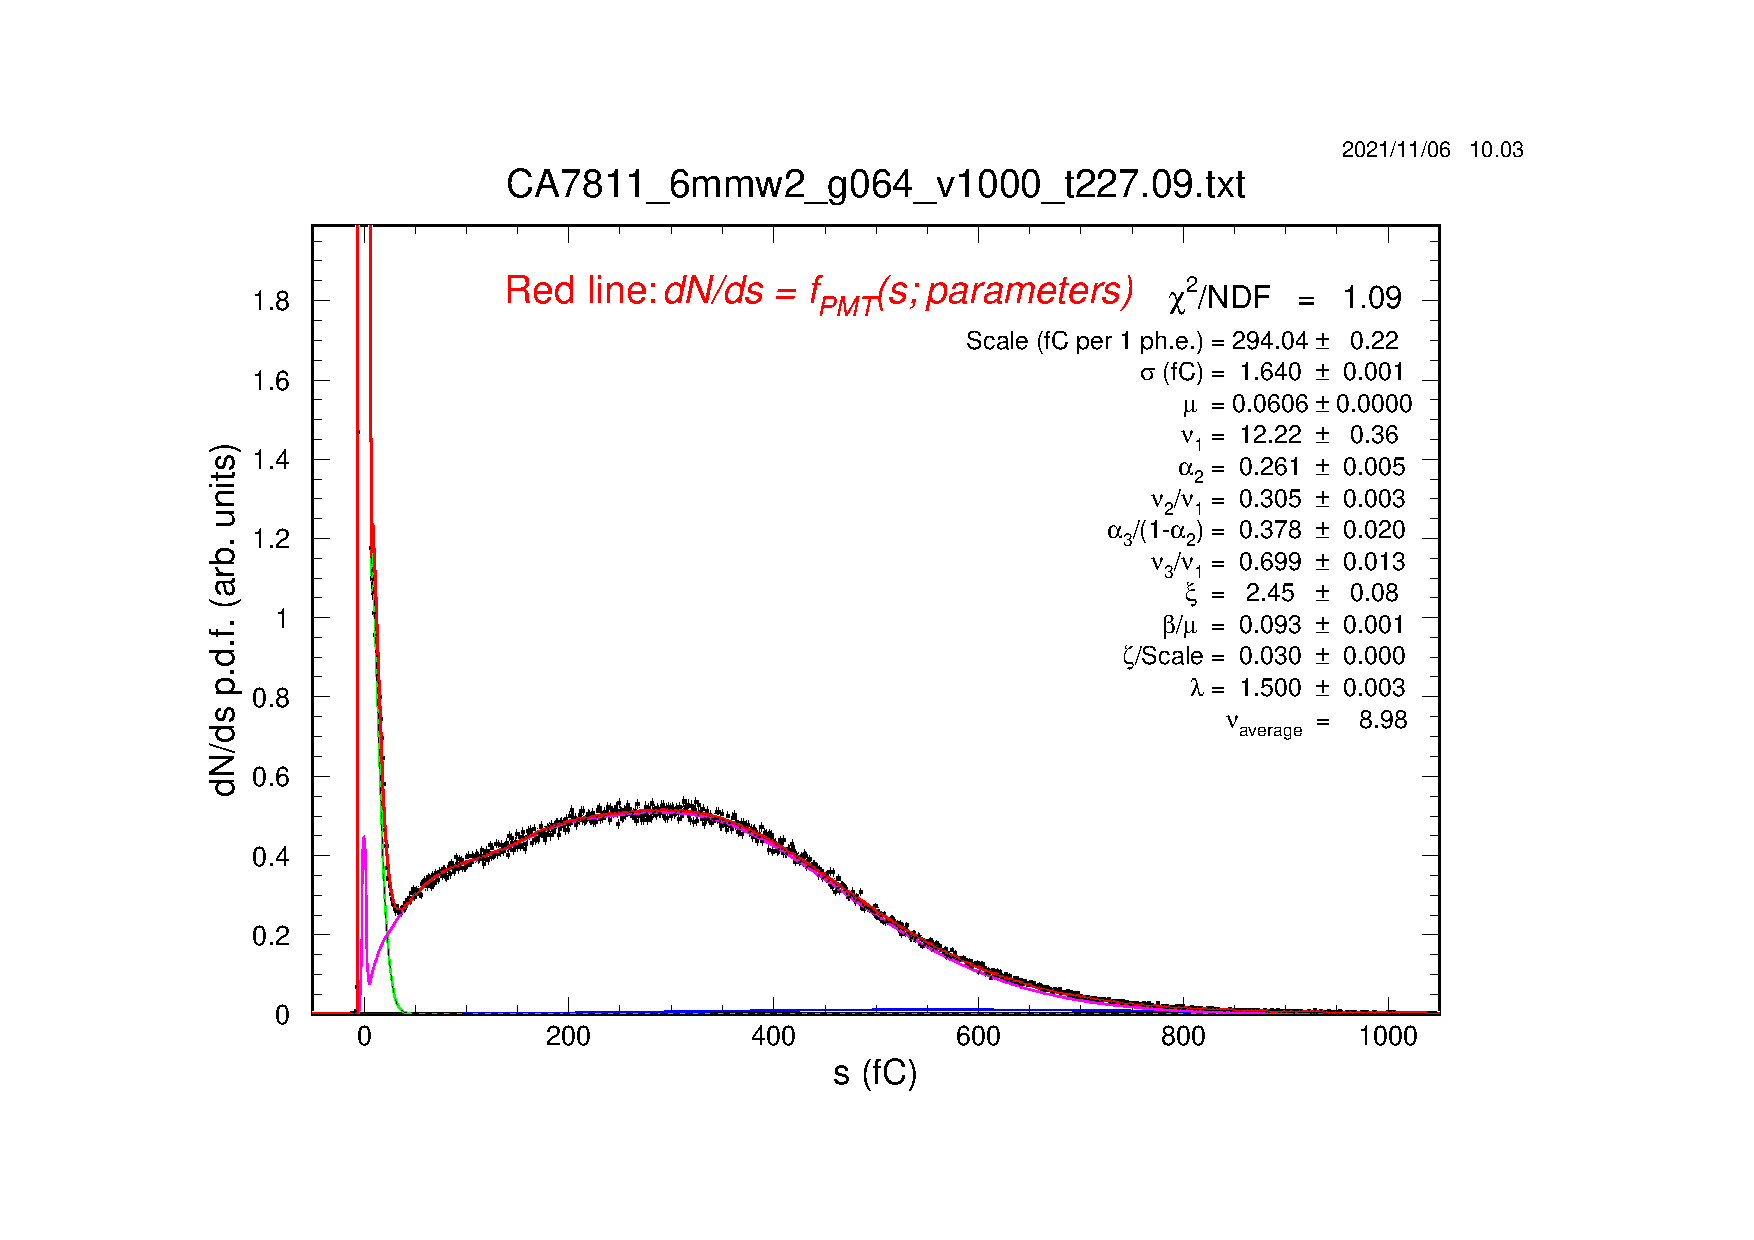
\includegraphics[clip=true,trim=100 75 140 100,width=.49\textwidth,height=.25\textwidth]
                    {figures/CA7811_c.pdf}}
  \subfloat[No mask, cross talk approximated by fit]{%
    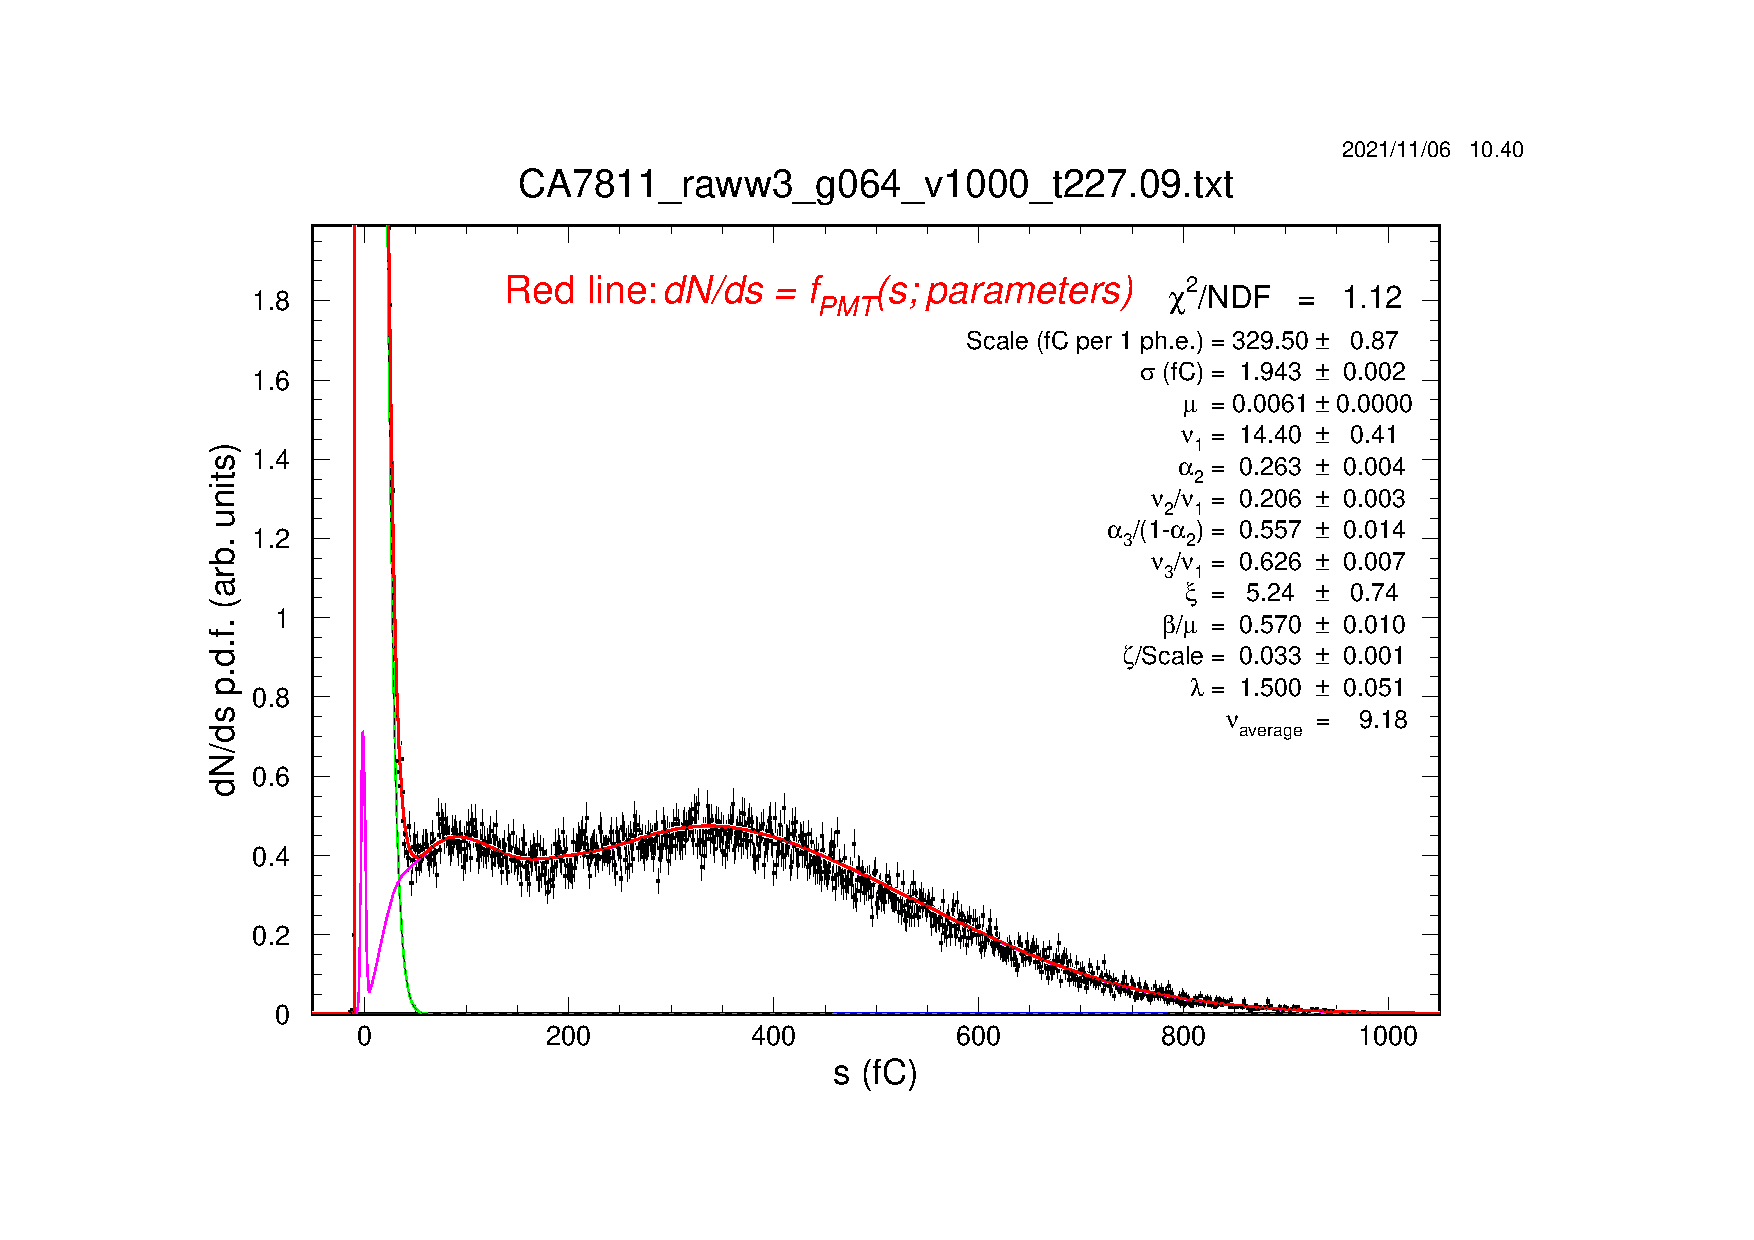
\includegraphics[clip=true,trim=100 75 140 100,width=.49\textwidth,height=.25\textwidth]
                    {figures/CA7811_d.pdf}}
  \caption{Signal amplitude probability distributions for PMT CA7811 (H8500), pixel 9, at HV = 1000 V. a) 3~mm mask. b) 6~mm mask. c) run with full PMT face open with the crosstalk events removed by the correlation analysis. d) run with full PMT face open with the contribution to the spectrum from the crosstalk events approximated and parameterized by the analysis algorithm. The crosstalk effects are too wide to be approximated correctly.
    }
\label{fig:CA7811}
\end{figure*}

\begin{figure*}[hbt] 
\centering 
  \subfloat[3 mm mask]{%
    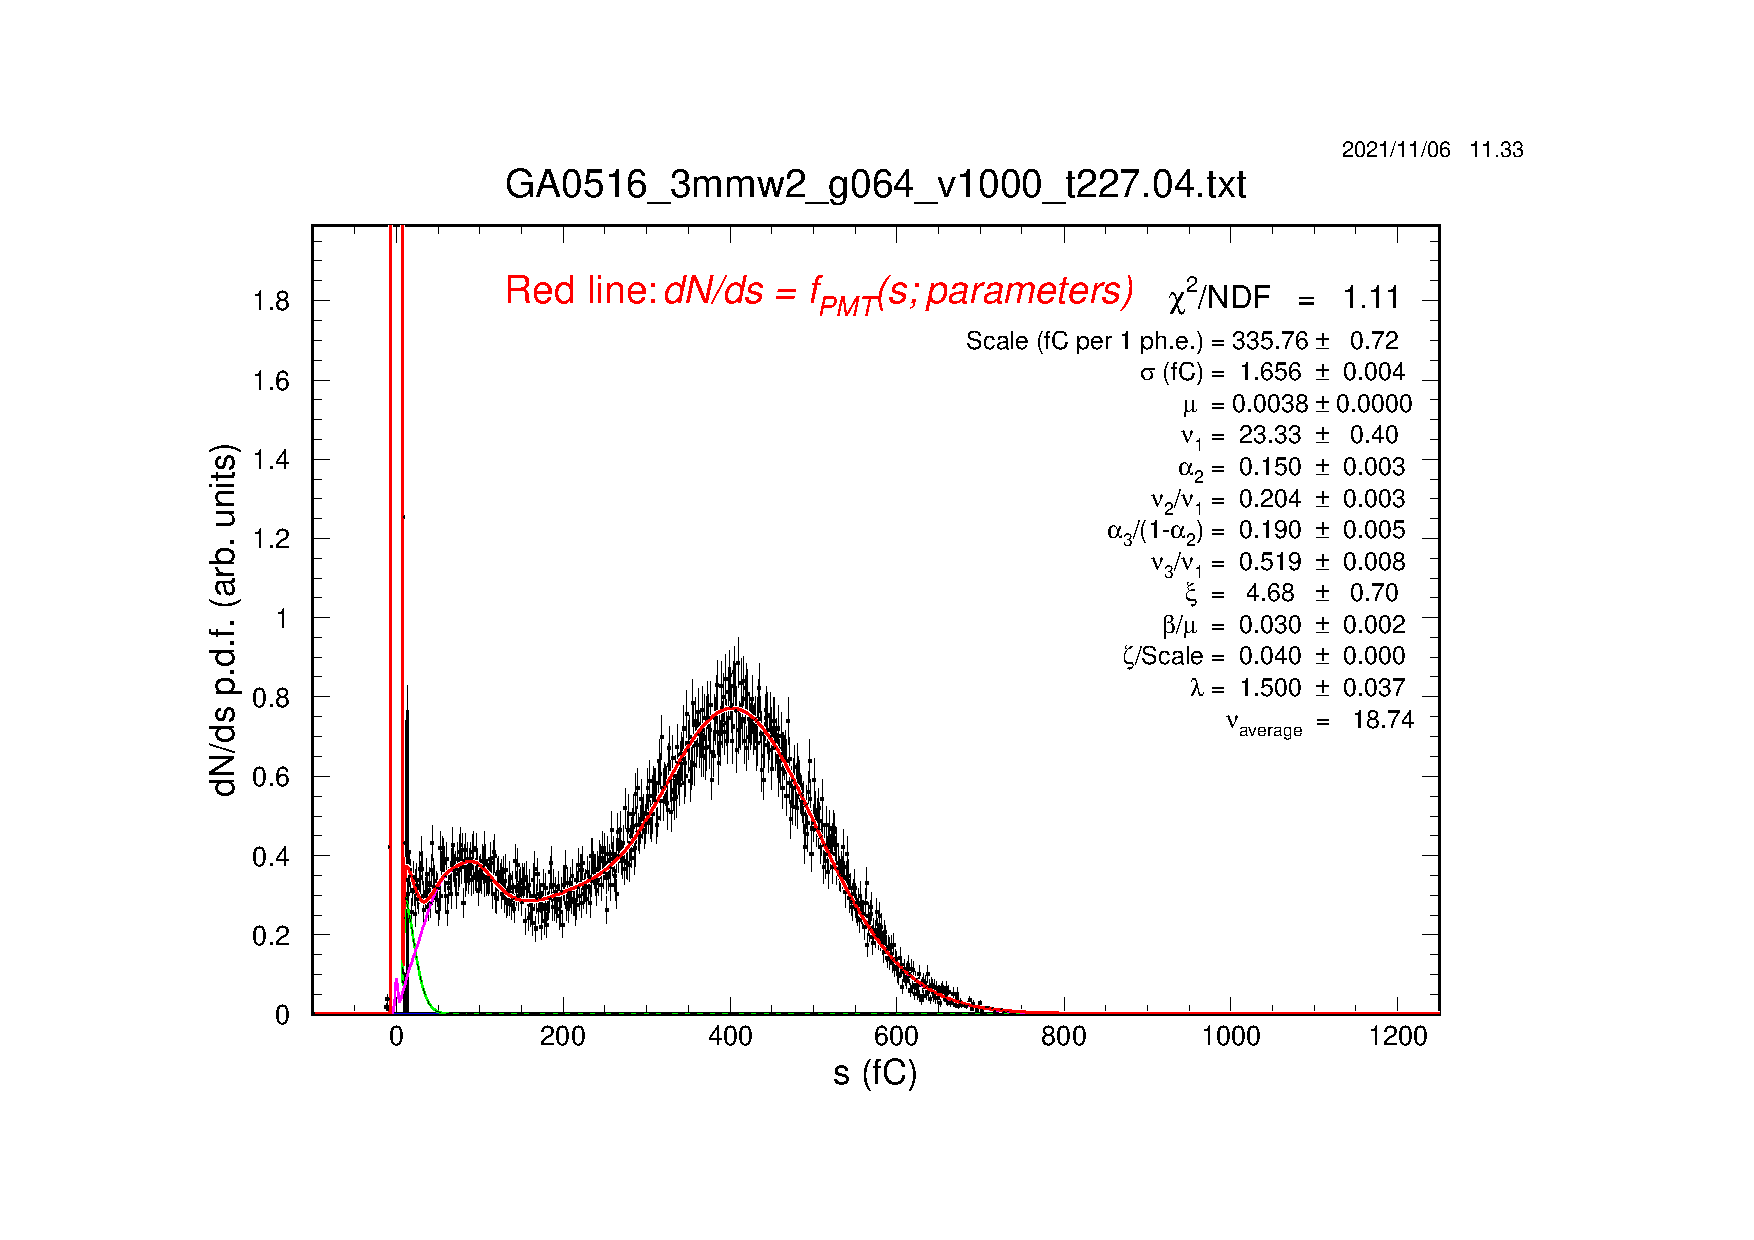
\includegraphics[clip=true,trim=100 75 140 100,width=.49\textwidth,height=.25\textwidth]
                    {figures/GA0516_1a.pdf}}
  \subfloat[6 mm mask]{%
    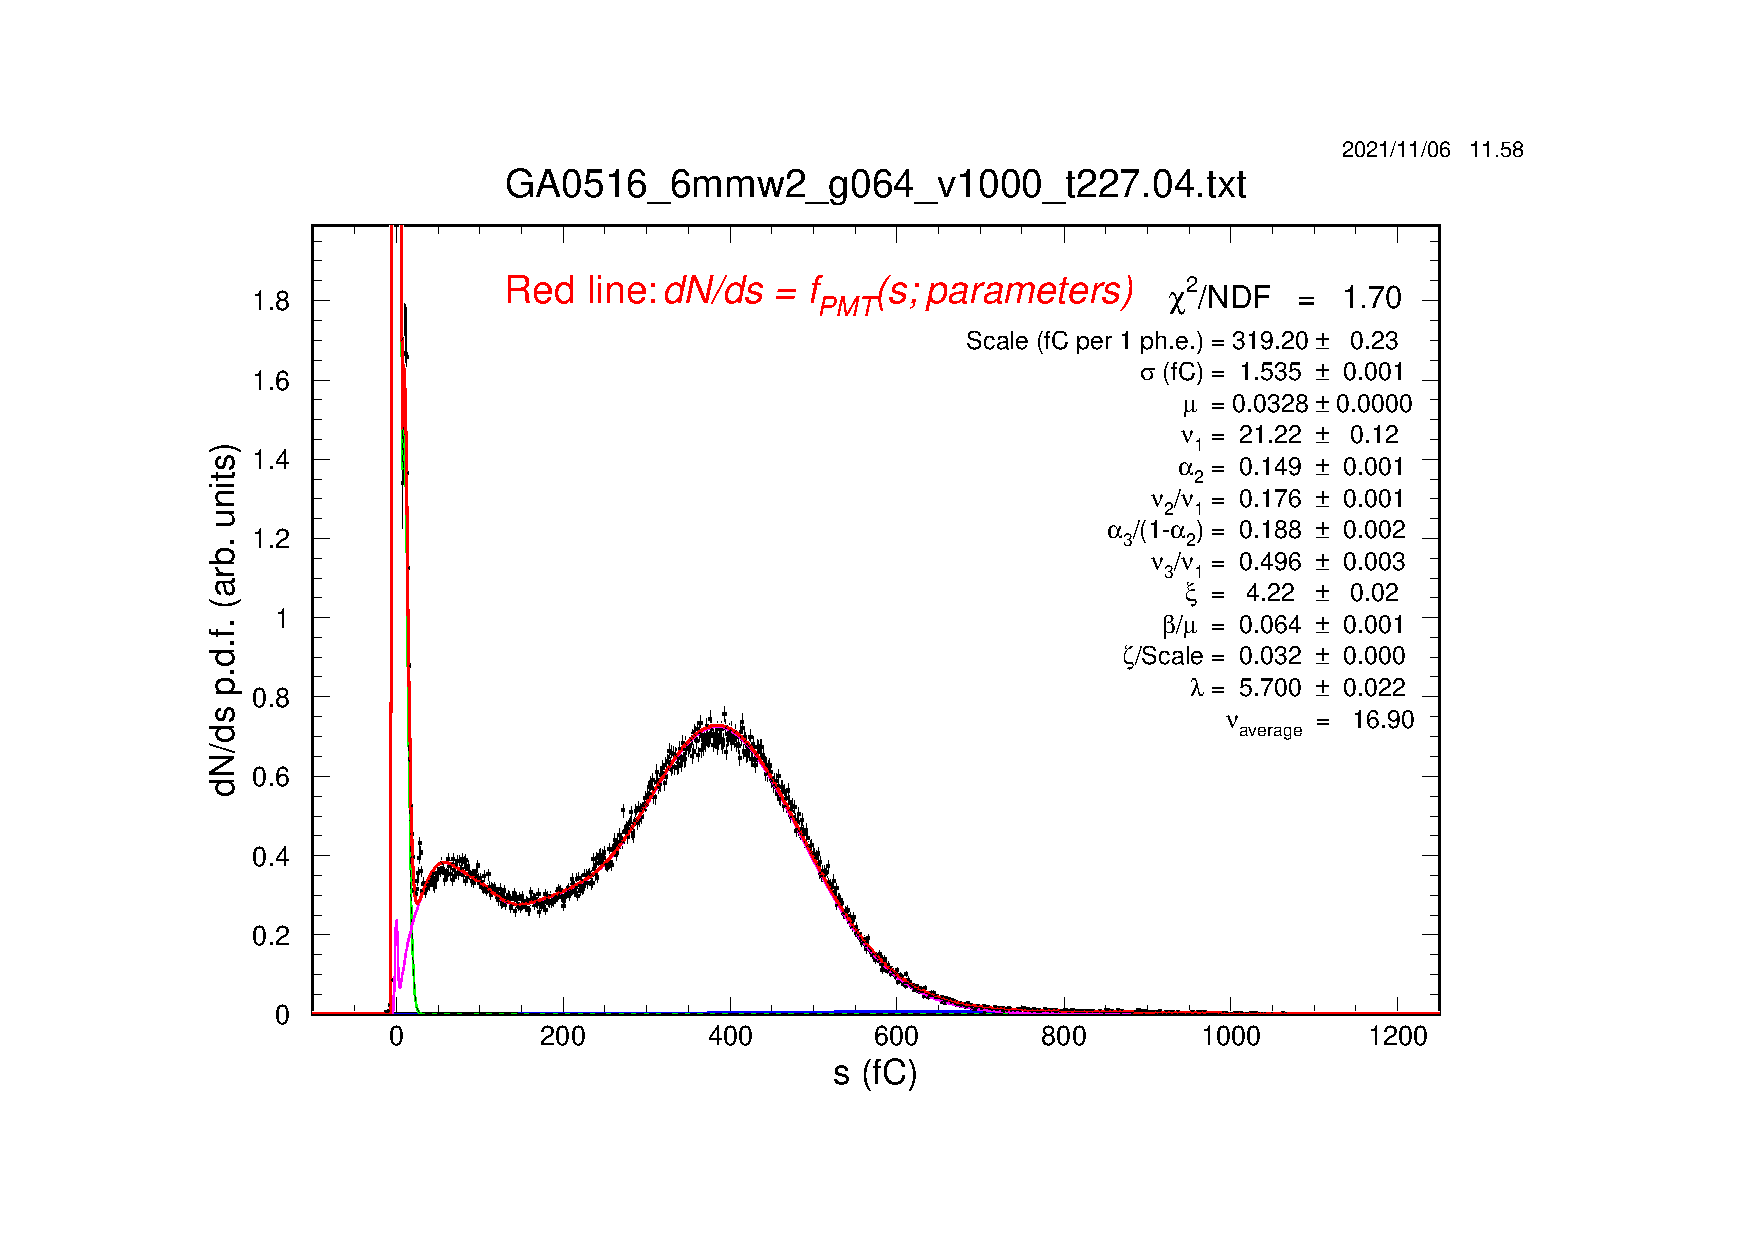
\includegraphics[clip=true,trim=100 75 140 100,width=.49\textwidth,height=.25\textwidth]
                    {figures/GA0516_1b.pdf}} \\
  \subfloat[No mask, cross talk removed by software]{%
    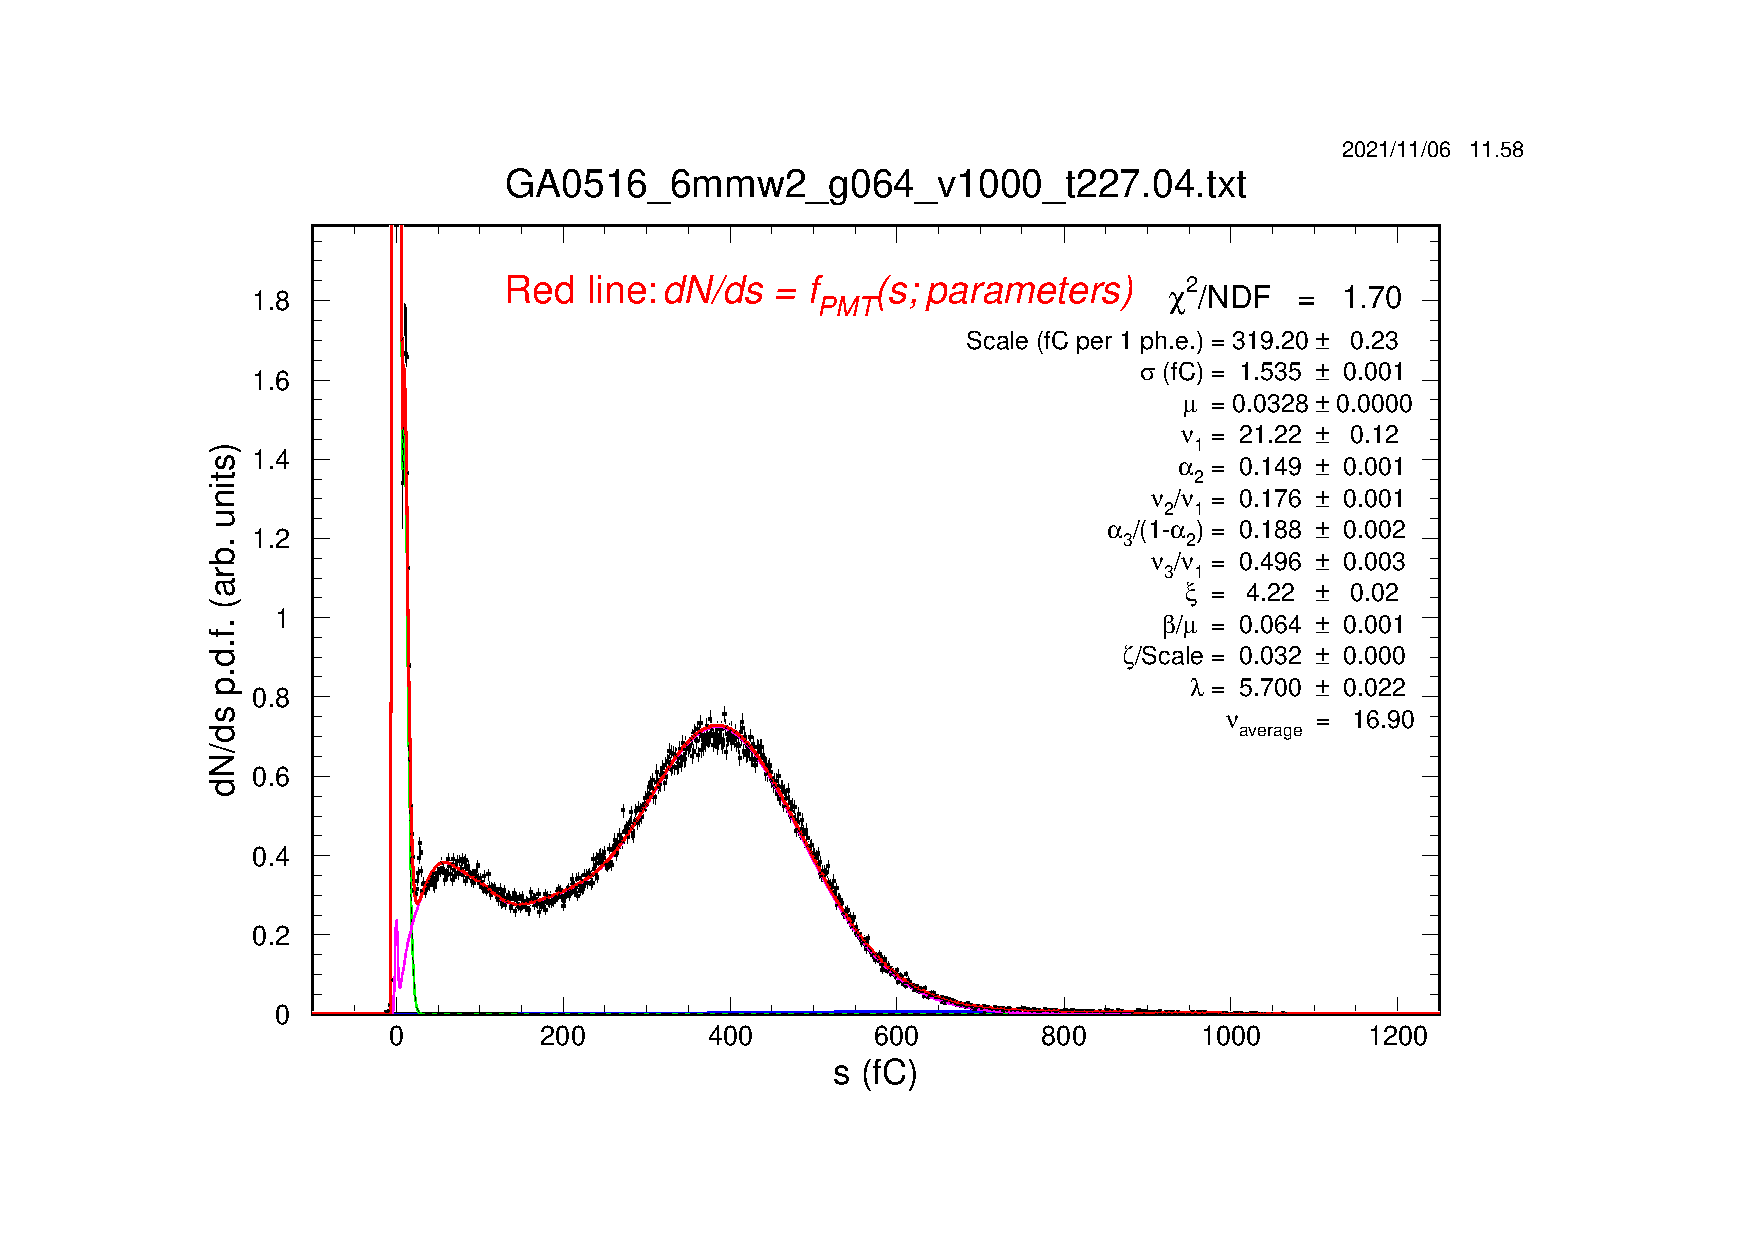
\includegraphics[clip=true,trim=100 75 140 100,width=.49\textwidth,height=.25\textwidth]
                    {figures/GA0516_1c.pdf}}
  \subfloat[No mask, cross talk approximated by fit]{%
    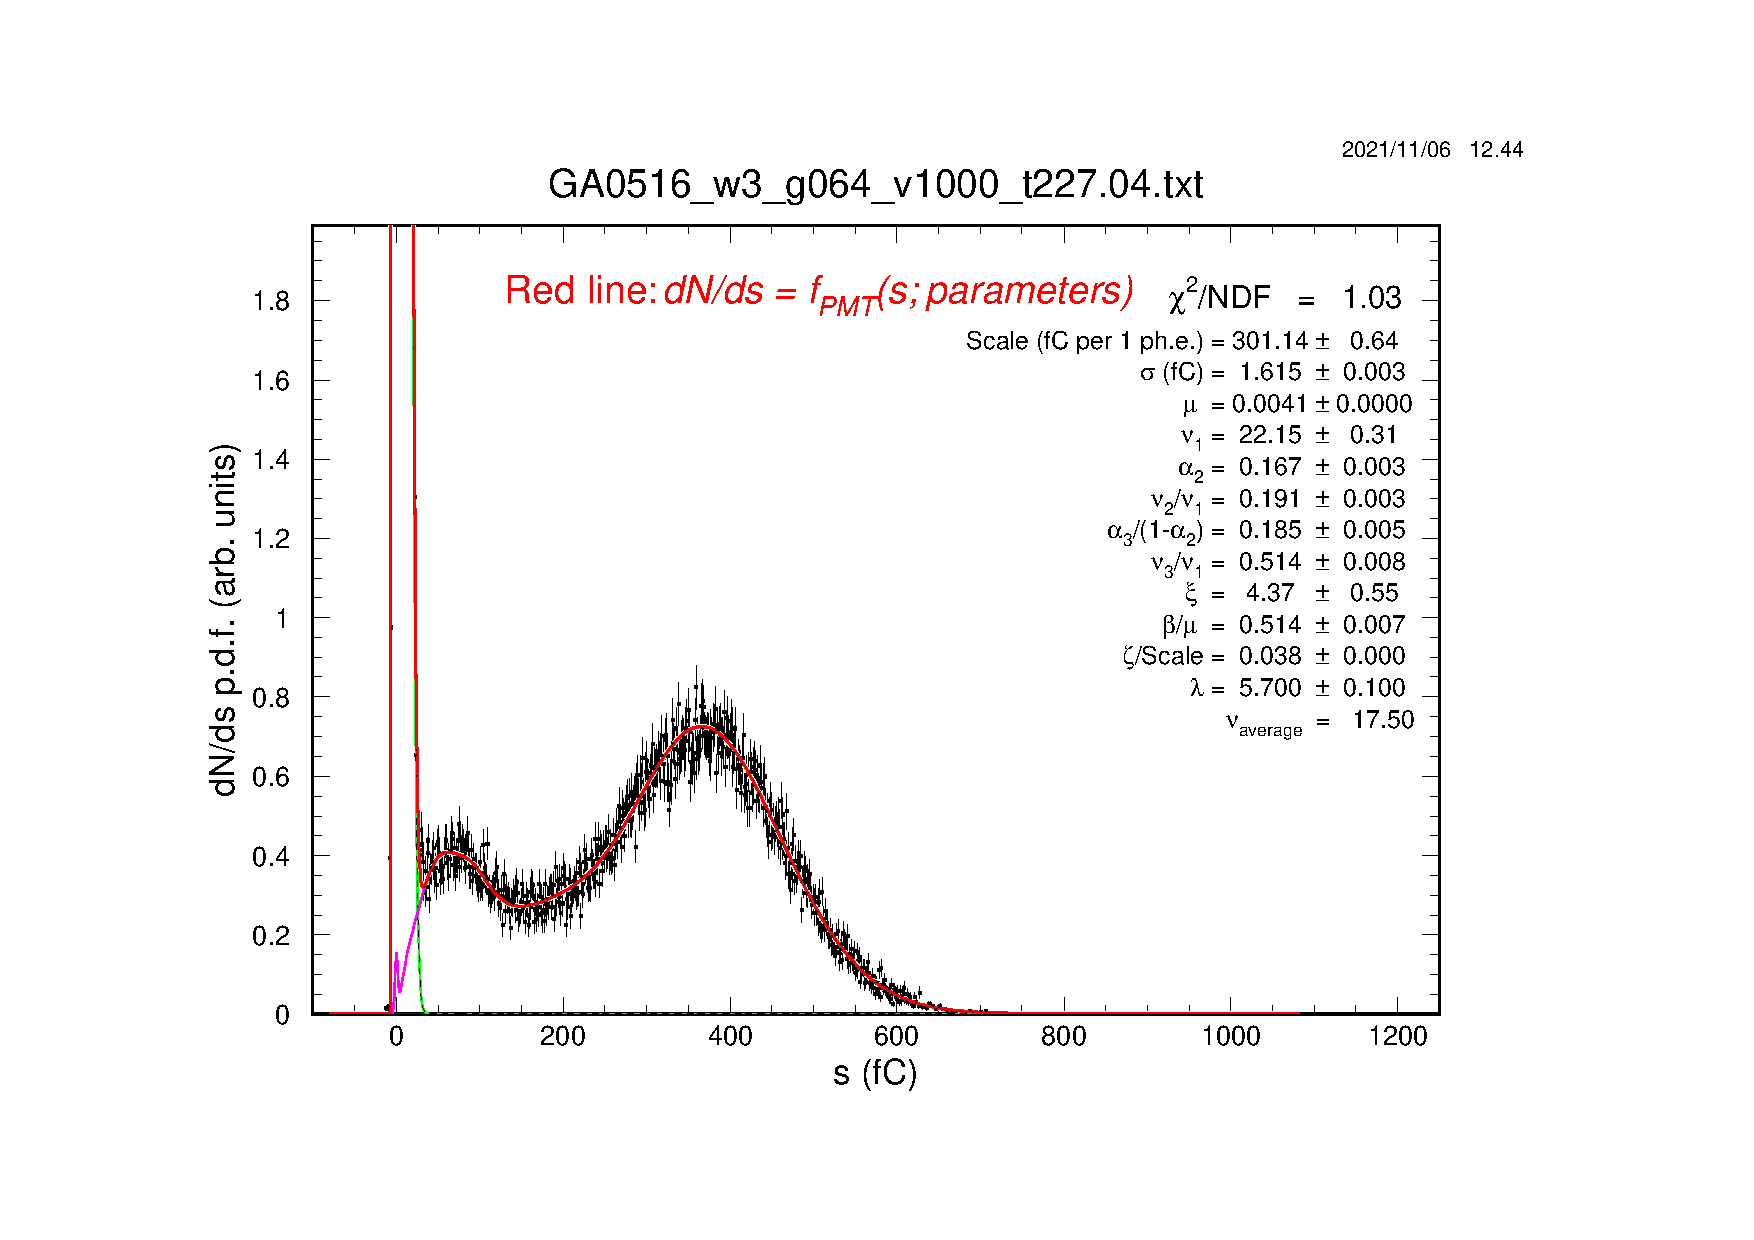
\includegraphics[clip=true,trim=100 75 140 100,width=.49\textwidth,height=.25\textwidth]
                    {figures/GA0516_1d.pdf}}
  \caption{Signal amplitude probability distributions for PMT GA0516 (H12700), pixel 4, at HV = 1000 V. a) 3~mm mask. b) 6~mm mask. c) run with full PMT face open with the crosstalk events removed by the correlation analysis. d) run with full PMT face open with the contribution to the spectrum from the crosstalk events approximated and parameterized by the analysis algorithm.
    }
\label{fig:GA0516_1}
\end{figure*}
\begin{figure*}[h!bt] 
\centering 
  \subfloat[3 mm mask]{%
    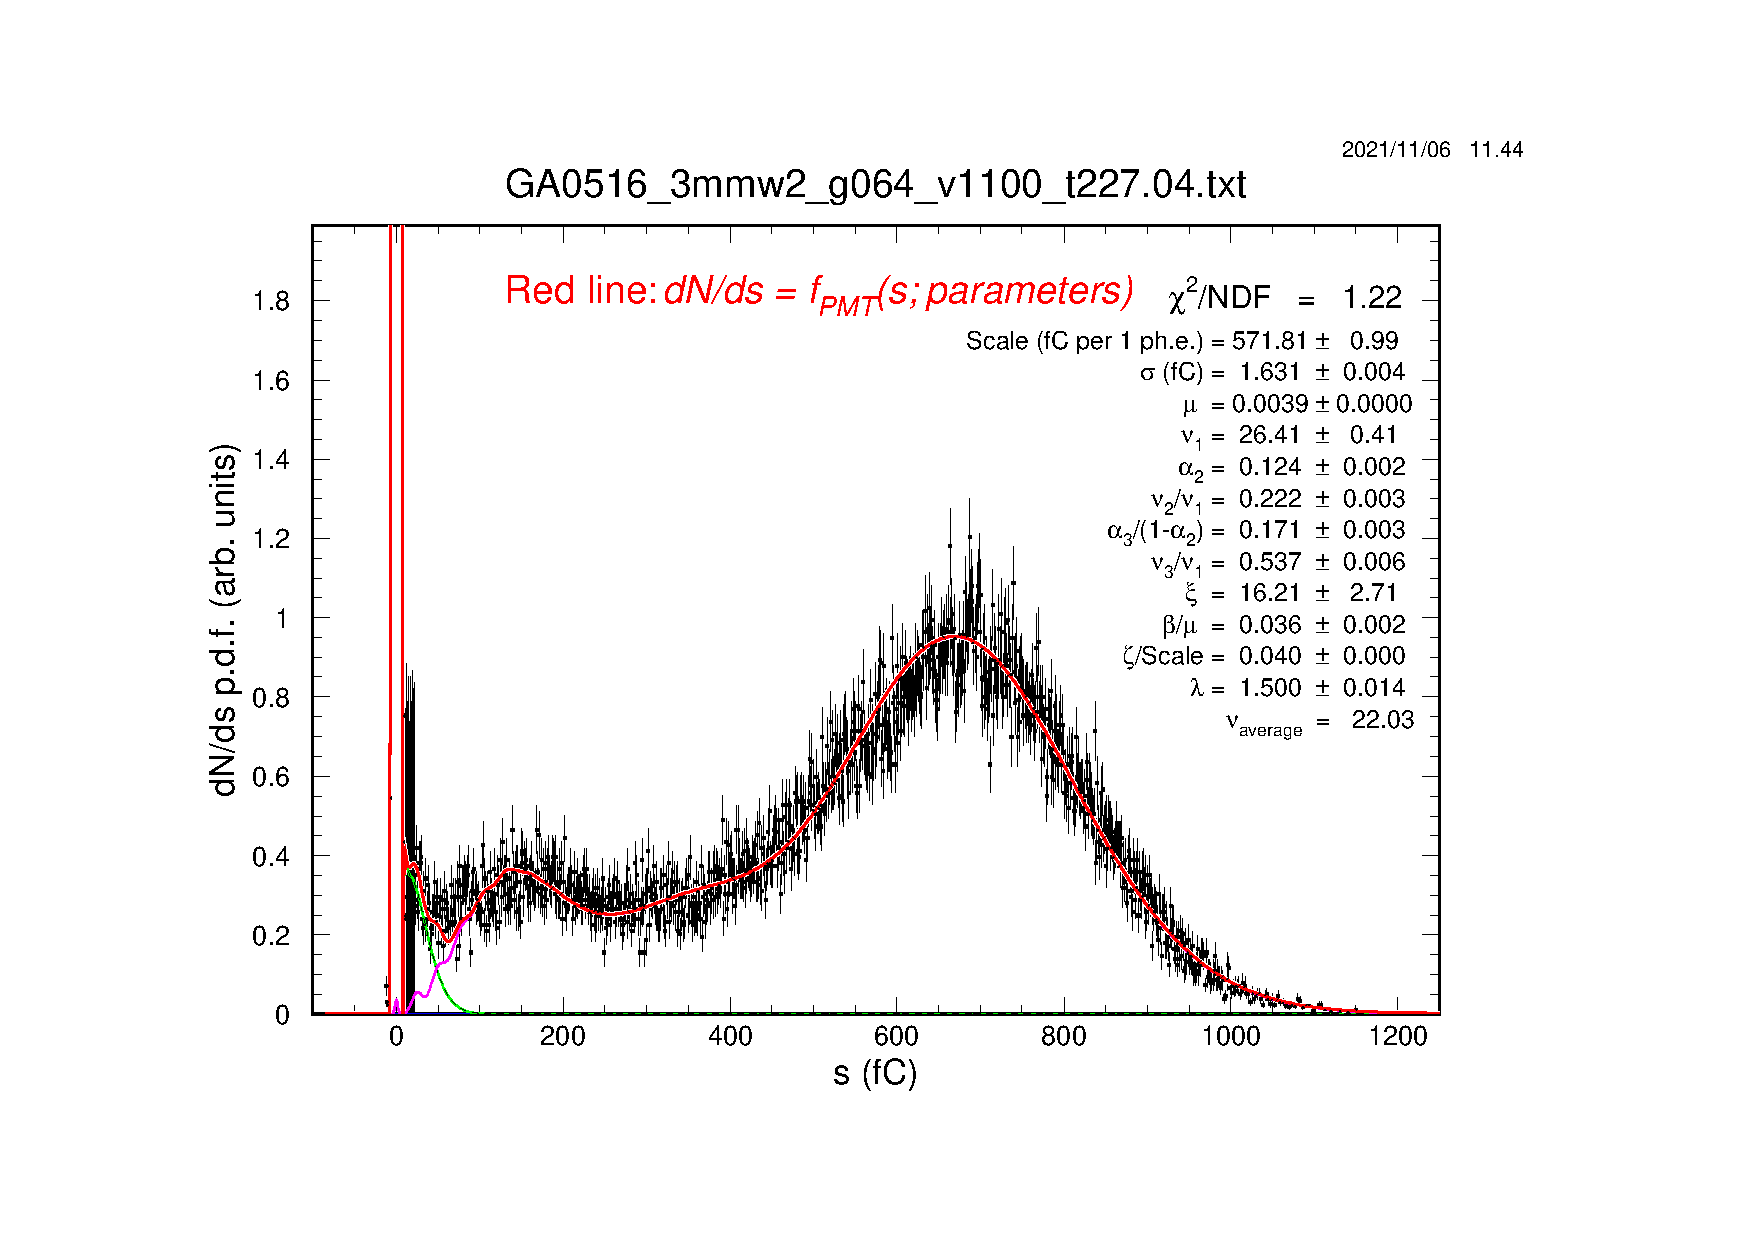
\includegraphics[clip=true,trim=100 75 140 100,width=.49\textwidth,height=.25\textwidth]
                    {figures/GA0516_2a.pdf}}
  \subfloat[6 mm mask]{%
    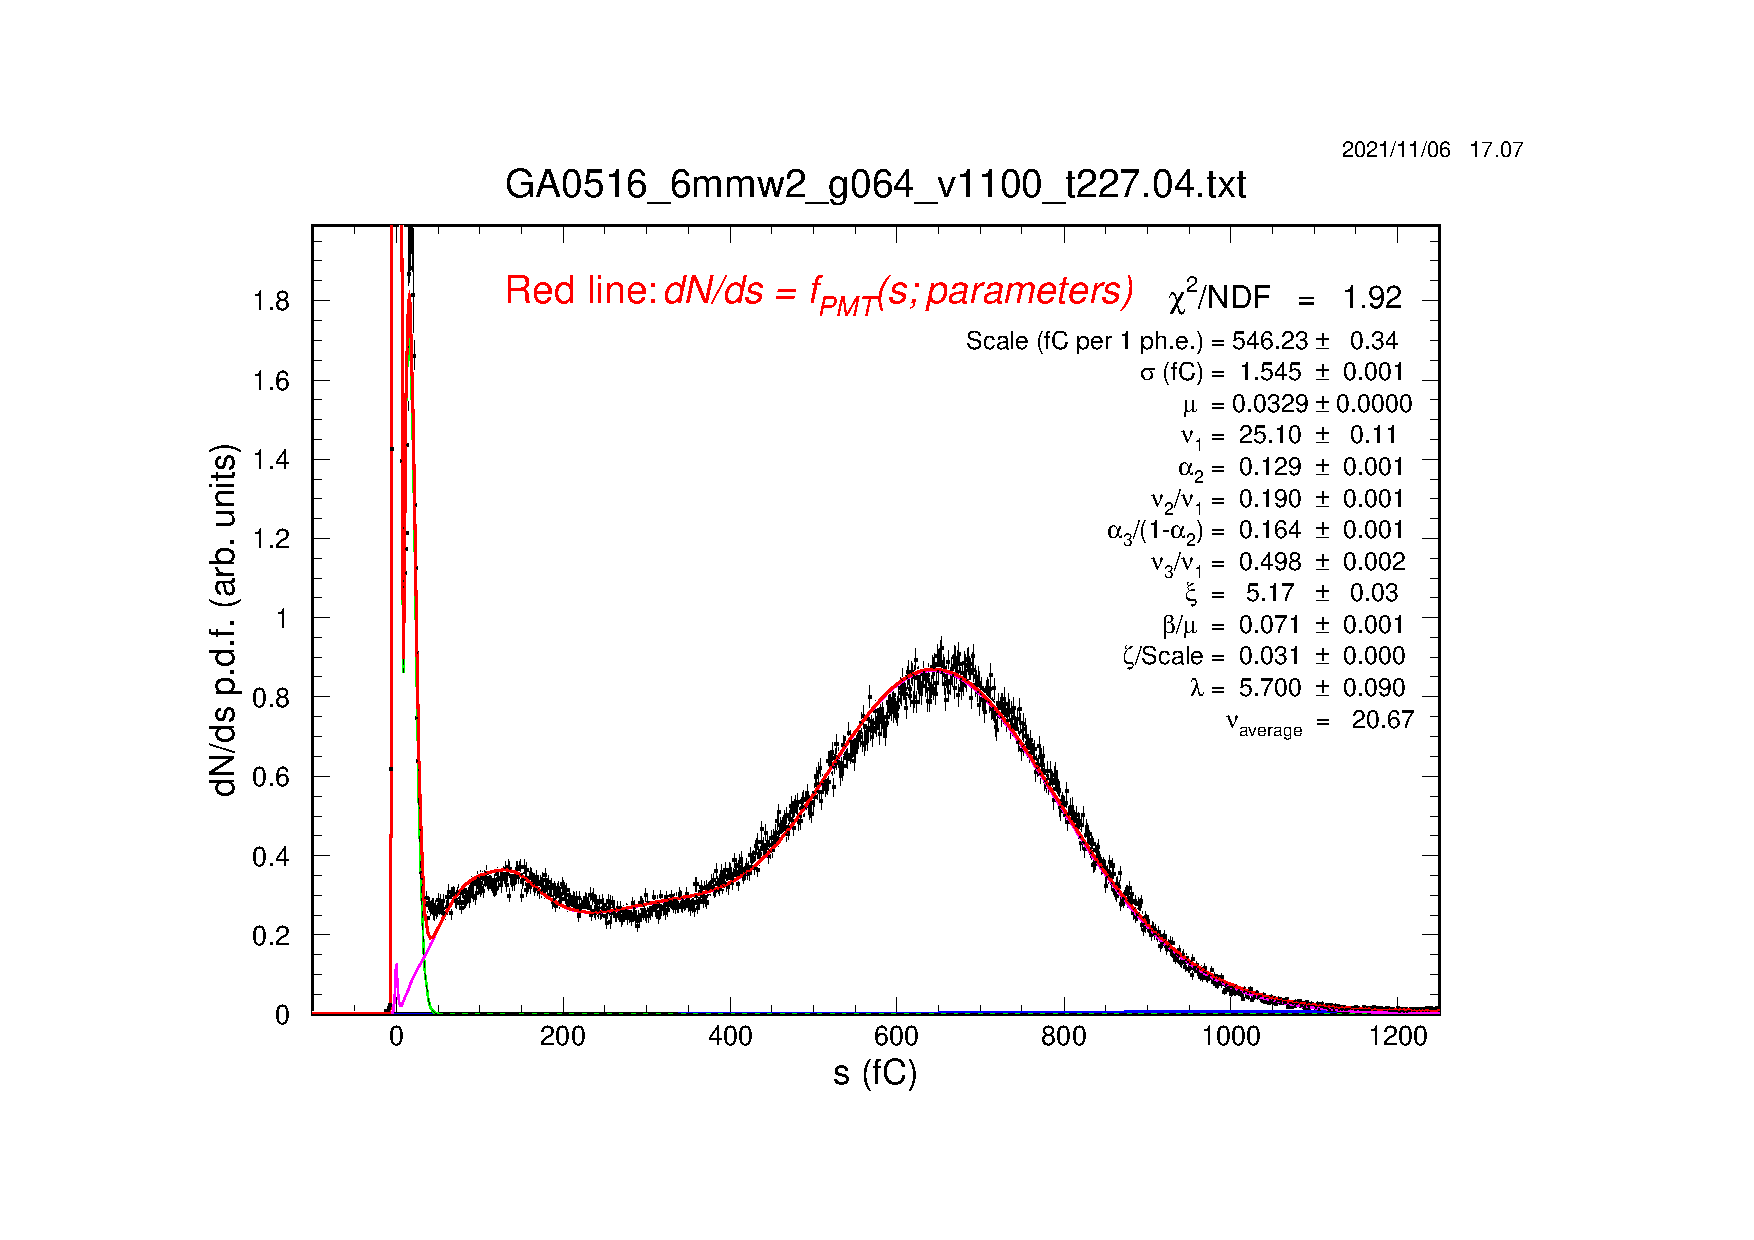
\includegraphics[clip=true,trim=100 75 140 100,width=.49\textwidth,height=.25\textwidth]
                    {figures/GA0516_2b.pdf}} \\
  \subfloat[No mask, cross talk removed by software]{%
    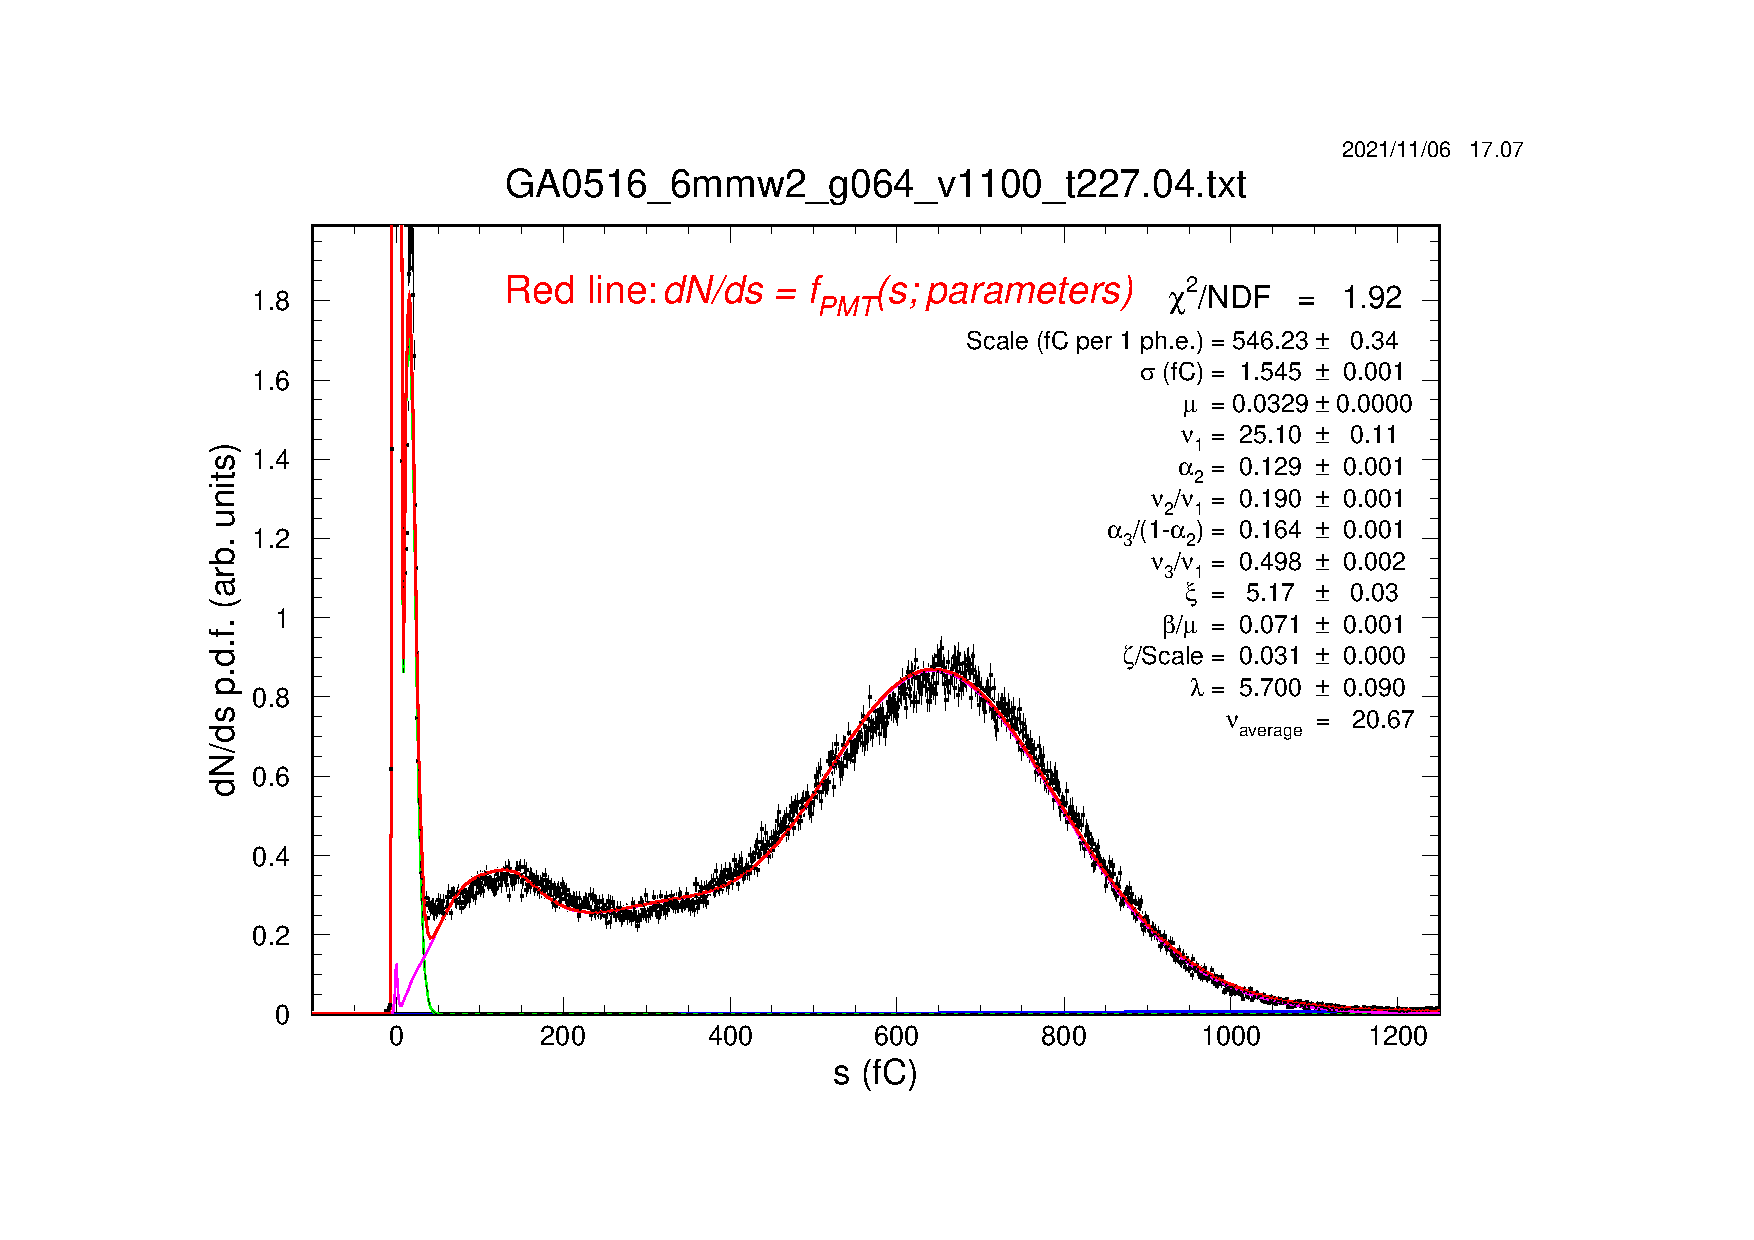
\includegraphics[clip=true,trim=100 75 140 100,width=.49\textwidth,height=.25\textwidth]
                    {figures/GA0516_2c.pdf}}
  \subfloat[No mask, cross talk approximated by fit]{%
    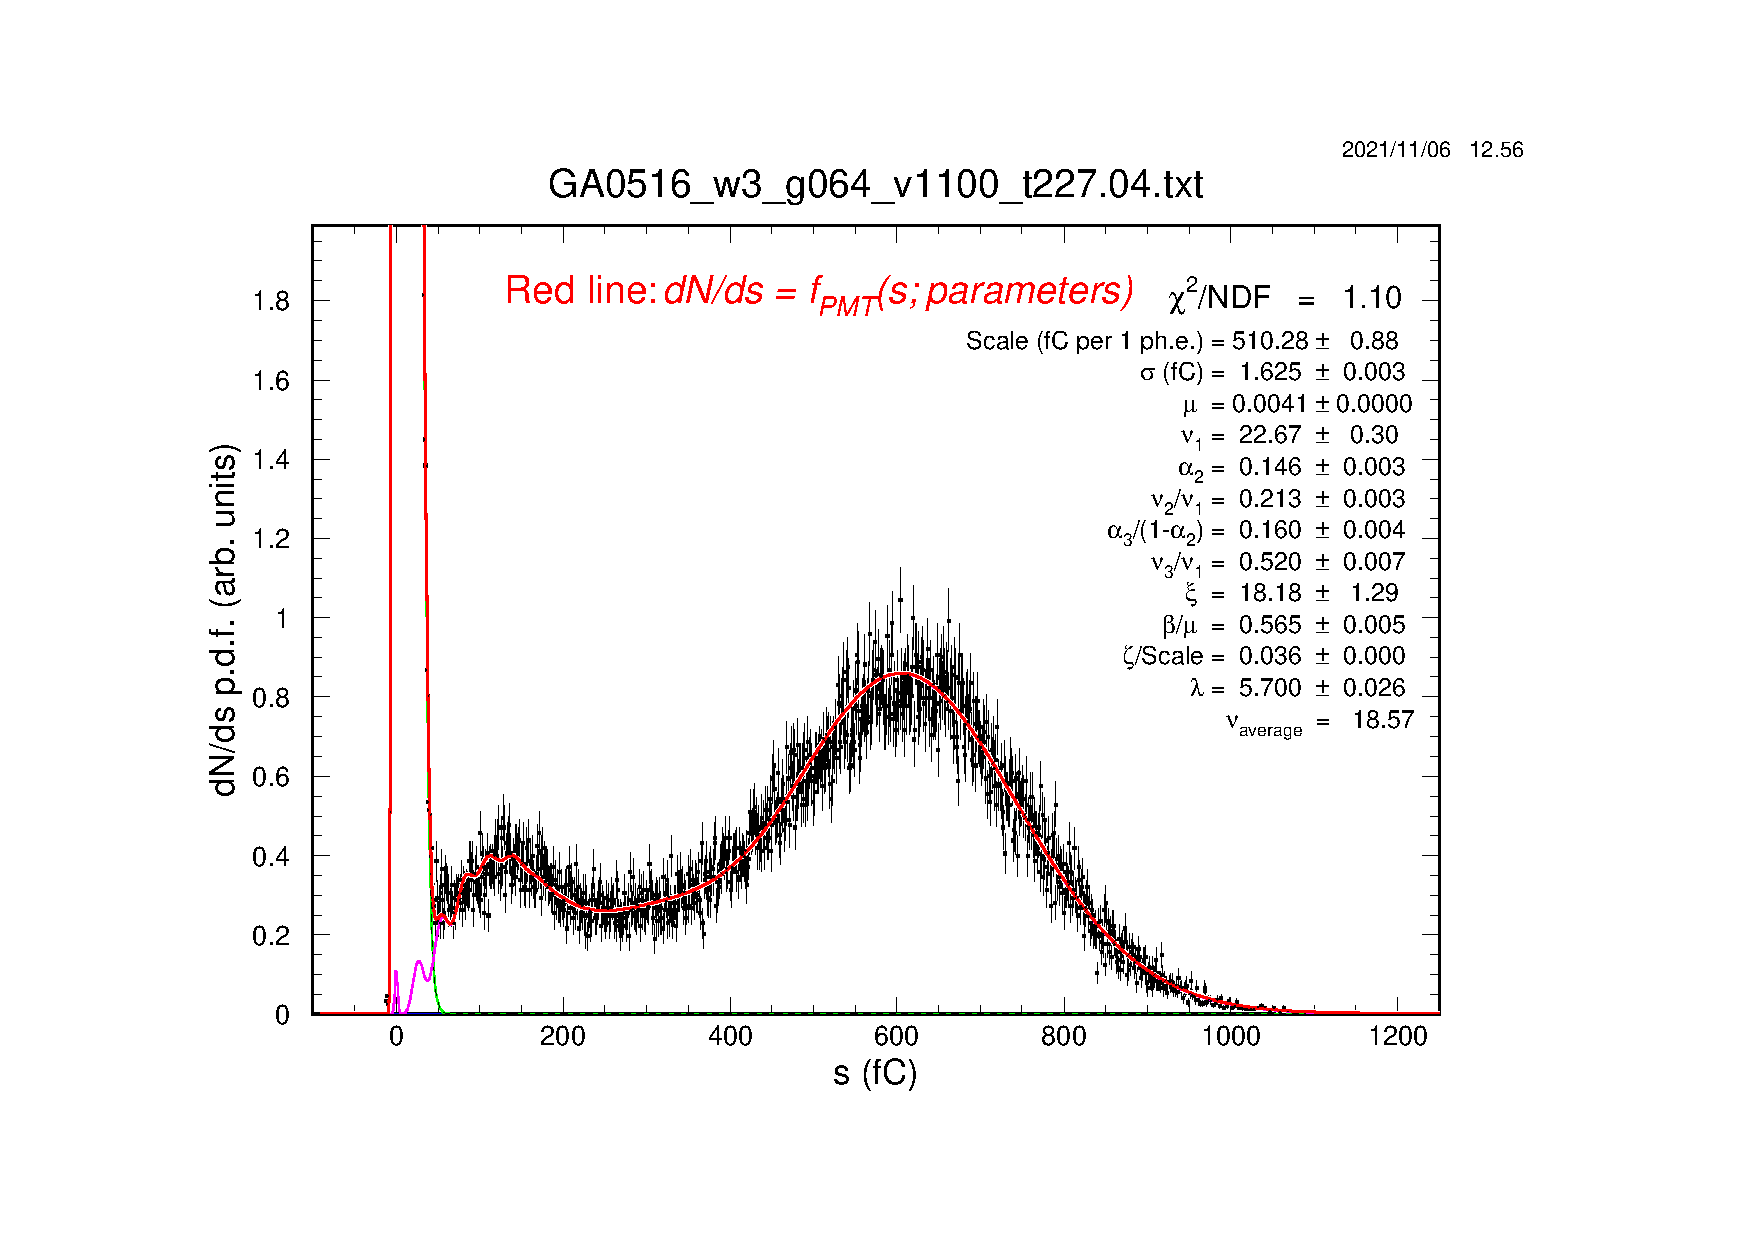
\includegraphics[clip=true,trim=100 75 140 100,width=.49\textwidth,height=.25\textwidth]
                    {figures/GA0516_2d.pdf}}
  \caption{Same as Fig.~\ref{fig:GA0516_1}, but with all the data taken at HV = 1100~V. 
    }
\label{fig:GA0516_2}
\end{figure*}
\begin{figure*}[h!bt] 
\centering 
  \subfloat[6 mm mask, at HV = 1000 V]{%
    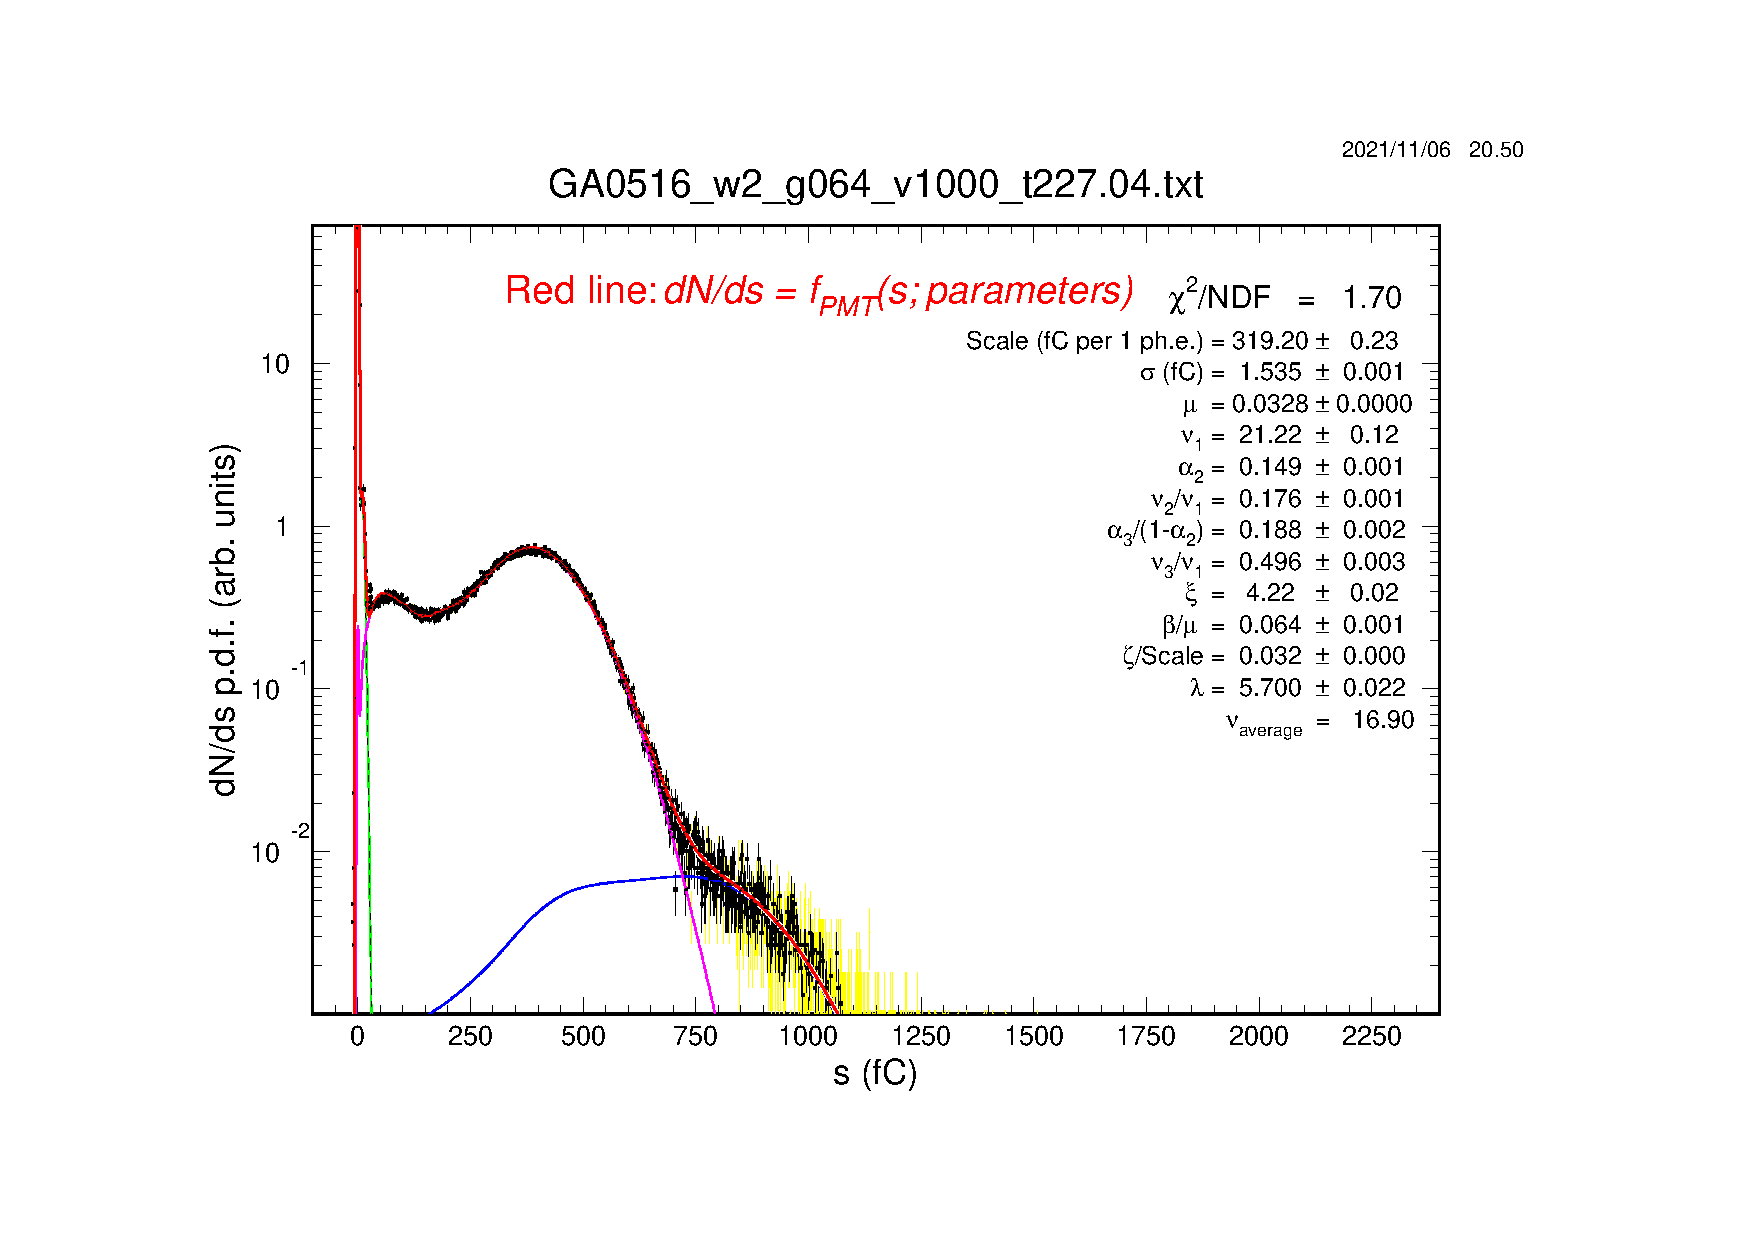
\includegraphics[clip=true,trim=100 75 140 100,width=.49\textwidth,height=.25\textwidth]
                    {figures/GA0516_3a.pdf}}
  \subfloat[6 mm mask, at HV = 1100 V]{%
    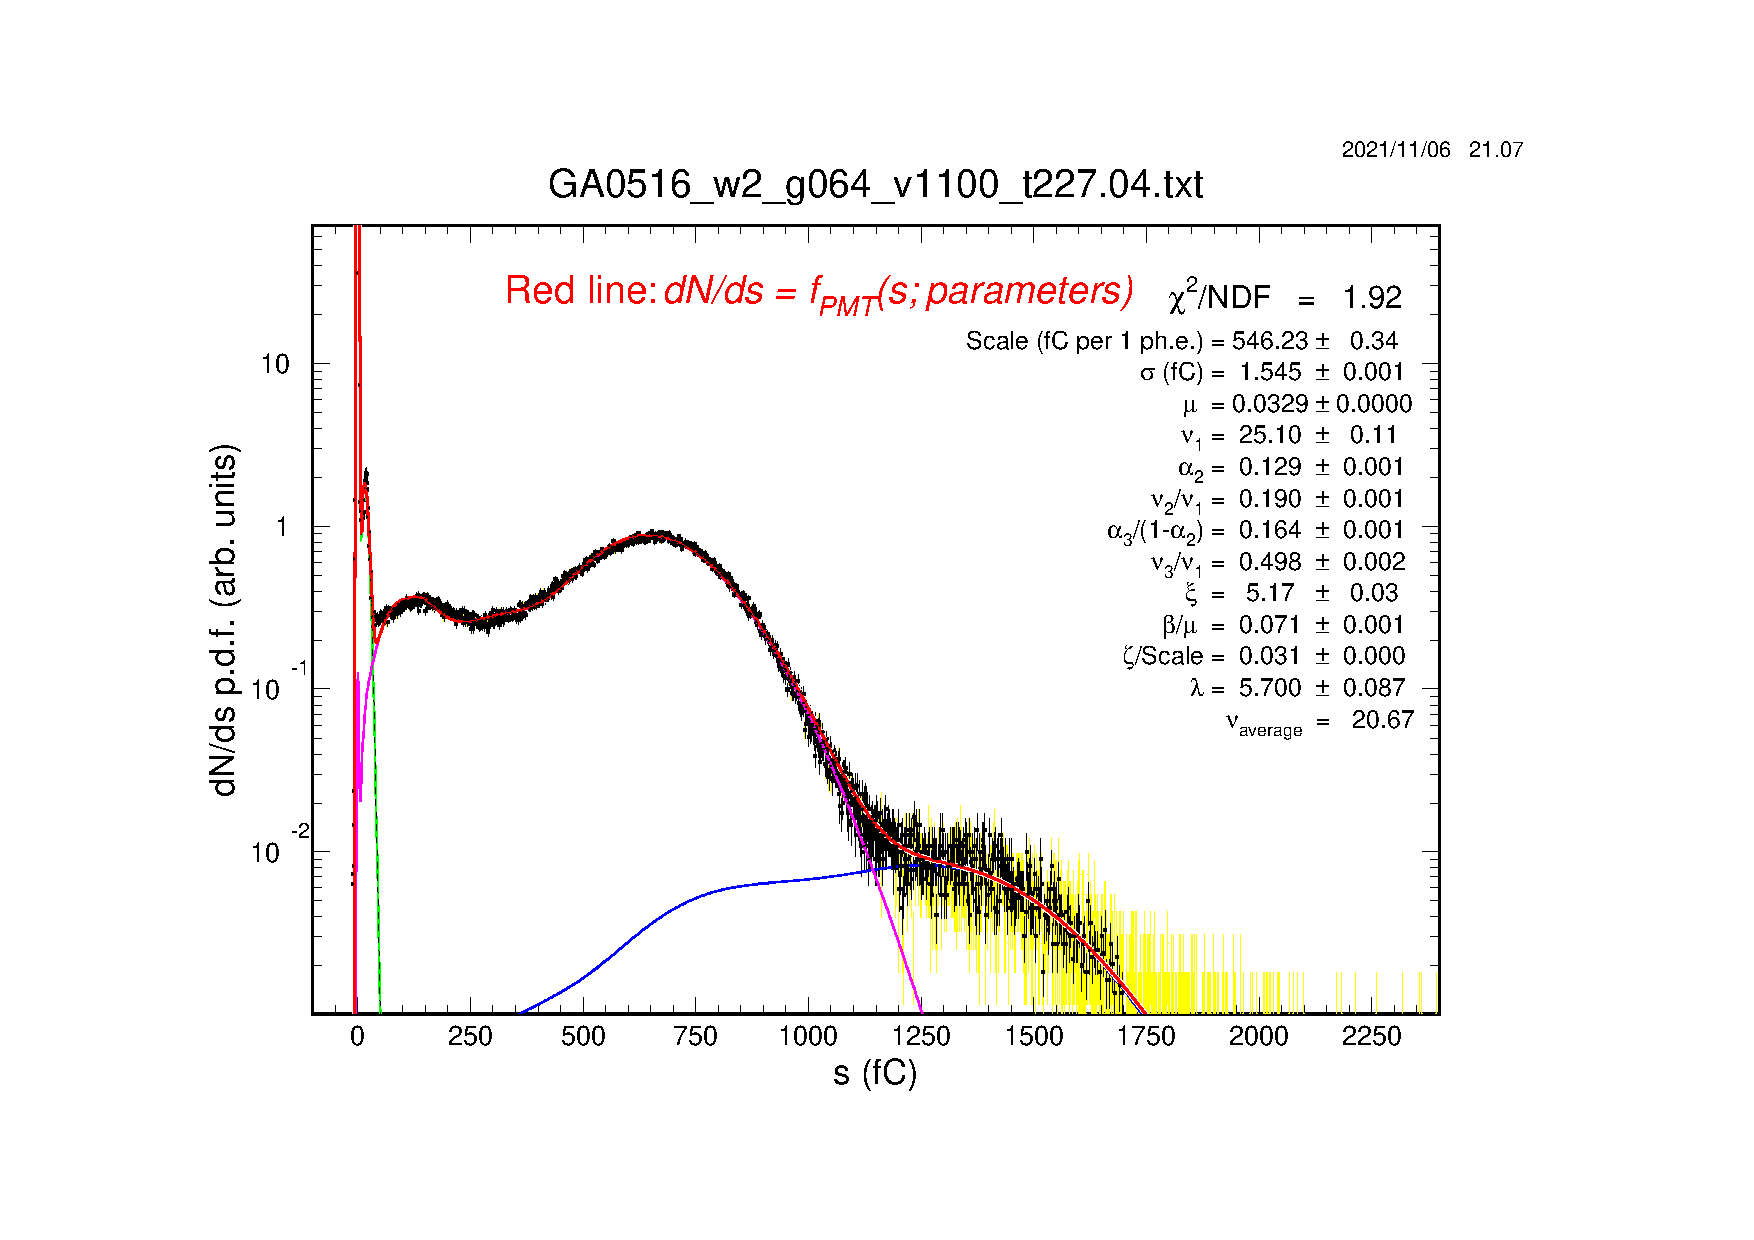
\includegraphics[clip=true,trim=100 75 140 100,width=.49\textwidth,height=.25\textwidth]
                    {figures/GA0516_3b.pdf}} \\
  \subfloat[No mask, at HV = 1000 V]{%
    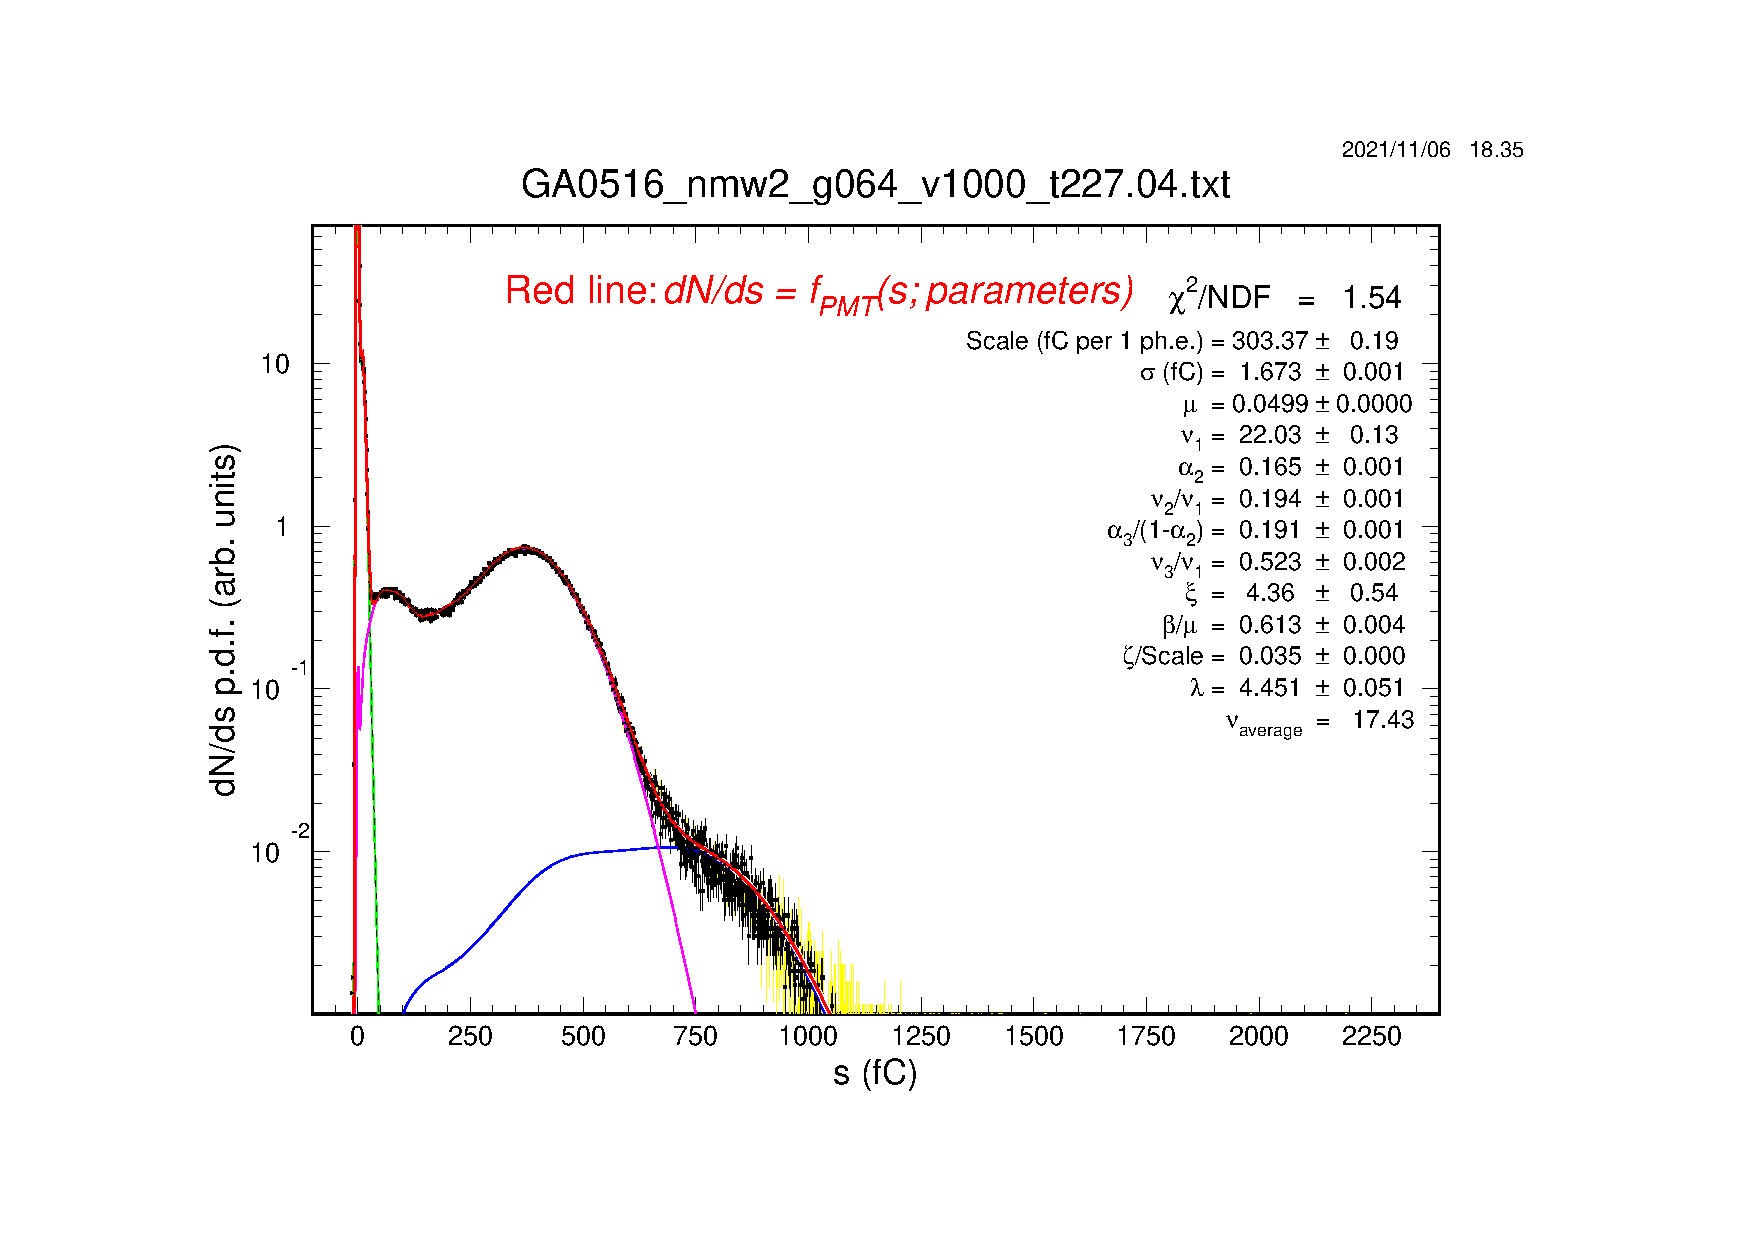
\includegraphics[clip=true,trim=100 75 140 100,width=.49\textwidth,height=.25\textwidth]
                    {figures/GA0516_3c.pdf}}
  \subfloat[No mask, at HV = 1100 V]{%
    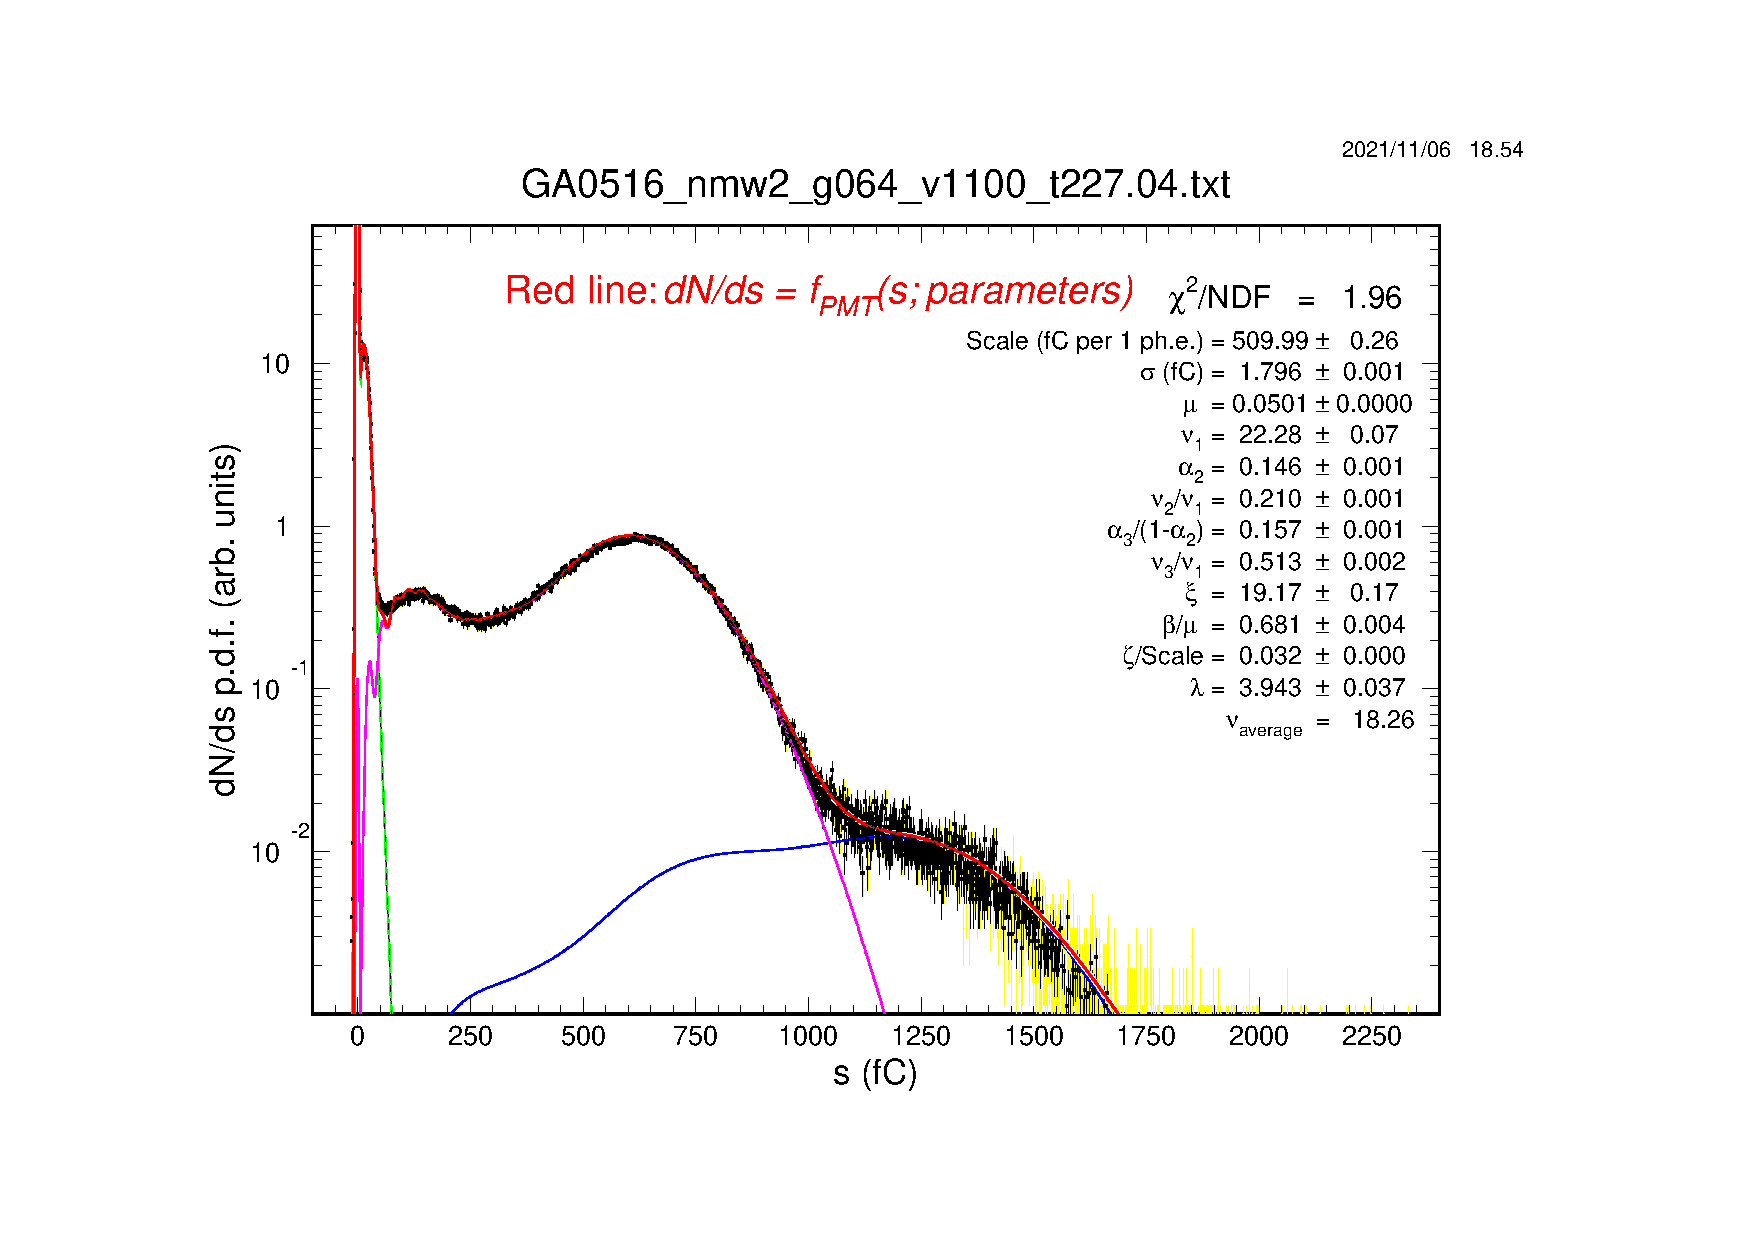
\includegraphics[clip=true,trim=100 75 140 100,width=.49\textwidth,height=.25\textwidth]
                    {figures/GA0516_3d.pdf}}
  \caption{Signal amplitude probability distributions for PMT GA0516 (H12700), pixel 4, wheel position 2, at HV = 1000 V ((a) and (c)) and at HV = 1100 V ((b) and (d)). (a) and (b) run with 6 mm mask covering the full PMT face except pixel 4. (c) and (d) run with full PMT face open with the contribution to the spectrum from the crosstalk events approximated and parametrized by the analysis algorithm. Contributions to the spectra are shown by colors: red is the single photoelectron, blue - two or more photoelectrons, green-black dashed line shows the measurement function including the pedestal Gaussian and the crosstalk contribution. 
    }
\label{fig:GA0516_3}
\end{figure*}
\begin{figure*}[h!bt] 
\centering 
  \subfloat[6 mm mask, at HV = 1000 V]{%
    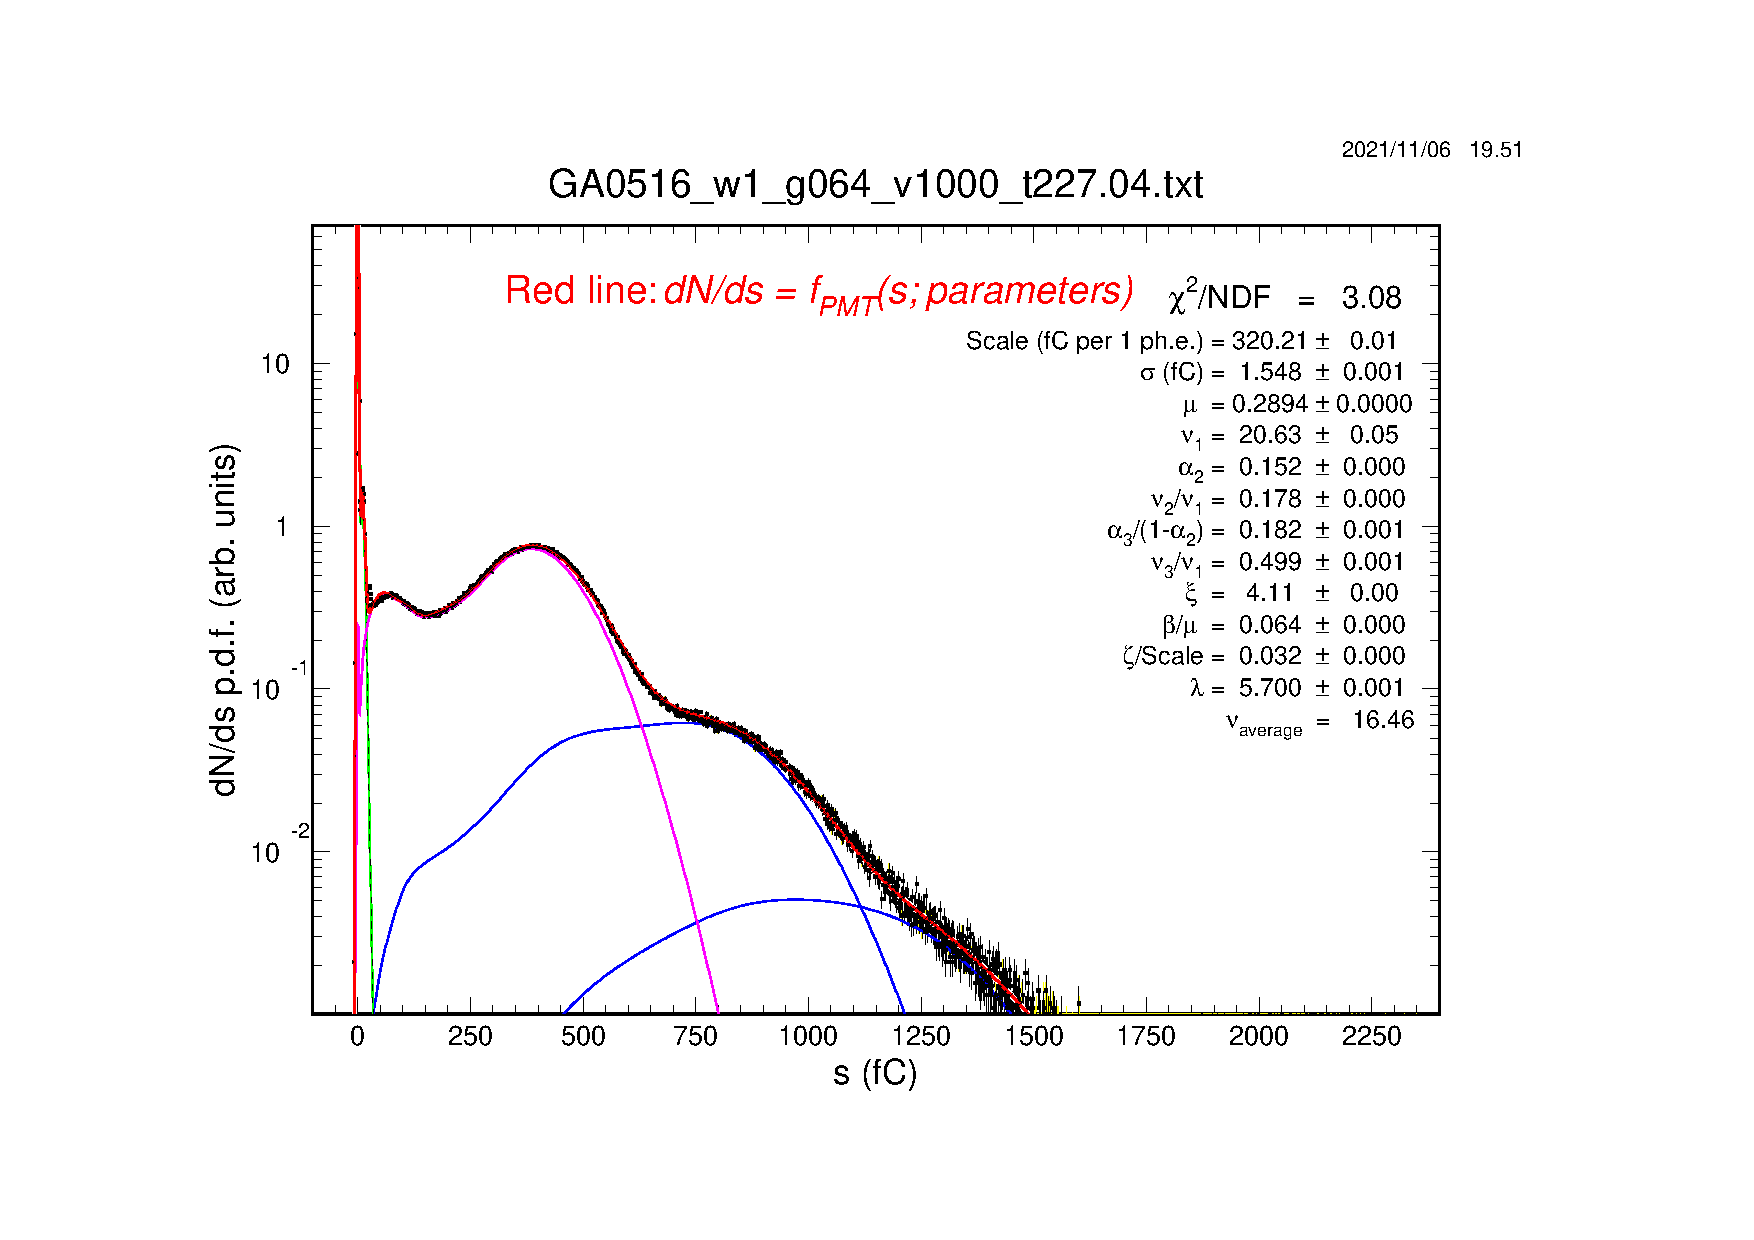
\includegraphics[clip=true,trim=100 75 140 100,width=.49\textwidth,height=.25\textwidth]
                    {figures/GA0516_4a.pdf}}
  \subfloat[6 mm mask, at HV = 1100 V]{%
    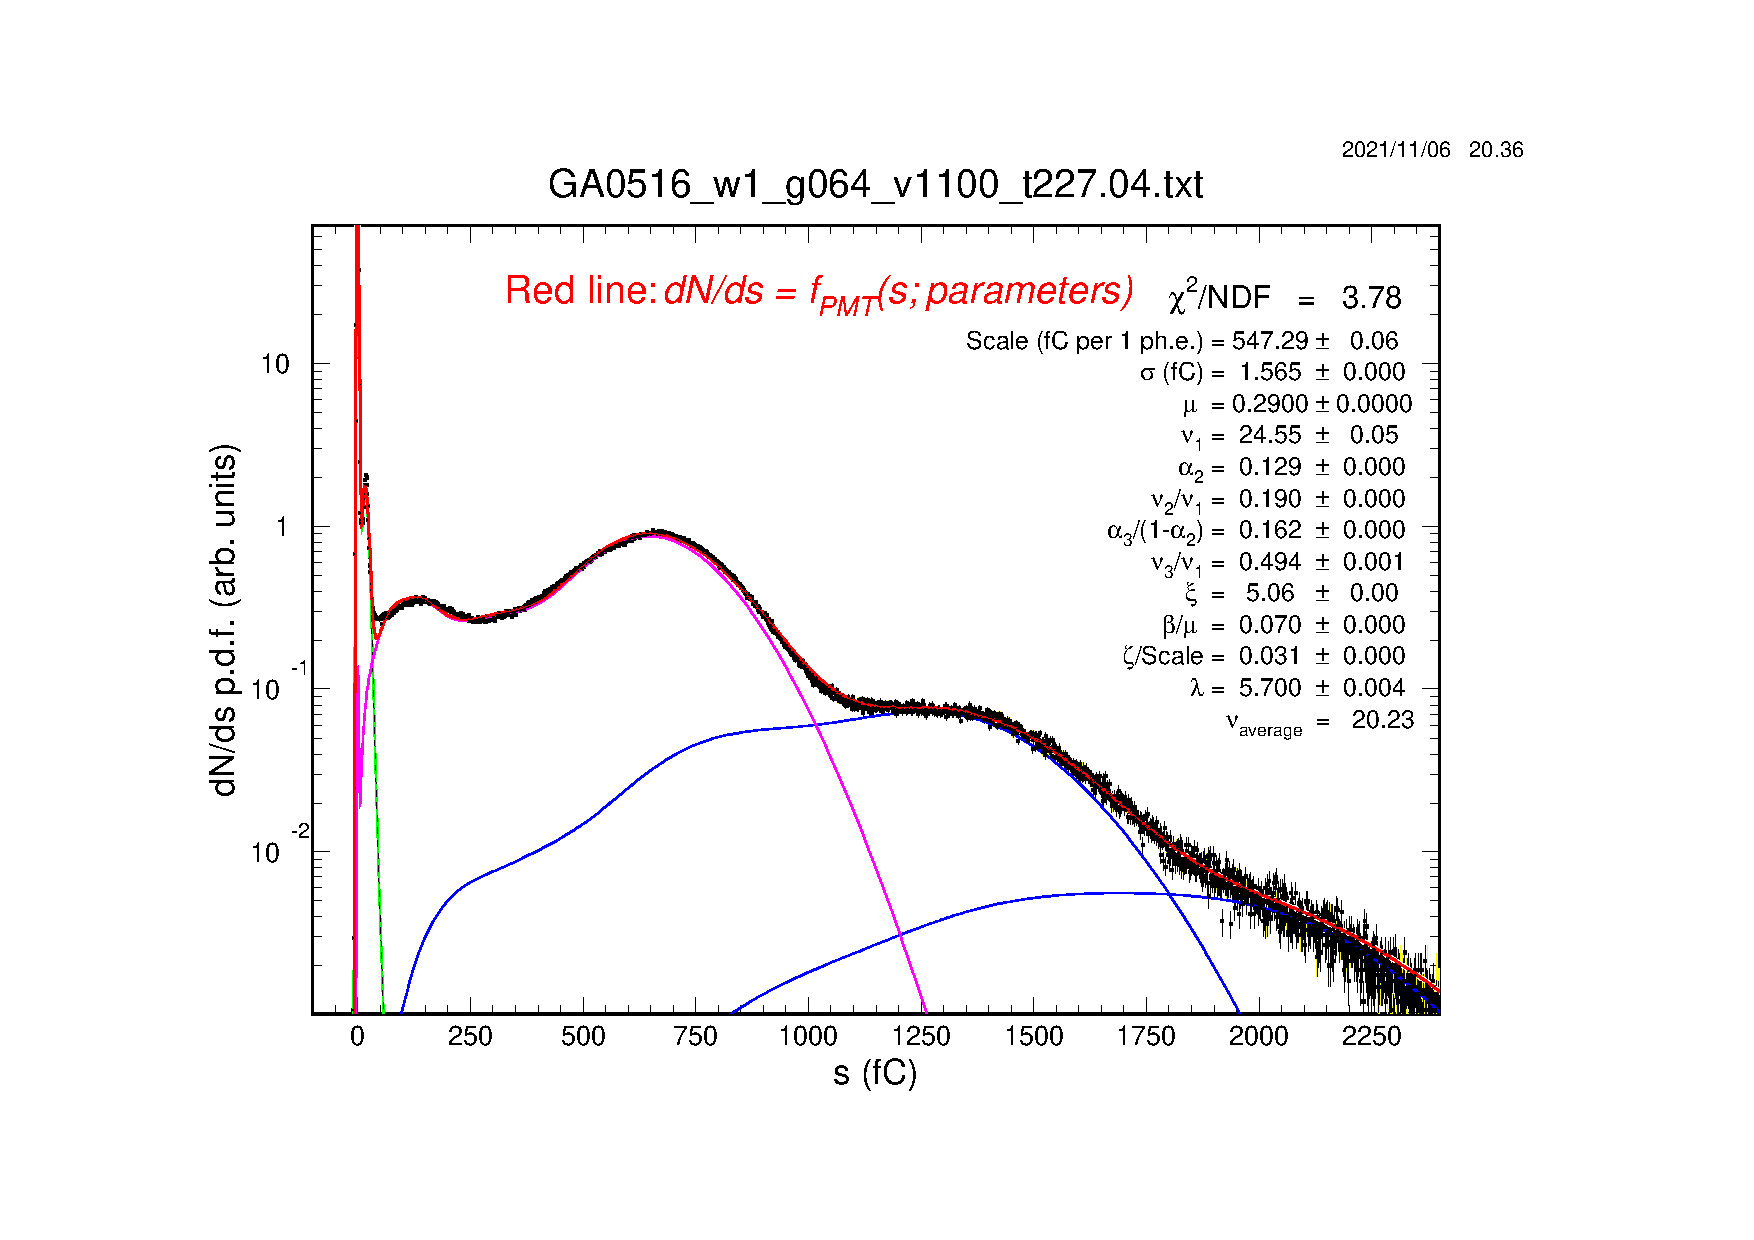
\includegraphics[clip=true,trim=100 75 140 100,width=.49\textwidth,height=.25\textwidth]
                    {figures/GA0516_4b.pdf}} \\
  \subfloat[No mask, at HV = 1000 V]{%
    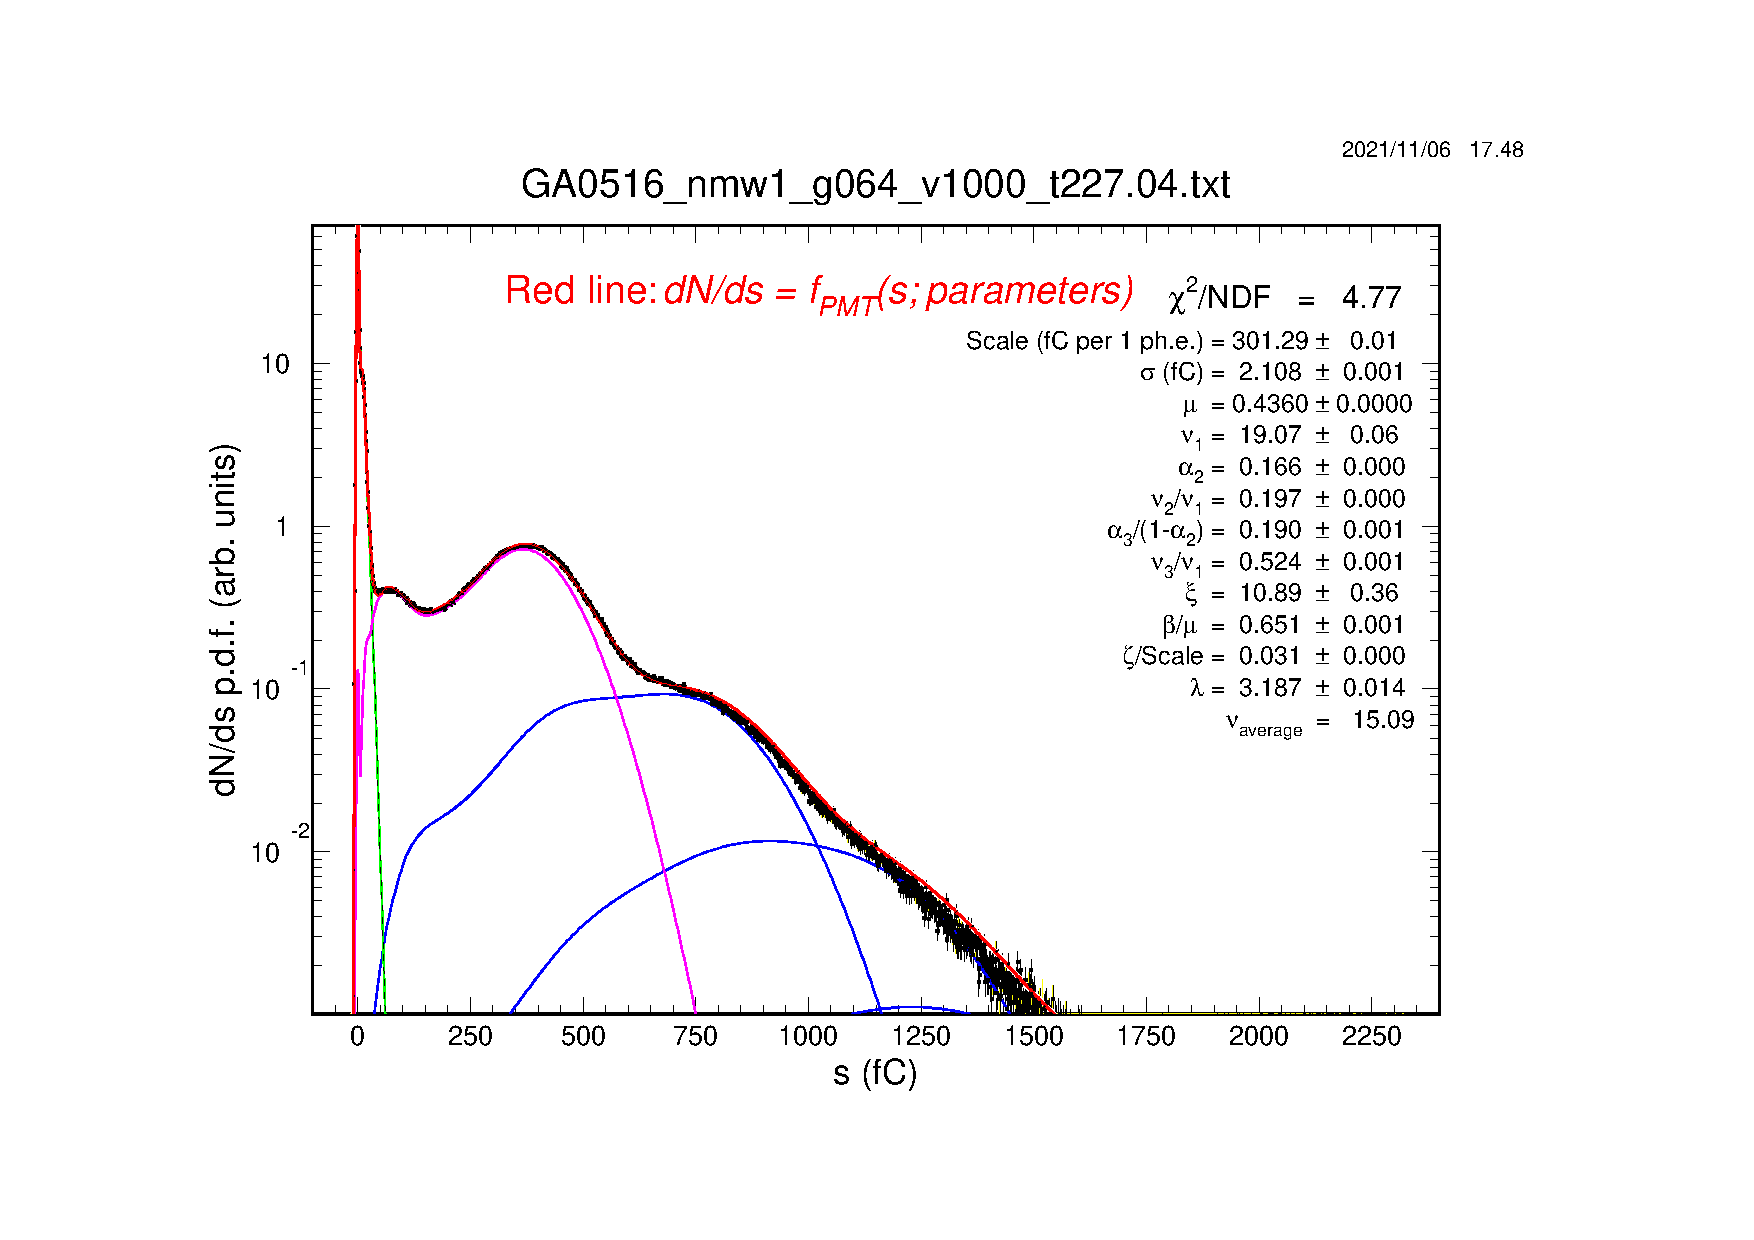
\includegraphics[clip=true,trim=100 75 140 100,width=.49\textwidth,height=.25\textwidth]
                    {figures/GA0516_4c.pdf}}
  \subfloat[No mask, at HV = 1100 V]{%
    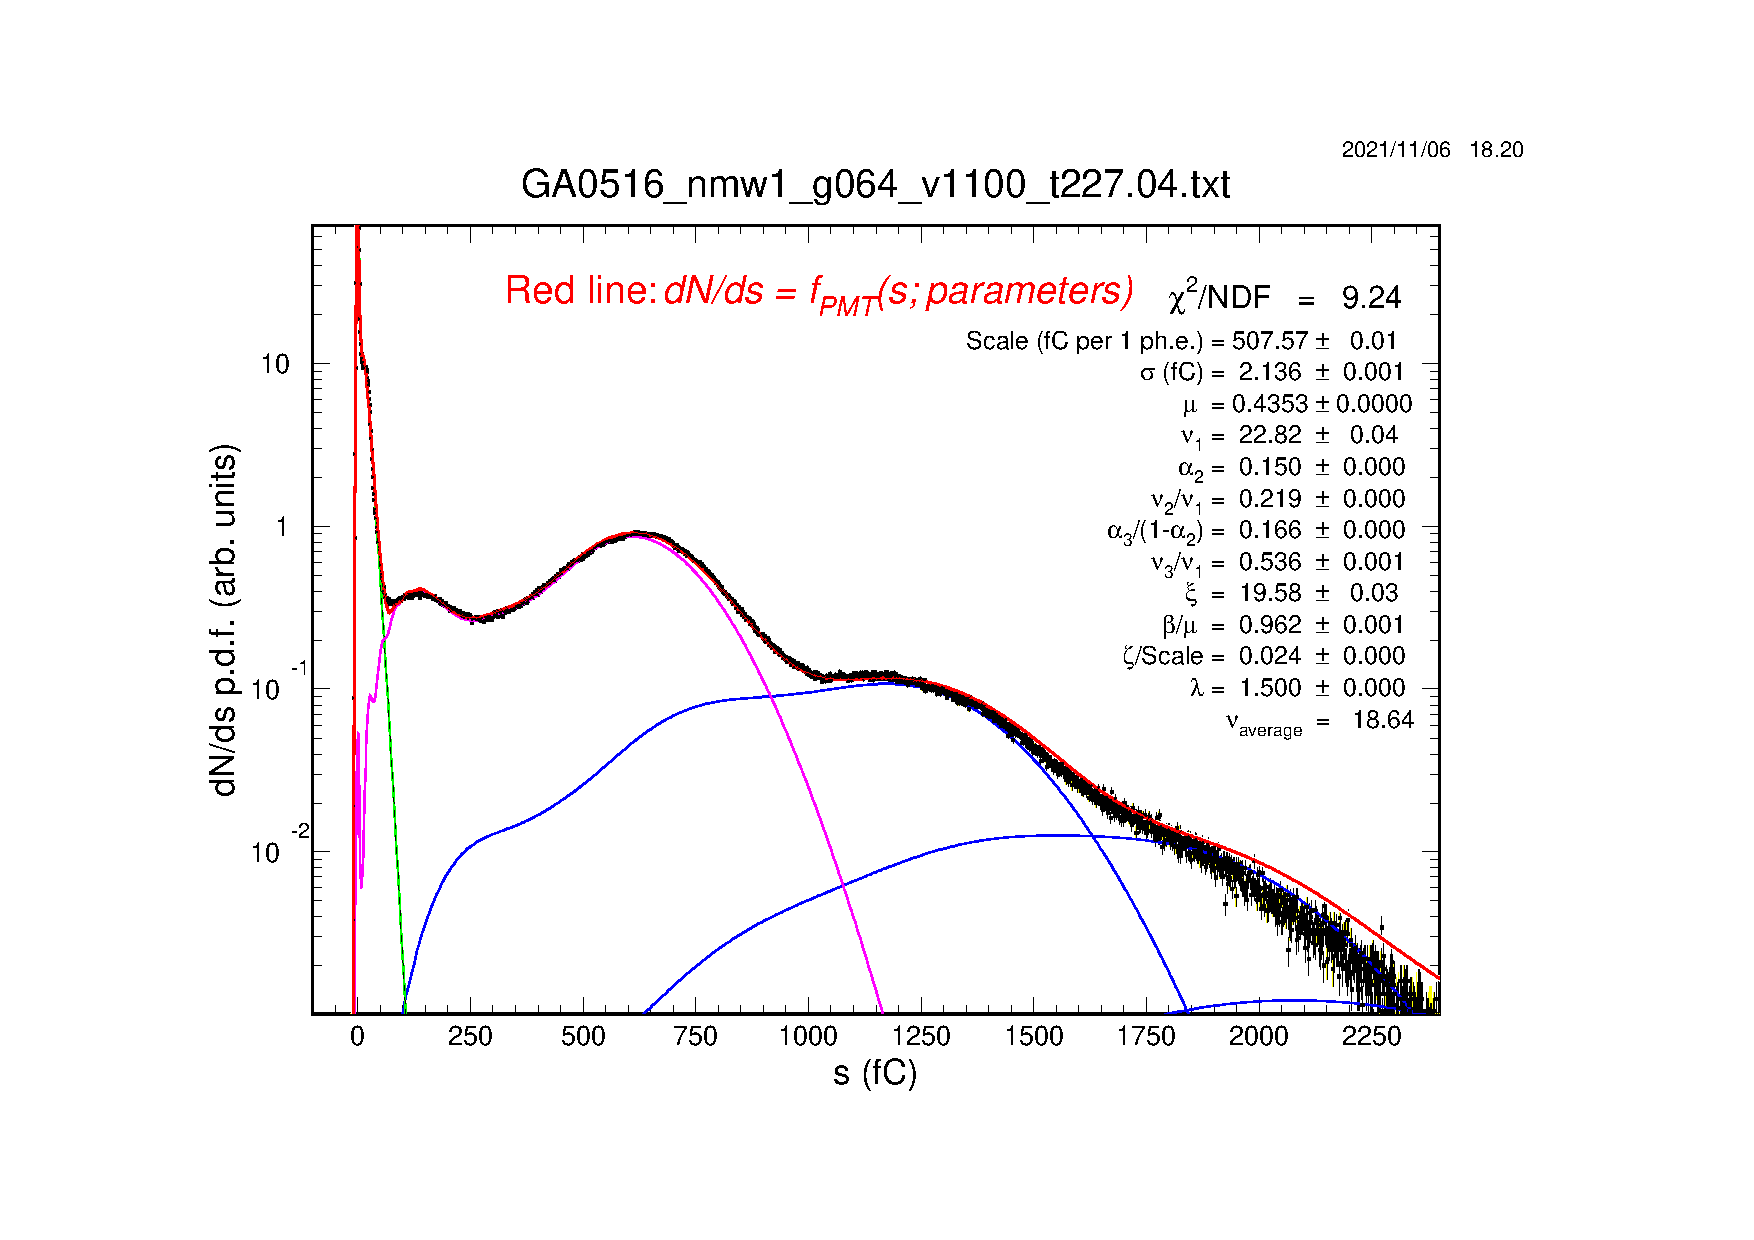
\includegraphics[clip=true,trim=100 75 140 100,width=.49\textwidth,height=.25\textwidth]
                    {figures/GA0516_4d.pdf}}
  \caption{Same as Fig.~\ref{fig:GA0516_3}, but at the wheel position 1. 
    }
\label{fig:GA0516_4}
\end{figure*}


\begin{figure*}[!ht]
	\centering
	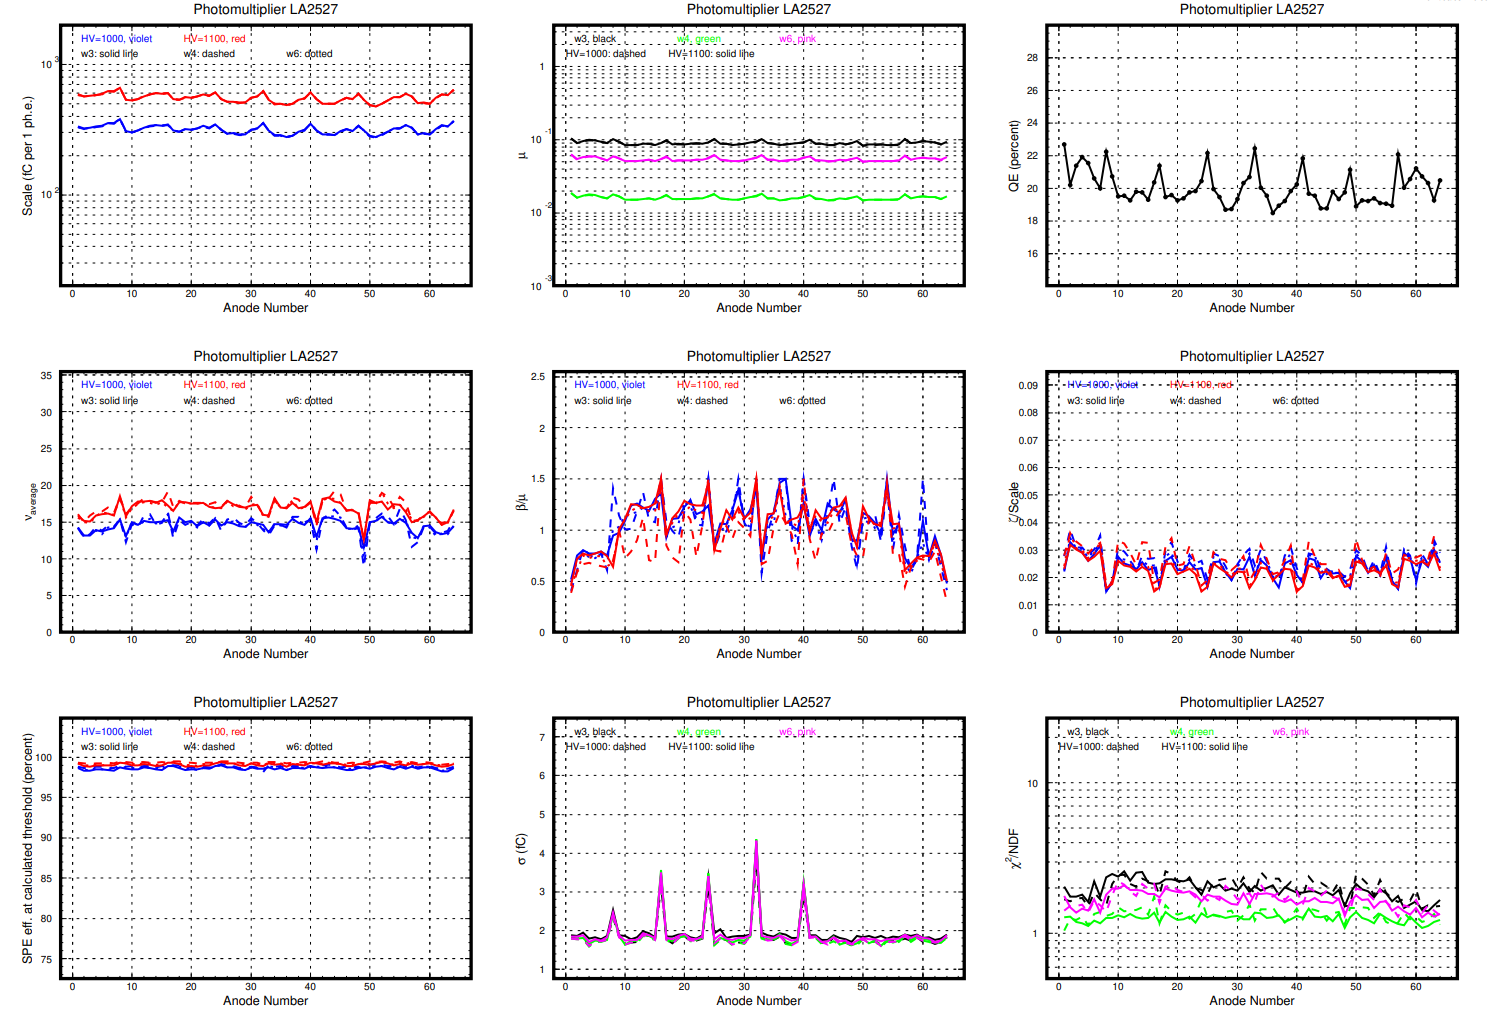
\includegraphics[width=1.0\textwidth,height=.7\textwidth]{figures/pavel_temp/LA2527_passport_temp.png}
	\caption{Illustration of the ``MAPMT passport'' plots for one of the PMTs, LA2527 (H12700). The standard six measurements included runs at three illumination settings (wheel positions 3, 4, and 6), each at two operating high voltage values (1000~V and 1100~V).}
	\label{fig:LA2527_passport}
\end{figure*}
\begin{figure*}[!ht]
	\centering
	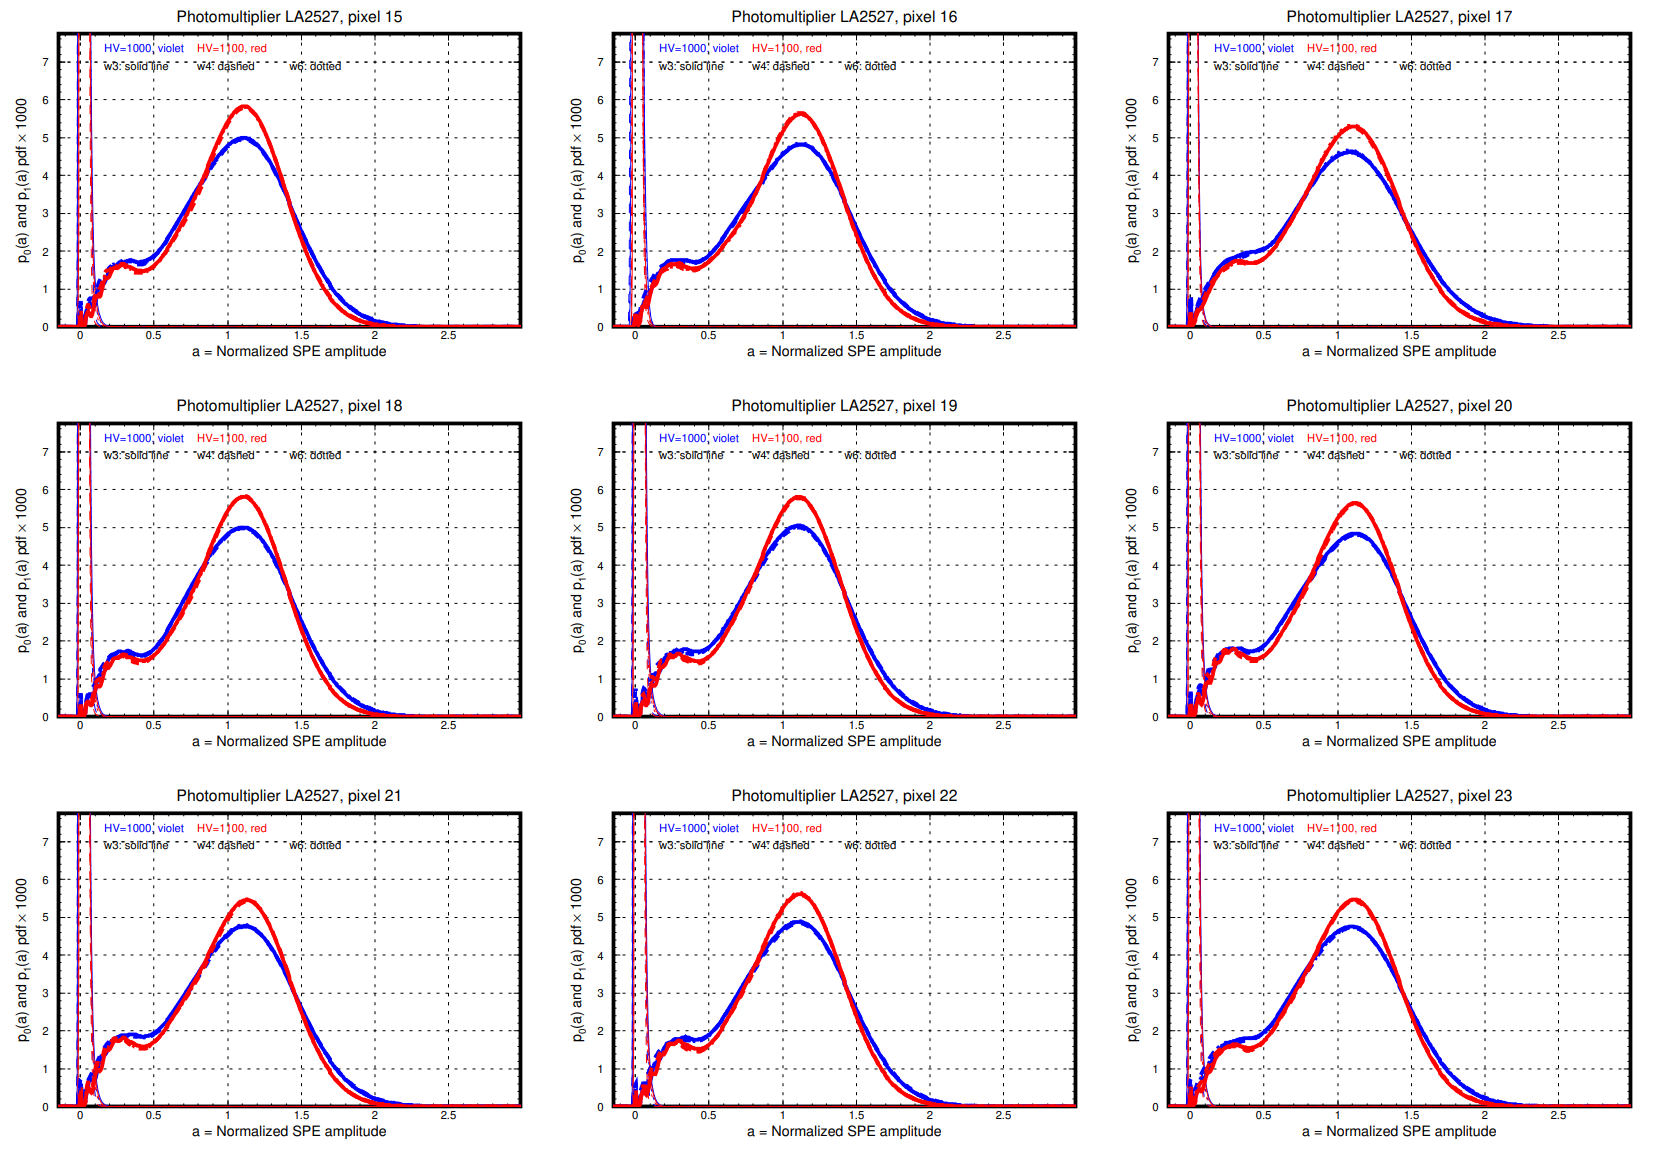
\includegraphics[width=1.0\textwidth,height=.7\textwidth]{figures/pavel_temp/LA2527_spectra_temp.png}
	\caption{Illustration of the ``MAPMT passport'' plots for one of the PMTs, LA2527 (H12700), continued. The standard six measurements included runs at three illumination settings (wheel positions 3, 4, and 6), each at two operating high voltages (1000~V, and 1100~V). Shown are the calculated SPE probability distribution functions $p_1(a)$, defined by the fit parameters resulting from the independent fitting procedures for each of the six settings. The blue color corresponds to the three sets at HV = 1000~V, and red - to the sets at HV = 1100~V. The parameters of the independent fits at three different illuminations result in very stable SPE shapes, essentially overlapping each other in the plots. The measurement functions $p_0(a)$ are shown as peaks around the pedestal at $a=0$ with the left sharp edge width corresponding to $\sigma$, and the right edge determined by the crosstalk.}
	\label{fig:LA2527_passport_spectra}
\end{figure*}

As a demonstration of the characterization procedure for the MAPMTs, Figs.~\ref{fig:CA7811}-\ref{fig:GA0516_4} show the measured signal amplitude probability distributions for one H8500 MAPMT pixel (CA7811, pixel 9) and one H12700 MAPMT pixel (GA0516, pixel 4) under various conditions, as well as their respective fit results. 
Figure ~\ref{fig:CA7811} and Fig.~\ref{fig:GA0516_1} illustrate the effect that the electronic crosstalk from neighboring pixels has on the measured SPE fit parameters. 
We collected two sets of data intended to reduce the contribution of crosstalk from neighboring pixels. 
In the first (as described in Section 5) we used a black sheet of paper to mask all pixels on a single MAPMT and punctured a 3~mm hole over the pixel of interest (see Fig.~\ref{fig:CA7811}a). 
However, with this setup, one cannot fully characterize the unmasked pixel, as there is some dependence of the measured signal on the location of the incident photon. 
To provide full coverage of a single pixel\textquotesingle s surface, another set of measurements was taken with a 6~mm x 6~mm square hole cut out over a single pixel. 
With this configuration, the full face of the pixel of interest was illuminated, while the neighboring pixels remained mostly covered by the black paper. 
However, there is still a non-negligible contribution from crosstalk with this configuration, due to imperfect alignment of the masks. 
This can be clearly seen in Fig.~\ref{fig:CA7811}b which shows the signal amplitude distribution with this 6~mm x 6~mm square hole cut out over pixel 9. 
One can see the contribution of the crosstalk appearing as a shoulder to the pedestal, albeit smaller than the crosstalk shoulder seen in Fig.~\ref{fig:CA7811}d where the full face of the MAPMT was illuminated. 

The resulting SPE fit parameters for Figs.~\ref{fig:CA7811}a-d indicate the inability of the model to fully describe the crosstalk in the H8500 MAPMTs. 
Most notably, in the data sets where the full-face of the MAPMT was illuminated (see Figs.~\ref{fig:CA7811}c-d) the $scale$ parameter changes by almost $7\%$ when the crosstalk is removed by the offline correlation analysis procedure compared to when it is kept in the data. 
Because the $scale$ parameter gives the average charge measured per photoelectron, it should be independent of the crosstalk. 
In contrast, we observe that the crosstalk in the H12700 MAPMTs can indeed be well described by the updated model, as is evident by comparing the fit parameters for Figs.~\ref{fig:GA0516_1}c-d. 
All parameters are consistent between the two fits, despite the fact that the crosstalk was removed by the offline analysis prior to performing the fit for Fig.~\ref{fig:GA0516_1}c. 
This result exemplifies the ability of the model to extract the SPE parameters from the measured signal amplitude distributions in a crosstalk-independent manner. 

The sample comparison between typical H8500 and H12700 MAPMTs as shown in Figs.~\ref{fig:CA7811} and \ref{fig:GA0516_1} generally confirms our decision to switch to H12700 as the MAPMT of choice for the RICH detector. In the previous study (Ref.~\cite{DEGTIARENKO20171}), using a different electronics front-end and data acquisition system, we observed that the values of the $\nu_{average}$ parameters were generally much smaller for H8500 than for the H12700, leading to a significant improvement of the expected efficiency of the H12700 MAPMTs to SPE events. In the previous study the amplitude resolution was not good enough to uncover the additional difference between the two models: the crosstalk spectra are significantly wider in the H8500, decreasing the expected SPE efficiency further, as compared to H12700. Wide crosstalk distributions in the H8500 overlap noticeably with the shapes of the model SPE functions and do not allow the model to isolate them, while for the H12700 MAPMTs the separation between the crosstalk and SPE distributions is reliable.  

The same sets of data were taken with the H12700 MAPMT high voltage set to 1100~V to compare with the results of Fig.~\ref{fig:GA0516_1} which were taken at 1000~V. 
The resulting amplitude probability distributions and fits are shown in Fig.~\ref{fig:GA0516_2}. 
As expected, both the $scale$ and $\nu_{average}$ parameters are larger when the high voltage is increased to 1100~V, while the parameters describing the crosstalk, $\beta/\mu$ and $\zeta/scale$, are fairly consistent. 
Furthermore, by comparing Fig.~\ref{fig:GA0516_2}c and Fig.~\ref{fig:GA0516_2}d, we observe the same desirable characteristic that the SPE fit parameters are consistent with or without the offline removal of the crosstalk events from the data even at a larger high voltage setting.


Finally, Fig.~\ref{fig:GA0516_3} and Fig.~\ref{fig:GA0516_4} show the signal amplitude probability distributions for the same pixel on MAPMT GA0516 at higher illumination intensities. 
Specifically, Fig.~\ref{fig:GA0516_3} shows the results when the filter wheel is at position 2, for high voltage settings 1000~V and 1100~V, both with the full MAPMT face illuminated, and with the 6~mm x 6~mm square hole mask cutout applied. 
Comparing Fig.~\ref{fig:GA0516_3}c to Fig.~\ref{fig:GA0516_1}d (full-face illumination, 1000~V), the $\mu$ parameter is almost a factor of 10 larger for the data collected with wheel position 2, but the characteristic parameters for the SPE response are consistent. 
The same can be said by comparing to the signal amplitude probability distribution in Fig.~\ref{fig:GA0516_4}c, which was measured at filter wheel position 1 (highest illumination). 
Even at roughly 100 times the light intensity, the resulting $scale$ parameter is consistent to that measured at low light intensity. 

Figure~\ref{fig:LA2527_passport} shows an example of the ``passport'' plots obtained for a single MAPMT - in this case, an H12700 PMT labeled LA2527. 
Each plot shows different parameters extracted from the fits to the signal amplitude probability distributions vs. the pixel number, resulting in 64 data points per curve.
In all plots (excluding the top-right plot), the fit results are compared for the data taken with wheel positions 1, 2, and 3, and high voltages 1000~V and 1100~V (6 different configurations in total).
As expected the $scale$ and $\nu_{average}$ parameters are independent of the light intensity, but change with the applied high voltage. 
This is due to the increased amplification at each dynode at higher applied voltages.
The $\beta/\mu$ and $\zeta/scale$ parameters that describe the crosstalk from neighboring photoelectrons remain somewhat consistent between the different experimental configurations. 
However, the $\beta/\mu$ passport plot shows the dependence of the frequency of crosstalk on pixel location. For example, the first 8 and last 8 pixels all have significantly lower $\beta/\mu$ parameters. These pixels are along the edge of the MAPMT and therefore have (at least) one fewer neighboring pixel than those in the center of the MAPMT.
Consequently, the $\beta$ parameter for the amplitude probability distributions in these pixels is lower. 

The measurement of the absolute photon flux on each pixel was discussed in Section 5. The QE is obtained for each pixel by combining this measurement with the average number of photoelectrons measured per laser pulse, $\mu$, which is extracted separately for each pixel as a parameter of the fit to the signal amplitude probability distribution. The resulting QE distribution is shown in the top-right plot of Fig.~\ref{fig:LA2527_passport}. These results indicate that on average the QE for each pixel of the H12700 MAPMTs is about 21$\%$ for incident photons with wavelength 470~nm.

The lower-right plot illustrates the quality of the SPE fit by showing the standard $\chi^2/NDF$ values for every fit, calculated for all bins in the measured spectrum with amplitudes above threshold. The accumulated number of events in each measured spectrum was very high and it is hard to expect an ideal model description with $\chi^2/NDF = 1$. The statistical quality of the fit was reasonably good for all measured spectra.

One final remark from the plots included in Fig.~\ref{fig:LA2527_passport} is that the SPE efficiency shown in the lower-left plot is slightly larger at 1100~V than at 1000~V. The efficiency was defined as the percent of SPE events above the threshold, which, in turn, was defined as the amplitude at which the number of events in the SPE distribution below the threshold was equal to the number of events in the crosstalk spectrum above it. The higher voltage leads to increased separation between the SPE spectra and the pedestal, corresponding to larger values of $\nu_{average}$, and thus increasing the efficiency. 

Figure~\ref{fig:LA2527_passport_spectra} shows the extracted SPE functions for 9 pixels on the same MAPMT, again for all 6 configurations. The probability distributions are given as a function of the normalized charge amplitude, $a$. The functions extracted from the data measured at 1100~V are noticeably more narrow around the peak than the data collected at 1000~V, in agreement with the previously noticed differences between the values of $\nu_{average}$ and the efficiency at the different high voltages. The plots also illustrate the pedestal measurement functions around $a=0$, including the crosstalk contributions. The pedestal functions and the SPE functions, measured independently at three illumination settings, visibly overlap, and thus illustrate the stability of the fitting procedure and validate the applicability of the model in its function to objectively extract the MAPMT characteristics.


\iffalse
The performance of MAPMTs was evaluated under certain high voltages.
The single photoelectron spectrum and the pixel efficiency for H12700 MAPMTs were tested and analyzed at 1000v, 1050v, 1075v, and 1100v.
The measurements performed at the reference supply voltage of 1000 V were compared to the measurements at different HV values in order to study the behavior of the MAPMT response as a function of the supply voltage.
As expected, it was found that the H12700 MAPMTs perform the best in the single photoelectron spectrum efficiency at higher voltages, especially at 1100v.
We see a significantly improved separation of the first photoelectron peak from the pedestal at higher voltage supplies (see~Fig.~\ref{fig:SPEhv}).
When the average deficiencies of the tested MAPMTs were analyzed, it was found that the average efficiency for 1000v, 1050v, 1075v and 1100v were approximately 4.6\%, 4.9\%, 5.0\%, and 5.2\%, respectively.
Therefore, the increase in detection efficiency is found to be over 10\% at 1100 V in comparison to 1000 V supply.
This separation is the crucial point for a single photon counting detectors such as CLAS12 RICH, where the occupancy is at the level of one photon per pixel.



It was also found that as the gain of the MAPMT increased, the efficiency ratio of 1100v to 1000v decreased.
The ratio is shown on~Fig.~\ref{fig:effratio} as a function of MAPMT gain reported by Hamamatsu.
The high voltage supply improves the performance of MAPMT dynode system, decreasing the fraction of the single photoelectron events below the pedestal peak.
This indicates that lower gain MAPMTs have a greater difference in the efficiencies at 1100v and 1000v, while higher gain MAPMTs have a smaller difference between the two voltage efficiencies.
The improvement for lower gain MAPMTs is more significant than for higher gain MAPMTs, because the high gain MAPMT has good separation of signal from pedestal even at the reference 1000 V.
Therefore, the low gain MAPMT benefit greatly from higher supply voltage.
The collected data are used to determine what high voltage the MAPMTs should be ran at to acquire the best results when the RICH detector is completed.


The parameters from Pavel's PMT response function are shown on the Fig.~\ref{fig:mu} and \ref{fig:characteristicPars} and correspond to the emission of the photoelectron ($\mu$), its collection and multiplication on the first dynode ($scale$ and $\nu$).
We have omitted other parameters that take into account the resolution effects of readout system or correspond to the cascade multiplication of the secondary electrons as they are out of scope focus of our analysis.
Given our requirements for single photoelectron signal sensitivity MAPMTs of our choice should be able to detect with high probability single photon that reaches photocathode.
In order to achieve this goal MAPMT should have high quantum efficiency of the photocathode as well as high collection efficiency of produced photoelectron combined with substantial signal multiplication to achieve good resolution of SPE peak.
These characteristics were studied in bulk for all 27520 channels (430x64) during the different light conditions and for different supplied HV values.


Fig.~\ref{fig:mu} shows the distribution of parameter $\mu$ which correspond to the average number of the photoelectrons produced during the measurements.
This parameters represents the convolution of the MAPMT photocathode quantum efficiency and laser setup light intensity.
Both characteristics should not depend on HV supply values and it is demonstrated on this figure by comparison of $\mu$ values extracted for the measurements at 1000 V and 1100 V.
However one can change the parameter by varying the laser light intensity which is evident from the left shift of $\mu$ values for lower light intensity measurements.

The other two free parameters are plotted on Fig.~\ref{fig:characteristicPars}.
They correspond to the average number of second-stage electrons produced on the first dynode by photoelectron (see~Fig.~\ref{fig:nu} and average signal amplitude for single photoelectron spectrum (see Fig.~{fig:scale}).
Both parameters characterize mainly the amplifying subsystem of MAPMT and therefore should depend on supplied HV.
The measurements at 1000 V and 1100 V confirm that amplification is improved at higher values of applied high voltage.
Traditionally the second parameter (gain) is often used to describe the amplification abilities of photomultipliers and often used in calibration and reconstruction procedures.
And it was shown that the extracted gains do not depend on the light conditions with a high degree of accuracy.
\fi
	  % Andrey
\section{Results}

This section reports on the study of 399 MAPMTs H12700, acquired for the RICH2 detector upgrade. All of them were tested in the same conditions by the groups of six mounted in the Maroc tiles and irradiated simultaneously. The test procedure included six different setup conditions: two sets of the high voltage applied (1000 V and 1100 V), and three laser light intensity settings at the wheel positions 3, 4, and 6. The data were accumulated and pre-processed to make the non-linearity corrections and to convert the amplitudes to the units of electric charge. After that the data were transferred to the ``parameterization factory'' computer workstation in which every accumulated spectrum was automatically analyzed and approximated with the 12-parameter fitting function, as it is explained in the earlier sections. Every PMT was issued the ``MAPMT passport'' document listing the fit parameters for every measurement, for all 64 anodes, showing the extracted SPE functions, and the parameter dependencies on pixel number, as illustrated in Figs. \ref{fig:LA2527_passport} and \ref{fig:LA2527_passport_spectra}. The most important parameters extracted from the analysis for every pixel are $scale$, measuring the average charge collected at the anode from the single photoelectron events; the average multiplicity $\mu$ of the photoelectrons per laser pulse, that can be converted to the quantum efficiency of the pixel when normalized to calibrated incoming light in the pulse; the calculated optimal threshold value for the separation of the single photoelectron events from pedestal (including the cross talk background), and corresponding estimate of the photodetection efficiency based on that value. Parameters of interest are also the characteristics of the photomultiplier, such as the evaluated in the model gain on the first dynode, amplitude width and intensity of the cross talk signal. The pedestal $\sigma$ parameter characterizes the quality of the Maroc measurement channel.

The six independent measurements in different conditions were used to verify the self-consistency of the results, using the model approximation features allowing the $scale$ parameter to be measured at various light conditions, ideally providing the same value, and similarly allowing the $\mu$ parameter (and hence the quantum efficiency) to be measured at various high voltages, also providing the same value. These features may be found in all ``MAPMT passports'', and also they are further illustrated in the following figures. Fig. \ref{fig:pglobal_sc} shows the distribution of $scale$ parameter through the whole data set, separately for different high voltage and illumination settings. The distributions are clearly identical if obtained in different illuminations, and the change in high voltage is seen as approximate multiplication of the $scale$ parameter by a factor about 2 when switching from HV = 1000 V to HV = 1100 V. Logarithmic scale in x axis in the plot helps to see the multiplication as a shift on the plot, roughly preserving the shape of the distribution. 

\begin{figure}[hbt]
	\centering
	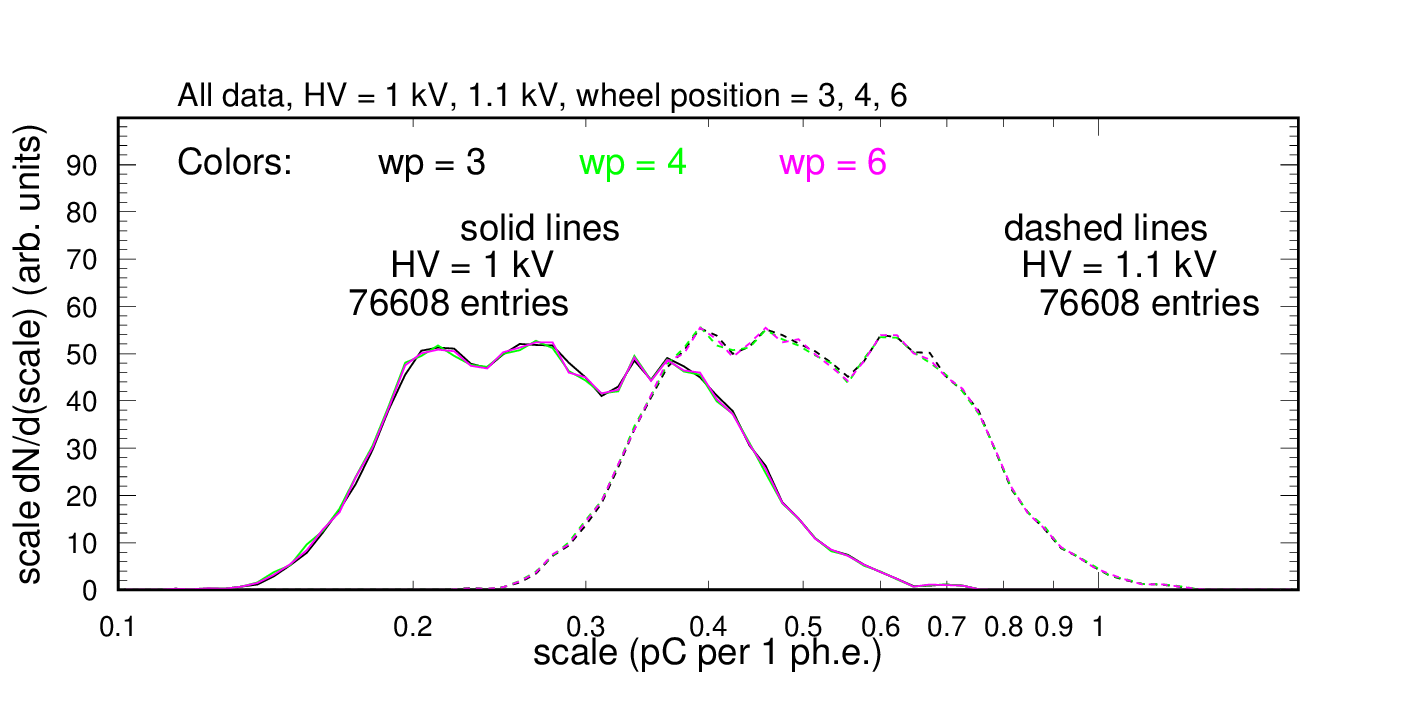
\includegraphics[width=0.98\linewidth,trim=0 15 50 35,clip]{figures/pglobal_sc.pdf}
	\caption{Distribution of $scale$ (average charge per ph.e) as determined by the fitting procedure for a set of 399 PMTs. All measured pixels contributed to the plots. Distributions measured at HV = 1000 V are shown by solid lines, the ones at HV = 1100 V by dashed lines. The three colors correspond to the three different illuminations (essentially on top of each other).
	}
	\label{fig:pglobal_sc}
\end{figure}

Fig. \ref{fig:pglobal_qe_all} shows the similar pattern for the $\mu$ parameter, with the difference that $\mu$ essentially does not depend on high voltage, but proportional to the light intensity. The plot shows that the distributions at different high voltages are on top of each other at a given light intensity, but shift in log scale when light intensity changes. In the plot the parameter $\mu$ is shown normalized to the number of photons coming to each pixel in the ``wheel position 3'' setting, to provide the value of quantum efficiency in it. 
\begin{figure}[hbt]
	\centering
	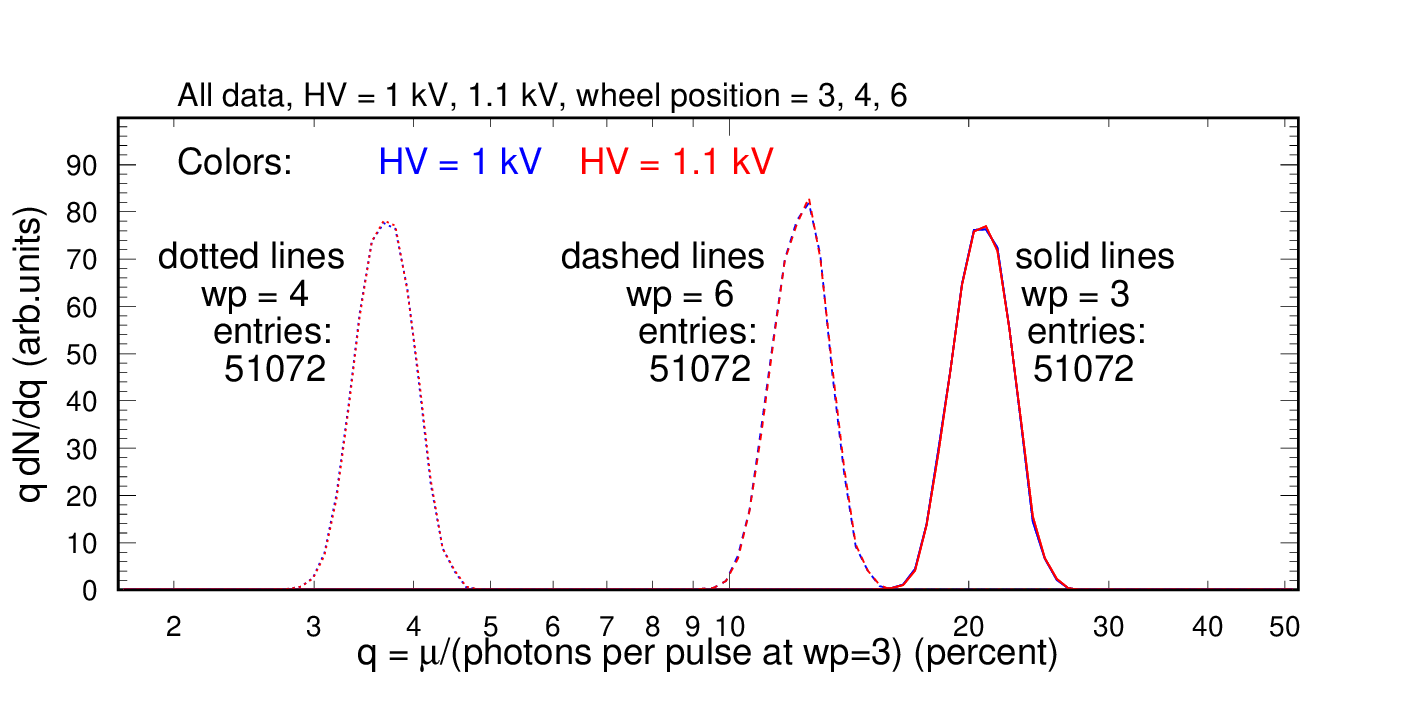
\includegraphics[width=0.98\linewidth,trim=0 15 50 35,clip]{figures/pglobal_qe_all.pdf}
	\caption{Distribution of $\mu$ divided by the measured number of photons per pulse at wheel position 3. All measured pixels contributed to the plots. Distributions measured at HV = 1000 V are shown by violet, the ones at HV = 1100 V by red color (essentially on top of each other). The three line styles (dotted, dashed, and solid) correspond to different illumination. For the data collected at wheel position 3, this ratio is the quantum efficiency of the individual pixels.}
	\label{fig:pglobal_qe_all}
\end{figure}
\begin{figure}[h!bt]
	\centering
	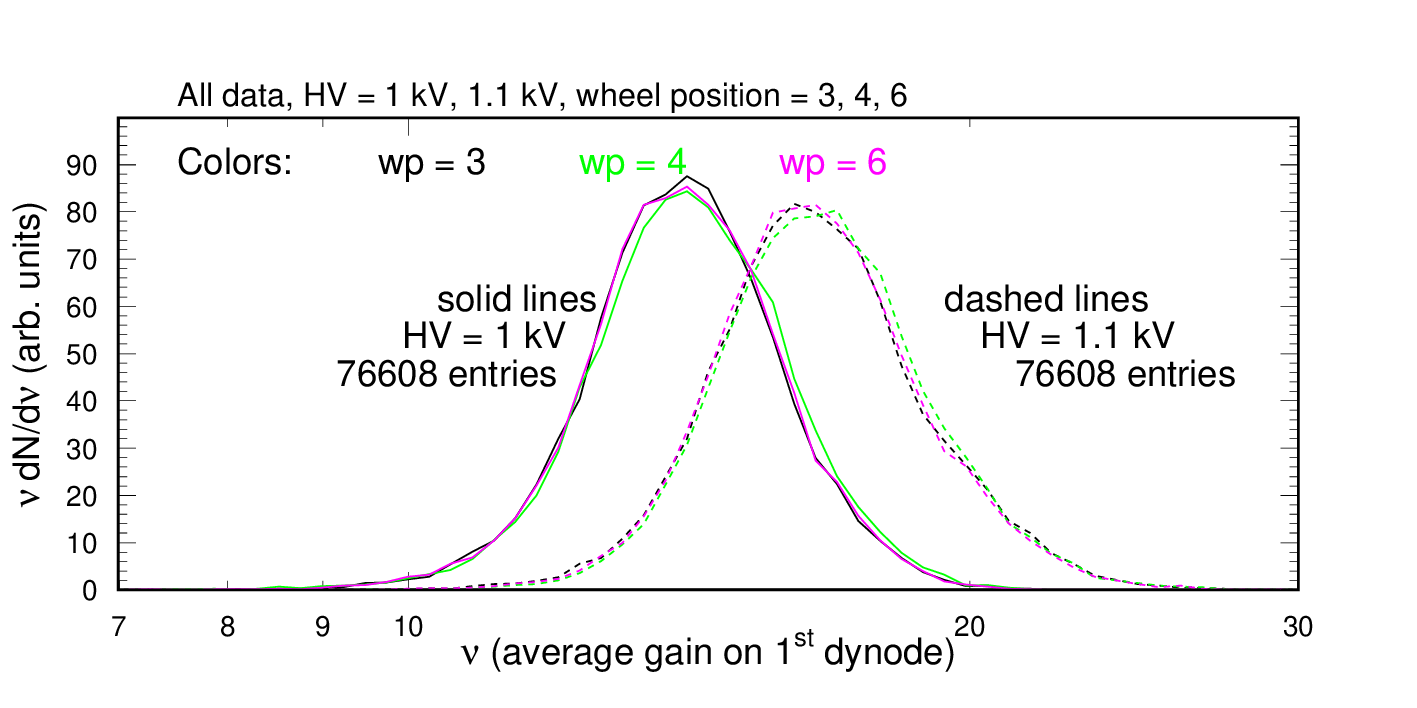
\includegraphics[width=0.98\linewidth, trim=0 15 50 35,clip]{figures/pglobal_nu.pdf}
	\caption{Distribution of $\nu$ (average gain on 1st dynode) as determined by the fitting procedure for a set of 399 PMTs.}
	\label{fig:pglobal_nu}
\end{figure}



\begin{figure}[h!bt]
	\centering
	\includegraphics[width=0.98\linewidth, trim=0 15 50 35, clip]{figures/pglobal_sc.pdf}
	\includegraphics[width=0.98\linewidth, trim=0 15 50 35, clip]{figures/pglobal_nu.pdf}
	\caption{Distribution of scale (average charge per ph.e) and $\nu$ (average gain on 1st dynode) as determined by the fitting procedure for a set of 399 PMTs.}
	\label{fig:pglobal_sc_nu}
\end{figure}

\begin{figure}[h!bt]
	\centering
	\includegraphics[width=0.98\linewidth, trim=0 15 50 35, clip]{figures/pglobal_Rs.pdf}
	\includegraphics[width=0.98\linewidth, trim=0 15 50 35, clip]{figures/pglobal_Rn.pdf}
	\caption{Scale and $\nu$ averaged over three different illumination settings (wheel positions 3, 4, and 6).}
	\label{fig:pglobal_Rs_Rn}
\end{figure}

\begin{figure}[h!bt]
	\centering
	\includegraphics[width=0.98\linewidth, trim=0 15 50 35, clip]{figures/pglobal_mHV.pdf}
	\caption{The ratio of the $\mu$ parameters from the fit results at HV = 1100 V to the results at HV = 1000 V.}
	\label{fig:pglobal_mHV}
\end{figure}


\begin{figure}[h!bt]
	\centering
	\includegraphics[width=0.98\linewidth, trim=0 15 50 35, clip]{figures/pglobal_qe_all.pdf}
	\caption{Distribution of $\mu$ divided by the measured number of photons per pulse at wheel position 3. For the data collected at wheel position 3, this ratio is the quantum efficiency of the individual pixels.}
	\label{fig:pglobal_qe_all}
\end{figure}

\begin{figure}[h!bt]
	\centering
	\includegraphics[width=0.98\linewidth, trim=0 15 50 35, clip]{figures/pglobal_eff.pdf}
	\caption{Distribution of the measured efficiency for all pixels at wheel position 4.}
	\label{fig:pglobal_eff}
\end{figure}

\begin{figure}[h!bt]
	\centering
	\includegraphics[width=0.98\linewidth, trim=0 10 15 10, clip]{figures/R_scale_maroc_avg.png}
	\caption{Evaluated precision of the scale parameter measurement for the two high voltage settings.}
	\label{fig:R_scale_maroc_avg}
\end{figure}


\begin{figure*}[hbt]
	\centering
	\begin{subfigure}[c]{0.4\linewidth}
		\centering
		\includegraphics[width=\linewidth, trim={0mm 0mm 0mm 19mm},clip]{figures/pglobal_sc2d.pdf}
		\caption{Average scale, HV = 1.0 kV (pC per 1 ph.e)}
		\vspace{0mm}
	\end{subfigure}%%
	\begin{subfigure}[c]{0.4\linewidth}
		\centering
		\includegraphics[width=\linewidth, trim={0mm 0mm 0mm 19mm},clip]{figures/pglobal_qe.pdf}
		\caption{Average Quantum Efficiency (percent)}
		\vspace{0mm}
	\end{subfigure}%%
	\vspace{3mm}
	\begin{subfigure}[c]{0.4\linewidth}
		\centering
		\includegraphics[width=\linewidth, trim={0mm 0mm 0mm 19mm},clip]{figures/pglobal_beta.pdf}
		\caption{Average cross-talk relative to $\mu$}
		\vspace{0mm}
	\end{subfigure}%%
	\begin{subfigure}[c]{0.4\linewidth}
		\centering
		\includegraphics[width=\linewidth, trim={0mm 0mm 0mm 19mm},clip]{figures/pglobal_zeta.pdf}
		\caption{Average cross-talk width relative to scale (percent)}
		\vspace{0mm}
	\end{subfigure}%%
	\vspace{3mm}
	\begin{subfigure}[c]{0.4\linewidth}
		\centering
		\includegraphics[width=\linewidth, trim={0mm 0mm 0mm 19mm},clip]{figures/pglobal_eff2d.pdf}
		\caption{Average efficiency, wp = 3, HV = 1.0 kV (percent)}
		\vspace{0mm}
	\end{subfigure}%%
	\caption{Two dimensional plots showing the average (a) scale, (b) quantum efficiency, (c) cross-talk relative to $\mu$, (d) cross-talk relative to scale, and (e) efficiency as a function of pixel location.}
	\label{fig:2d_avg_fit_results}
\end{figure*}



Large number of MAPMTs from Hamamatsu (XX of H8500 type, and XXX of H12700 type) were studied using the dedicated test stand at JLab. Their performance as single photon detectors was evaluated and characterized in conditions close to their future operations in the CLAS12 RICH detector.


Parameters of the single photoelectron response function of every pixel were extracted using the SPE spectra approximations in our mathematical model, modified to take into account the effects of the signal cross-talk between the neighboring pixels. The stability and consistency of the parameter values measured in different conditions of illumination and at different applied high voltages allows to characterize the intrinsic features of every pixel, independent on the measurement conditions. Absolute quantum efficiency and electronic gain of every channel, as well as the set of parameters describing variable shapes of the SPE functions were measured.


The parameter database accumulated as the result of this work may be used for the selection of the PSPMTs for installation in the RICH detector, and for the optimization of the future run parameters, such as the tube placement selection, setting the values of operating high voltage, electronics gains and thresholds in the detector.


The data also provide the opportunity to evaluate the spread of such parameters in the mass production of the PSPMT devices as the channel gains, quantum efficiencies, SPE spectral shapes, parameters of the cross-talk, - across the face of each tube, and across the whole set. The results show that the quality of PSPMT mass production at Hamamatsu is high and satisfies our needs in the good quality single photoelectron detection.



%We saw that although there is little difference in crosstalk signals, the H12700 PMTs suffer less from dark current, have narrower SPE spectra, and have higher $\mu$ and relative efficiency values.
%An example plot of the $\mu$'s and relative efficiencies of H8500 and H12700 PMTs with similar low and high gains is shown in Figure \ref{efficiency}.

%We see that the relative efficiency is closely related to the $\mu$ which is on average, over all pixels at all voltages for all the PMTs we tested, $29\pm5$ percent higher in H12700 than H8500 MAPMTs. One concern with these $\mu$ measurements however is that the laser system used to measure these PMTs was only incident on a portion of each pixel, consequently missing their sum total effect and pinpointing possible spatial dependencies which should be further studied and perhaps remeasured with a fully illuminated MAPMT instead of collimated pinpoint laser light. In terms of crosstalk for the two varieties of MAPMT the H12700s appear to be better than the H8500s. The H12700s have a decrease in crosstalk by nearly a factor of two. Additional studies of dark current in the H12700s would be useful, as the dark current is usually dominated by individual pixels or bad regions of the PMT instead of spread around evenly like in the H8500s, but overall the two varieties are not very different in terms of dark current.			  % All
\section{Conclusion}

As a part of CLAS12 RICH detector upgrade at Jefferson Lab, we have conducted a mass study of 399 H12700 MaPMTs from Hamamatsu, with the goal to evaluate every tube and characterize every pixel in terms of their gain, quantum efficiency, crosstalk contribution, and optimized threshold for detecting single Cherenkov photons. The dedicated test setup included a precision picosecond laser, 
gears for the  positioning of the laser beam in the setup,
RICH detector front-end electronics, and fully automated data acquisition and control systems. The non-linearity of the data acquisition, the ADC-to-charge conversion calibration parameters of every channel, and the absolute calibration of the number of laser photons reaching every pixel in every event were measured in special separate experiments. The bulk measurements consisted of six expositions of every group of six MaPMTs at three levels of low light and two applied high voltages, 1000~V, and 1100~V. The systematic uncertainties dependent on the MaPMT placement in the group of six were evaluated and found to be within the final parameter uncertainties.

In a set of dedicated detailed studies we observed and quantified the pixel-to-pixel signal crosstalk using a two-dimensional amplitude distribution analysis. Using several representative MaPMTs of both types we found that the H8500 model is characterized by quite significant amplitude spectral contributions to a given pixel from its neighbors in the matrix, with such crosstalk contributions reaching up to 50\% of the spectral amplitude. At the same time, the crosstalk in H12700 MaPMTs was generally less than about 3-5\%. Methods of separating and taking into account the crosstalk contributions to the amplitude distributions from any pixel were developed, using the two-dimensional analysis, and also approximating and evaluating the contributions based on the spectral shape using the computational model. The first approach is applicable to all MaPMTs studied, but it is labor intensive and works correctly only in the conditions of extremely low light in the tests. The second approach works well for the H12700 MaPMTs and was used for the bulk measurements.

The accumulated amplitude spectra were corrected to the non-linearity of the data acquisition and converted to the calibrated total charge distributions. The recently published state-of-the-art computational model, describing photon detector response functions measured in conditions of low light, was extended to include the successful description of the crosstalk contributions to the spectra from the neighboring pixels. The updated model was used to parameterize and extract the SPE response functions of every pixel, and characterize its properties such as gain, quantum efficiency, and crosstalk, and to determine the optimal signal threshold values to evaluate its efficiency to Cherenkov photons. The stability and reproducibility of the extracted parameter values were verified by the comparison of the six independent measurements of each pixel, allowing us to evaluate the uncertainties in the measurements of the major model parameters. One of the extracted parameters, the average multiplication of a photoelectron on the first dynode $\nu$ was found significantly larger on the H12700 compared to the H8500 MaPMTs. That difference corresponds to the resulting difference between the SPE efficiency of the two models.  That observation, together with much smaller crosstalk contributions, generally confirms our early decision to switch to the H12700 as the MaPMT of choice for the RICH detector.

The database of extracted parameters will be used for the final selection and arrangement of the MaPMTs in the new RICH detector, and for determining their optimal operation parameters, such as operating high voltage, gain, and threshold of the front-end electronics. A good model description of the measured amplitude distributions from MaPMT pixels, including the crosstalks, will allow using the parameterization in the Monte Carlo simulations of the detector. The results show that the quality of the H12700 MaPMT mass production at Hamamatsu is high, satisfying our needs in the good position-sensitive single photoelectron detectors.



\section{Acknowledgements}
This material is based upon work supported by the U.S. Department of Energy, Office of Science, Office of Nuclear Physics under contract DE-AC05-06OR23177, and in part by DOE Grant No. DE-FG02-04ER41309, DOE Grant No. DE-FG02-03ER41231 and NSF Award no: 2012413. 
We sincerely thank 
Bishnu Karki,
Charles Hanretty,
Aiden Boyer,
Chris  Cuevas,
Matteo Turisini, and
Carl Zorn
for their technical support and help in taking and analyzing the experimental data. We would
also like to thank 
Patrizia Rossi, 
Marco Contalbrigo, 
Marco Mirazita,
Kyungseon Joo,
and Zhiwen Zhao
for the fruitful discussions, continuous support, and interest in this work. Special thanks to Danial Carman for proofreading the article and making valuable comments.		  % All
%%%%%%%%%%%%%%%%%%%%%%%%%%%%%%%%%%%%%%%%%%%%%%%%%%%%%%%%%%%%%%%%%%%%%%%%%%

\bibliographystyle{elsarticle-num-names}
\bibliography{RICH}

\newpage
\newpage
\appendix
\section{}
\label{AppendixA}

In the case of the H12700 MAPMTs, the signal amplitudes of the crosstalk contributions from different neighboring pixels were found to be relatively small and similar to each other, allowing us to use in the model a single average spectral term for all neighbors of a given pixel. Each crosstalk contribution comes from a single electron in one of the neighboring pixels, their average number in one measurement $\beta$ is expected to be comparable with $\mu$, and multiple crosstalk events in one measurement happen independently. That means that the probability of observing $i$ crosstalk contributions in one event is distributed according to a Poisson distribution
\begin{equation}
\label{CTPoisson}
 P(i;\beta) = \frac{\beta^{i} e^{-\beta}}{i!}.
\end{equation}
Poisson-like shapes of the general spe distribution functions suggest a shape of the crosstalk contribution in the form of a Poisson distribution, scaled to represent the portion of the charge generated in the neighboring pixel, transferred to the pixel studied. The representation of such a distribution for one crosstalk electron takes the form
\begin{equation}
\label{C1Poisson}
 C_1(j) = P(j;\lambda) = \frac{\lambda^{j} e^{-\lambda}}{j!},
\end{equation}
where $j$ is a non-negative integer, corresponding to the amplitude values $a_j = j \zeta / \lambda $, relating the discrete Poisson scale to the set of $a$ values, such that the average crosstalk contribution to the measurement function from one crosstalk electron was equal to the value of the $\zeta$ parameter (the average $\langle j \rangle$ in Eq.~(\ref{C1Poisson}) equals to $\lambda$).

The corresponding distributions for the events with $i$ crosstalk electrons then take the form of convolution powers, which can be explicitly calculated in the case of Poisson distributions: 
\begin{equation}
\label{CiPoisson}
 C_i(j) = C_1^{*i}(j) = P(j;i\lambda).
\end{equation}

Thus, similar to Eq.~(13) in Ref.~\cite{DEGTIARENKO20171}, the discrete distribution can be represented as a function of the normalized amplitude $a$ in the form of the infinite sum of correspondingly weighted delta-functions, one per each value of $j \geq 0$:
\begin{equation}
\label{deltaf}
  D_{ct}(a)= \sum\limits_{j=0}^{\infty}
  \delta \left (a - \frac{j\zeta}{\lambda} \right )
   \sum\limits_{i=0}^{\infty} P(i;\beta) C_i(j) .
\end{equation}
The convolution of this distribution with the Gaussian measurement function (sigma equal to $\sigma_a$) will result in a continuous function similar to Eq.~(15) in Ref.~\cite{DEGTIARENKO20171}:
\begin{equation}
\label{RCmodel}
  R_{ct}(a)= \sum\limits_{j=0}^{\infty} \frac{1}{\sqrt{2 \pi} \ \sigma_a} 
  \exp{\left [- \frac{(a - j \zeta / \lambda)^{2}}{2 
\ \sigma_a^{2}} \right ]}
   \sum\limits_{i=0}^{\infty} P(i;\beta) C_i(j) .
\end{equation}

The new function $R_{ct}(a)$, parametrically dependent on $\sigma_a$, $\beta$, $\zeta$, $\lambda$, describes the effective measurement function applied to every signal. The recorded signals are the results of the convolution with this function. In particular, in the events with no photoelectrons ($m=0$), the pedestal distribution takes the form of $R_{ct}(a)$. For a given set of parameters the function $R_{ct}(a)$ is evaluated numerically in the model implementation and then used in the calculations as described in Ref.~\cite{DEGTIARENKO20171}, by replacing the measurement function $R(a)$ with $R_{ct}(a)$ in convolution with the $D(a)$ function in Eq.~(14) in Ref.~\cite{DEGTIARENKO20171}. The function $D(a)$ as defined in Eq.~(13), Ref.~\cite{DEGTIARENKO20171}, much like the function $D_{ct}(a)$ in Eq.~(\ref{deltaf}) in this work, represents an infinite set of delta-functions, and the convolution calculation just needs the values of the tabulated function $R_{ct}(a)$ in all the final sums. The new equivalent for Eq.~(16) in Ref.~\cite{DEGTIARENKO20171} is thus
\begin{equation}
\label{GCmodel}
  G_{ct}(a,n;\sigma_a,\beta,\zeta,\lambda)= R_{ct}(a-n/\nu;\sigma_a,\beta,\zeta,\lambda).
\end{equation}
The new function $G_{ct}(a,n;\sigma_{\mathrm{eff}},\beta,\zeta,\lambda)$ is then used to replace the function $G(a,n;\sigma_{\mathrm{eff}})$ in the final model equation, Eq.~(36) in Ref.~\cite{DEGTIARENKO20171}, keeping the same form. The change is that instead of being a standard Gaussian, the measurement function is now distorted by the crosstalk contribution, requiring three extra parameters to approximate the data.
		  % All

\end{document}
